% chap_03b.tex: fragment included inside Chapter 3 with % chap_03b.tex: fragment included inside Chapter 3 with % chap_03b.tex: fragment included inside Chapter 3 with % chap_03b.tex: fragment included inside Chapter 3 with \input{chap_03b}.
% It holds three sections: security and access management, the technical
% challenges with the solutions we adopted, and the evaluations and tests.

\section{Phone Booking}\label{sec:booking}

Phone booking is the main feature of Riaya. This section follows it in the order a patient meets it: the call itself, the search for a doctor, urgent requests, what happens when a doctor refuses or does not answer, and the review after the visit. Each part explains how it works and why we built it that way. The tests behind several of these choices are in \secref{sec:evaluations}.

\subsection{The Call: Latency and Silence Handling}\label{subsec:latency}

During a call, the voice server bridges three WebSocket connections: Twilio's audio stream (G.711 $\mu$-law at 8~kHz), the realtime AI model, and the admin dashboard that shows the live transcript. Every extra millisecond between the caller's last word and the AI's first word makes the call feel less natural. Telephone guidelines aim for a one-way delay of about 150~ms; an AI that has to understand and answer takes far longer, so each step we could remove mattered. The choice of a speech-to-speech model was the biggest gain (\secref{subsec:voice-model-evaluation}). Smaller ones came from the call set-up: the server creates the call row and loads the caller's profile in parallel and caches both, and the check for blocked numbers stops waiting after about 1.5 seconds.

Phone audio is noisy. Before it reaches the model, the caller's audio goes through a high-pass filter that cuts rumble and hum below 250~Hz and a noise gate that follows the background noise level and silences the gaps between words.

Gemini Live understands callers well, but its own transcript of what they said was very inaccurate in our tests, and it cannot be tuned. Since administrators read that transcript in Live Calls and in abuse reports, we added a separate caller transcriber. It splits the caller's audio into sentences with a simple energy check and sends each sentence to \texttt{gemini-3.1-flash-lite} through OpenRouter, which returns it in about 0.8 seconds. It runs beside the conversation, so it does not delay the AI's answers, and it can be turned off with one setting.

Silence was the other problem. Some callers put the phone down without hanging up, and an open call costs money every minute. A shared watchdog, used by the Twilio path and by the LiveKit agent, waits 12 seconds once the assistant is quiet, asks once whether the caller is still there, and says goodbye and hangs up if the caller stays silent for 10 more seconds. Any call ends politely after 15 minutes. Silent calls are logged as a system event and are not treated as abuse.

\subsection{The Best-Fit Search}\label{subsec:bestfit}

While the patient waits on the line, the platform has to turn ``a dermatologist near Ariana tomorrow morning'' into two or three concrete offers. \xref{fig:bestfit_pipeline} shows the six steps of the search.

\begin{figure}[H]
    \centering
    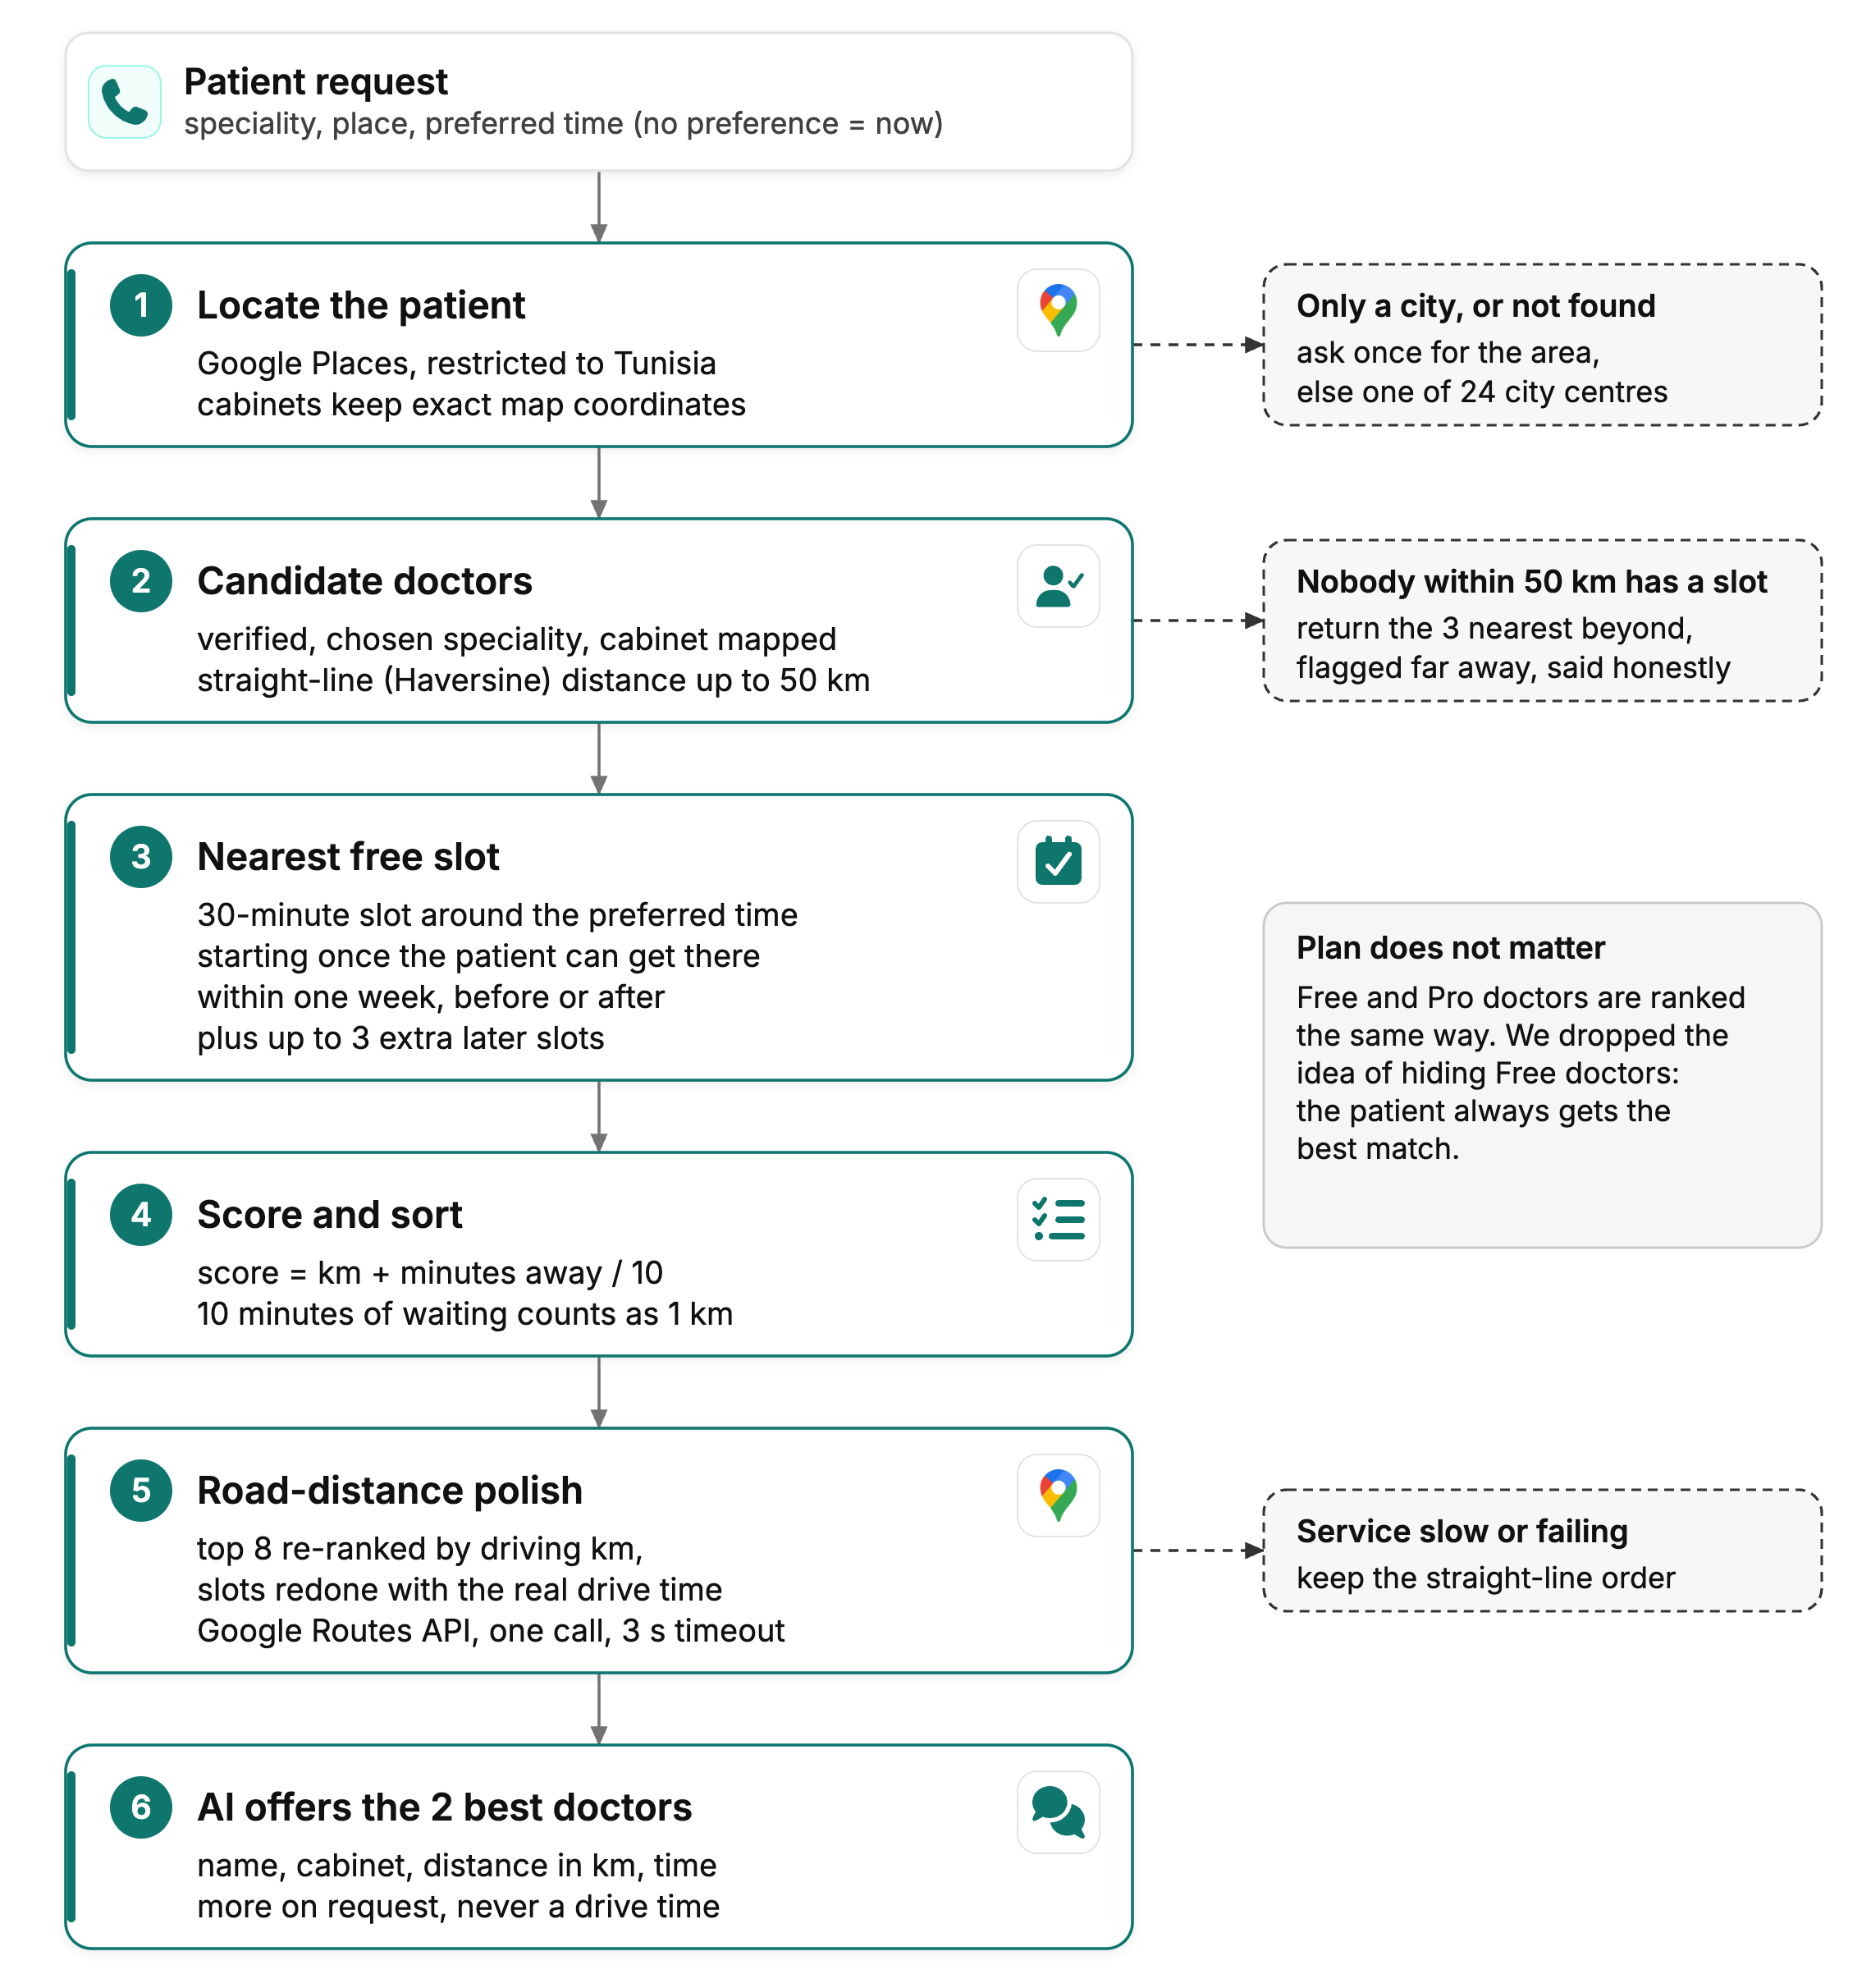
\includegraphics[width=0.85\textwidth,height=0.62\textheight,keepaspectratio]{images/diagrams/bestfit_pipeline.png}
    \caption{The best-fit pipeline, from the patient's request to the 2 or 3 doctors the AI offers}
    \label{fig:bestfit_pipeline}
\end{figure}

\begin{enumerate}
    \item \textbf{Locate the patient.} If this phone line has booked before, the AI first asks whether the patient is in the same area as last time and, if so, reuses that place. Otherwise the place the patient names is looked up with Google Places, restricted to Tunisia. If no precise place is found, the AI falls back to a stored list of 24 Tunisian cities with GPS coordinates. Doctors store the exact coordinates of their cabinet, picked on a map at registration, so the search compares coordinates and not city names.
    \item \textbf{Candidates.} Only verified doctors with the chosen speciality and a mapped cabinet are kept, and doctors that an administrator has excluded from referrals are left out (\secref{subsec:reviews}). Doctors farther than 50~km in a straight line, computed with the Haversine formula, are left out, so a patient in Tunis is not offered a doctor in Sfax. If nobody within 50~km has a free slot, the 3 nearest doctors beyond that limit are returned with a ``far away'' flag, and the AI tells the patient so. Before this fallback, such a search returned nothing.
    \item \textbf{Nearest free slot.} For each doctor, the search finds the free 30-minute slot closest to the preferred time within the next week, before or after it, skipping existing appointments and hours outside the doctor's weekly availability. Up to 3 later slots are kept, so the AI can offer other times without a new search.
    \item \textbf{Score and sort.} Each doctor gets the score below. Lower is better, and 10 minutes of waiting count as much as one kilometre. The time difference is measured against what the patient asked for, not against the current time.
    \item \textbf{Road-distance polish.} The 8 best doctors by straight line are sorted again by driving distance, with one call to the Geoapify Route Matrix and a 3-second timeout. If the service is slow or fails, the straight-line order stays.
    \item \textbf{Answer.} The AI offers the top 2 or 3 doctors with the name, the cabinet address, the distance and the time. It always speaks distance in kilometres, which is how people in Tunisia talk about distance, and never gives a drive time.
\end{enumerate}

\[
\text{score} = \text{distance (km)} + \frac{\lvert \text{slot} - \text{preferred time} \rvert \text{ (minutes)}}{10}
\]

\paragraph{The doctor's plan.} The doctor's plan plays no part in this ranking. When we designed the plans, we considered leaving Free doctors out of the results, so that doctors would have one more reason to subscribe to Pro. We dropped the idea. A patient who calls Riaya should always be offered the doctor who best matches their need, place and time, whatever plan that doctor pays for, and hiding a closer doctor to sell subscriptions would make the service worse for the people it is built for. The plans only limit features on the doctor's side.

\paragraph{Design choices.} A single score lets the search compare a doctor who is close but free later with one who is farther away but free sooner. With 10 minutes of waiting worth one kilometre, a doctor 5~km away at the requested time comes before a doctor next door who is free only one hour later. The 50~km radius keeps the offers to trips that patients would actually make, and the far-away fallback means that a patient in an area with few doctors still gets an answer, with a clear warning about the distance. Road distance comes last and only reorders the 8 best doctors. Our experiment on 78 searches (\secref{subsec:road-distance-experiment}) showed that it changes the best doctor in about one search out of three but never saves more than about 4 minutes of driving. We therefore kept it as a light polish, whose main benefit is that the AI can quote a real road distance.

\paragraph{Prices.} The search does not use prices, and the platform does not show them. We first wanted to, since price matters when choosing a doctor. The price of a first consultation is easy to give, but the real cost depends on what follows, and two doctors with the same consultation price can charge very different amounts for it. Letting doctors enter a price for each service works for services with a fixed price, such as braces. Most patients, though, do not know what they need before a diagnosis, and an AI cannot make that diagnosis over the phone. A partial price could mislead patients, so we left prices out.

\paragraph{Geocoding.} The search is only as good as the patient's position. Callers name neighbourhoods, hospitals, schools and streets, usually in Derja or in French, so we compared several place search services on Tunisian places before choosing Google Places. \secref{subsec:geocoding-evaluation} describes that comparison. Google is not perfect either, and some names exist in several towns, so the AI also gets the list of Tunisian cities and asks the patient to choose when several places match.

\subsection{Urgent Requests and Timeouts}\label{subsec:urgencies}

Some callers are in danger. When a caller describes signs of a life-threatening condition, such as chest pain, trouble breathing, signs of a stroke, heavy bleeding, fainting, a seizure or a serious injury, the AI first tells them to call the SAMU at 190. Riaya books visits and does not replace the emergency services, so the offer of urgent requests to nearby doctors only comes after that advice. For urgent cases that are not life-threatening, the AI asks whether the patient wants the closest available doctors right now. \xref{fig:activity_urgent} in \chapref{chap:management} shows the whole flow.

A patient in an urgent case should not wait 10 minutes for one doctor and then start again. An urgent booking therefore runs the best-fit search with ``now'' as the preferred time and sends up to 3 pending requests at once, all sharing one emergency group id. The first doctor to accept keeps the patient and the other requests of the group are cancelled automatically, so the patient never ends up with several appointments. A doctor who refuses cancels only their own request, since the others can still accept, and for the same reason a refused urgent request triggers no callback. When the patient cancels one urgent request by phone, the whole group is cancelled. If nobody accepts within 10 minutes, a delayed BullMQ job cancels the group and Riaya calls the patient back, as for a normal request. Urgent requests are never limited by a doctor's plan. The delayed jobs and the events between the servers follow the message-based style described by Hohpe and Woolf.

\subsection{Refusals and Callbacks}
\label{subsec:rejection-handling}

We had to decide what happens when a doctor refuses a request or does not answer. Our first idea was to ask the patient for a backup doctor during the call. The call already asks many questions, though, and we wanted to keep it short. So the patient picks one doctor, and if that doctor says no or stays silent, Riaya calls the patient back with new options. After a refusal, Riaya keeps what the patient asked for in Redis for 24 hours, and the AI speaks first in the callback and offers up to 3 other doctors with free slots. If the patient calls Riaya before that, the AI offers these doctors first. After a timeout, the callback only asks the patient to call again. A callback that does not reach the patient is replaced by the same message on WhatsApp from the platform account, and blocked numbers get neither. \xref{fig:bpmn_callback} in \chapref{chap:management} shows the three outcomes of a normal request, and \xref{fig:sequence_callback} shows how the queue, the web app, the voice server and Twilio work together for these callbacks.

\subsection{Patient Reviews and Referral Quality}\label{subsec:reviews}

Two hours after a confirmed visit, a delayed BullMQ job sends the patient a WhatsApp link to the review page (\xref{fig:scr_review}). The job is tied to the appointment. When a doctor moves a confirmed appointment on the calendar, the job is replaced, so the link still arrives two hours after the new end time. When the job runs, it checks again that the appointment is confirmed and that the visit is over.

Each visit can be rated once. A patient who comes often should not get a message after every visit, so no new request goes to a patient who already received one for the same doctor in the last 30 days, whether they answered it or not. A link stops working 30 days after it was sent.

We first built a rating page for doctors and then removed it. Few patients write a comment, a doctor with 30 visits a month collects only a handful of ratings, and a doctor who sees a low score may blame the assistant that booked the patient. The ratings are used by Riaya instead, to decide which doctors the phone assistant keeps offering to callers. Doctors see no rating anywhere.

The Ratings page (\xref{fig:scr_ratings}) shows for each doctor the average rating, the average over the last 90 days, the number of reviews and the share of long waits. Each patient counts once in the average: the ratings of one patient are averaged first, so a patient who comes every week does not set the score alone. Below 5 reviews the values are shown in grey and the doctor is sorted after the doctors with enough reviews. A doctor with an average under 3 over at least 5 reviews is highlighted in red.

The decision stays with the administrator, who opens the doctor's reviews and can stop referrals with a written reason (\xref{fig:scr_rating_detail}). The doctor then disappears from the best-fit search, from urgent requests and from the Best Fit Finder, but keeps the account, the existing appointments and the patients who ask for them by name. We did not lower a doctor's rank automatically from the ratings, because each doctor has too few reviews for such a score to be trusted, and some ratings may judge the booking more than the visit. The excluded doctor sees a banner with the administrator's reason and the support address (\xref{fig:scr_referral_banner}), and no score.

\section{Consultation Recordings}\label{sec:recordings}

A doctor records a consultation in the browser from the Recordings page (\xref{fig:scr_recordings}) and can attach it to a patient. While the recording runs, the browser keeps a copy of the audio in IndexedDB, saved in small pieces, so a closed tab, a refresh or a crash does not lose the consultation. When the doctor stops, the browser uploads the audio straight to Cloudflare R2 with a presigned URL, and the web application saves the recording and processes it in the background.

The audio is transcribed with Microsoft MAI Transcribe 2 through OpenRouter, with speaker separation turned on, so each part of the transcript has a time and a speaker number. The voice model tests ruled this model out for phone calls because it only works on a finished file (\secref{subsec:voice-model-evaluation}), which is exactly what a recording is. The transcriber only numbers the speakers, so a second call, to the chat model (DeepSeek V4 Flash by default), reads the transcript and decides which speaker is the doctor, the patient or a companion. The same call gives the recording a title from what was said, unless the doctor already named it. The doctor can correct the roles if the model got them wrong (\xref{fig:scr_recording}).

On the Pro plan, the chat model then writes a consultation note with five parts: reason for the visit, history, examination, assessment and plan. It writes in French, the usual language of medical records in Tunisia, even when the consultation was in Derja, and keeps drug names and doses as they were said. It only uses what was said and leaves a part empty when it was not discussed, so it never adds a diagnosis or a treatment of its own. The doctor can edit the note or write it again. When the recording is attached to a patient, the note appears in that patient's file, and the AI assistant can read it.

Recording time is counted from the length that the transcriber reports, not from the browser's timer, so a client cannot under-report it. Each recording is charged once, so a retry after a failed transcription is free. When no recording time is left, the recording is still saved, marked as not transcribed, and the doctor can transcribe it later, for example after buying an hour pack.

\section{AI Assistant}\label{sec:assistant}

The assistant is a chat in the doctor's dashboard (\xref{fig:scr_ai_assistant}). It answers medical questions and questions about how to use Riaya, and it works on the practice's own data. Its instructions include a short guide to the dashboard and the plan limits, so it can explain the product as it is. It uses the same chat model as the recordings, through OpenRouter.

The model never reads the database directly. It gets two kinds of tools. The read tools return the schedule between two days, the pending bookings, the patients found by name or CIN, a summary of one patient (appointments, medical files, notes from recordings and unpaid invoices), the free slots of a day, the invoices and the practice statistics. The action tools prepare a change: an invoice, the answer to a pending booking, a note for a medical file, a new appointment or a new time for an existing one. An action tool saves nothing. Its proposal appears as a card that the doctor can edit, then confirm or dismiss, and nothing changes until the doctor confirms. The confirmation calls the same API route as the normal screens, so the usual checks on ownership, overlaps and plan limits apply. The model never invents ids: it gets them from its search tools, and the server checks each one.

A recording can be brought into the chat. The doctor attaches a finished transcript to a question, or opens the assistant from a recording with \textit{Discuss with AI}, and can then ask about the consultation, for example to review the reasoning or draft a summary.

One reply can take up to six model calls, since the model may call a tool, read the result and continue. The reply runs on the server apart from the request: if the doctor closes the page, it still finishes and is saved, and the doctor can stop it at any time. Only the last 20 messages go back to the model with each new question. The use of the assistant is limited by what its replies cost and not by the number of messages (\secref{subsec:usage-limits}), and \secref{sec:security} explains how patient data is kept private.

\section{Evaluations and Tests}\label{sec:evaluations}

Several choices in Riaya depended on how outside services behave with Tunisian places and Tunisian speech, which their documentation does not tell. We therefore tested the options ourselves before settling on them. The comparison of geocoding providers led us to Google Places, the road-distance experiment showed how much the Route Matrix step adds to the best-fit search, and the voice model tests led to Gemini Live. The last subsection explains how the platform as a whole was tested.

\subsection{Geocoding Provider Evaluation}
\label{subsec:geocoding-evaluation}

The first version of the search used Geoapify to find places. Before settling on a provider, we compared several of them on the same Tunisian queries, among them Geoapify, Mapbox and Google Places.

We wrote a list of real places of the kinds patients mention: hospitals, universities, train stations, and the addresses of doctors' cabinets, all written in French, the way most addresses are written in Tunisia. For each place we knew the true position. We sent every query to each provider, restricted to Tunisia, and compared the position it returned with the true one, looking at two things: whether the provider found the place at all, and how far its answer was from the real position.

Google Places was clearly the best. It found many more of the places, including clinics, businesses and smaller institutions that the others did not know, and the positions it returned were more accurate. Geoapify and Mapbox were weaker on both points, so Geoapify was only used for these tests and Google Places became the provider for finding places. The code keeps a switch between the two providers behind one interface, so the rest of the search does not depend on the choice. Google's autocomplete and place details calls share a session token, which counts them as one lookup.

Road distance is a different service. For the polish step of the best-fit search we still use Geoapify's Route Matrix, which returns the driving distances to the 8 candidates in a single call.

\subsection{Road Distance Experiment}
\label{subsec:road-distance-experiment}

Road distance costs a call to an outside service on every search, so we measured whether it changes the result. We ran the search for the 4 specialities with the most doctors, with the patient at the centre of each of the 24 cities, which gave 78 comparisons with no failed call. For each one we took the 8 nearest doctors by straight line and asked for their road distance. \xref{tab:road-distance} shows the results. In one case in Tunis, the nearest doctor was 1.3~km away in a straight line but 5.8~km by road, while another doctor was 2.3~km away both ways; road distance correctly picks the second one. Overall, the best doctor changed in about one search out of three, but the trip saved was small, never more than about 4 minutes. Straight-line distance is therefore a good first filter, and road distance is a light polish whose main benefit is that the AI can quote a real road distance. The test has limits: it used distance only, without appointment times, it placed patients at city centres, it ran on our local data, which may include test doctors, and it only checked the 8 nearest doctors.

\begin{table}[H]
    \centering
    \caption{Effect of road distance on the best doctor (78 searches)}
    \label{tab:road-distance}
    \small
    \begin{tabular}{>{\raggedright\arraybackslash}p{\dimexpr 0.5385\dimexpr\textwidth-4\tabcolsep\relax\relax}>{\raggedright\arraybackslash}p{\dimexpr 0.4615\dimexpr\textwidth-4\tabcolsep\relax\relax}}
        \toprule
        \textbf{Measure} & \textbf{Result} \\
        \midrule
        Best doctor changes (road kilometres) & 24 of 78 (31\%) \\
        Best doctor changes (drive time) & 19 of 78 (24\%) \\
        Time saved when the doctor changes & Median 0.8 min, maximum 4.1 min \\
        Searches saving 5 minutes or more & 0 \\
        Road distance divided by straight distance & Typically 1.01; 1.9 or more for the worst 10\%; 3.27 at worst \\
        \bottomrule
    \end{tabular}
    \\[0.2cm]
\end{table}

\subsection{Voice Model Evaluation and Selection}
\label{subsec:voice-model-evaluation}

The phone call is the reason patients use Riaya, so most of our testing time went into it.

\subsubsection{Two Ways to Build a Phone Call}

In the first approach, called \emph{speech to speech} or realtime, one model listens to the caller and answers with its own voice. It is fast and sounds natural, but the whole conversation depends on one provider. OpenAI Realtime and Gemini Live work this way. The second approach is a \emph{chain of steps}: a speech-to-text model writes down what the caller said, a language model (LLM) writes the answer, and a text-to-speech model reads it out. We could then pick the best model for each step, but every step adds its own wait. We built the chain with LiveKit Agents, which lets us swap the model of each step with a setting. We tested both approaches with the same instructions and the same booking tools.

\subsubsection{Test Method and Its Limits}

We wrote a small program that acts like a phone caller. It plays the same 7 sentences every time, in Tunisian Arabic, in French, and mixed, such as \textit{``\foreignlanguage{arabic}{نحب ناخذ} rendez-vous \foreignlanguage{arabic}{عند} dermatologue''} (``I want to book an appointment with a dermatologist''). It uses the real instructions and booking tools, records what the AI answers, and measures how long each answer takes. We also timed each step of the chain on its own to find where the time went.

To compare engines on full calls, we then built the \texttt{/test-call} page. A tester can call from the browser and choose, for each call, the realtime backend or the model of each step of the chain, plus the model of the caller transcriber. Every option shows our rating, a note, its speed and its price. Only simulated calls read these settings, so real calls always use the server's configuration. The method has a clear limit: the test sentences were spoken by computer voices, not by real patients on real phone lines, and the ratings are our own judgement on a small set of sentences. Prices below come from OpenRouter's model list, checked on 11 October 2026; where we give none, the model runs on another provider.

\subsubsection{The Challenge of Tunisian Arabic}

For English and French, almost every model we tried worked. Tunisian Arabic (Derja) is where they differed, and it was the main problem from the start. Few models understand it. One returned nothing at all for Arabic, and others dropped or misspelled words. Sentences that mix Derja with French words were the hardest: many models wrote the French words in Arabic script, so \textit{dermatologue} came back as an Arabic transliteration that the rest of the system could not match. Few voices speak Derja well either, and several models have no Arabic voice at all. We judged every choice on Tunisian Arabic first, because that is how most patients speak.

\subsubsection{Realtime Models}

\xref{tab:realtime-models} gives our verdicts on the realtime models. OpenAI Realtime was the first one we tested and the smartest of the early tests, but its voice did not have the right accent and it was very expensive. Among the Gemini models, the first versions spoke a good dialect but understood the caller poorly, and the extended-thinking version failed to use the tool results in 8 of 18 tries. \texttt{gemini-3.1-flash-live-preview} was the best of the family. It answered in 1.6 to 4.5 seconds, the longer times when it first had to call a tool.

\begin{table}[H]
    \centering
    \caption{Realtime (speech-to-speech) models tested}
    \label{tab:realtime-models}
    \small
    \begin{tabular}{>{\raggedright\arraybackslash}p{\dimexpr 0.3066\dimexpr\textwidth-6\tabcolsep\relax\relax}>{\raggedright\arraybackslash}p{\dimexpr 0.1387\dimexpr\textwidth-6\tabcolsep\relax\relax}>{\raggedright\arraybackslash}p{\dimexpr 0.5547\dimexpr\textwidth-6\tabcolsep\relax\relax}}
        \toprule
        \textbf{Model} & \textbf{Verdict} & \textbf{What we found} \\
        \midrule
        Gemini Live, \texttt{3.1-flash-live-preview} & Chosen & Tunisian dialect almost perfect, very fast, very good with interruptions, the best reasoning of the Gemini models, understands well. Its own transcript of the caller is very inaccurate. \\
        OpenAI Realtime & Good, not chosen & Fast, good speech recognition, the smartest model of the first tests, very good with interruptions. The voice does not have the right accent, and it is very expensive. \\
        GPT-Live (\texttt{gpt-live-1}) & Bad & Fast, but sounds too artificial, makes mistakes, and the flow is not smooth. Costly, because it runs two models. \\
        \midrule
        \multicolumn{3}{p{14.4cm}}{\textit{Others:} \texttt{gemini-3.8-live} (good dialect and speed, weak understanding), \texttt{gemini-3.8-live} with extended thinking (decent accent, weak understanding, failed to use tool results in 8 of 18 tries), \texttt{gpt-realtime-2.1} (fast, good pronunciation, weak understanding of Arabic and flow), Inworld (about 2.2 s per answer, weak in Arabic, only two Arabic voices).} \\
        \bottomrule
    \end{tabular}
\end{table}

\subsubsection{Speech to Text}

For the chain, the listening step had to handle Derja and keep French words in Latin script. \xref{tab:stt-models} shows the main results. The models that wrote the best text could not stream, so they waited for the end of each sentence before starting. MAI Transcribe 2 gave two different pictures: in the first timed chain it was the best on our sentences, at about 0.5 seconds, but in the later 7-clip run it wrote French words in Arabic script, so we rated it bad for calls. It is still the model that transcribes the doctors' consultation recordings, where it also tells the speakers apart.

\begin{table}[H]
    \centering
    \caption{Main speech-to-text models tested}
    \label{tab:stt-models}
    \small
    \begin{tabular}{>{\raggedright\arraybackslash}p{\dimexpr 0.3066\dimexpr\textwidth-6\tabcolsep\relax\relax}>{\raggedright\arraybackslash}p{\dimexpr 0.1387\dimexpr\textwidth-6\tabcolsep\relax\relax}>{\raggedright\arraybackslash}p{\dimexpr 0.5547\dimexpr\textwidth-6\tabcolsep\relax\relax}}
        \toprule
        \textbf{Model} & \textbf{Verdict} & \textbf{What we found} \\
        \midrule
        Gemini 3 Flash (preview) & Good & Clean French, Derja in Arabic script, French words in Latin script. Slow (about 1.5 s), no streaming. Once wrote a dialogue instead of a transcript. \$0.50 in, \$3.00 out. \\
        \texttt{gemini-3.1-flash-lite} & Pretty good & Fast for a non-streaming model (about 0.8 s), but still too slow for a smooth conversation. Used for the caller transcriber. \$0.25 in, \$1.50 out. \\
        \texttt{gpt-transcribe} & OK & Streams; accepts a list of languages and keywords. Same results as \texttt{gpt-live-transcribe} on the 7 clips. \\
        MAI Transcribe 2 & Bad for calls & Batch only. Turns French words into Arabic script. \\
        Deepgram \texttt{nova-3} & Bad & With an Arabic hint, French and English came back empty; in automatic mode, Derja came back empty. \\
        AssemblyAI Universal & Bad & Not accurate in Arabic, although it keeps French words in Latin script. \\
        \midrule
        \multicolumn{3}{p{14.4cm}}{\textit{Others:} \texttt{gpt-4o-transcribe} and \texttt{gpt-live-transcribe} (bad), \texttt{gemini-3.8-flash} (ok, best on code-switching, waits for each sentence), \texttt{gemini-3.5-flash-lite} (bad, writes Derja in Latin letters), Whisper large v3 turbo, \texttt{gemini-3.5-transcribe}, \texttt{gpt-realtime-whisper}.} \\
        \bottomrule
    \end{tabular}
\end{table}

\subsubsection{Language Model}

The language model of the chain had to follow a long prompt, call the booking tools correctly, and start answering fast. \xref{tab:llm-models} shows what we found. Two numbers come from the timed chain: GPT-5.4 mini started its answer in about 1.2 seconds, and Claude Sonnet, the smartest model we tried, took about 3.6 seconds, three times longer.

\begin{table}[H]
    \centering
    \caption{Main language models tested in the chain}
    \label{tab:llm-models}
    \small
    \begin{tabular}{>{\raggedright\arraybackslash}p{\dimexpr 0.3066\dimexpr\textwidth-6\tabcolsep\relax\relax}>{\raggedright\arraybackslash}p{\dimexpr 0.1387\dimexpr\textwidth-6\tabcolsep\relax\relax}>{\raggedright\arraybackslash}p{\dimexpr 0.5547\dimexpr\textwidth-6\tabcolsep\relax\relax}}
        \toprule
        \textbf{Model} & \textbf{Verdict} & \textbf{What we found} \\
        \midrule
        \texttt{gemini-2.5-flash} & Current & Follows the context well, speed acceptable. The model set in the LiveKit chain today. \$0.30 in, \$2.50 out. \\
        \texttt{gemini-2.5-flash-lite} & Bad & Cheap (\$0.10 in, \$0.40 out) but made too many mistakes in the conversation. \\
        \texttt{gemini-3.8-flash} & Bad & Too slow to answer. \$0.75 in, \$3.75 out. \\
        GPT-5.4 mini & Not kept & The first LLM of the chain; fast to start (about 1.2 s) but less smart than Claude. \$0.75 in, \$4.50 out. \\
        Claude Sonnet and Haiku & Not kept & Sonnet was the smartest but about 3 times slower to start (3.6 s). Haiku was considered and not tried in a call. \\
        \midrule
        \multicolumn{3}{p{14.4cm}}{\textit{Others:} \texttt{gemini-3.1-flash-lite} (set briefly, then replaced), \texttt{gpt-4.1-mini} (considered, not set).} \\
        \bottomrule
    \end{tabular}
\end{table}

\subsubsection{Text to Speech}

For the voice, the problem was the opposite of listening: the voices that spoke real Tunisian Arabic were the slowest, and the fast ones had no Tunisian accent. \xref{tab:tts-models} shows the main results.

\begin{table}[H]
    \centering
    \caption{Main text-to-speech models tested}
    \label{tab:tts-models}
    \small
    \begin{tabular}{>{\raggedright\arraybackslash}p{\dimexpr 0.3066\dimexpr\textwidth-6\tabcolsep\relax\relax}>{\raggedright\arraybackslash}p{\dimexpr 0.1387\dimexpr\textwidth-6\tabcolsep\relax\relax}>{\raggedright\arraybackslash}p{\dimexpr 0.5547\dimexpr\textwidth-6\tabcolsep\relax\relax}}
        \toprule
        \textbf{Model} & \textbf{Verdict} & \textbf{What we found} \\
        \midrule
        Gemini TTS, voice Charon & Best voice, too slow & The flash model has the best voice we heard, with an almost perfect Tunisian dialect, but takes 4 to 5 s. The flash-lite model is very good and takes about 2 s; streamed from Google's API, the first audio came after 0.6 to 1.2 s. \\
        xAI \texttt{tts-1} & Not kept & Very fast (about 0.25 s) and pronounces Arabic, but without a Tunisian accent. \$15 per million characters. \\
        Inworld, voice Omar & Maybe & Fast, used before the switch, but no Tunisian accent and only two Arabic voices. \\
        ElevenLabs \texttt{eleven-v4} & Bad & About 1.5 s, acceptable accent, but very expensive (about \$40 per million characters). \\
        MAI Voice & Bad & Fast (about 0.5 s), but none of its 97 voices is Arabic. \\
        \midrule
        \multicolumn{3}{p{14.4cm}}{\textit{Others:} \texttt{gemini-3.1-flash-tts-preview} (slow, accent not Tunisian), \texttt{gpt-4o-mini-tts} (about 3 s, not streamed), Kokoro, Fish Audio and Deepgram Aura-2 (no Arabic voice).} \\
        \bottomrule
    \end{tabular}
\end{table}

\subsubsection{Lessons Learned}

The best models were often the slowest: the best listening model and the best voice were both slow. In a chain, the delays add up, because the caller waits for every step in turn. \xref{tab:voice-model-comparison} shows the step timings of the chains we measured. The fastest chain we built waited about 6.8 seconds before answering, and with Gemini for both listening and the voice it took more than 10 seconds, far too long for a phone conversation.

\begin{table}[H]
    \centering
    \caption{Speed of each step in the chains we timed}
    \label{tab:voice-model-comparison}
    \small
    \begin{tabular}{>{\raggedright\arraybackslash}p{\dimexpr 0.1571\dimexpr\textwidth-8\tabcolsep\relax\relax}>{\raggedright\arraybackslash}p{\dimexpr 0.2143\dimexpr\textwidth-8\tabcolsep\relax\relax}>{\raggedright\arraybackslash}p{\dimexpr 0.3143\dimexpr\textwidth-8\tabcolsep\relax\relax}>{\raggedright\arraybackslash}p{\dimexpr 0.3143\dimexpr\textwidth-8\tabcolsep\relax\relax}}
        \toprule
        \textbf{Step} & \textbf{Model} & \textbf{What we found} & \textbf{Problem} \\
        \midrule
        Listening & Microsoft MAI & Best on our sentences, about 0.5 s & A preview product with one provider \\
        Listening & Gemini & Excellent text & 2 to 3 s per sentence \\
        Listening & Inworld & Fast & Not good in Arabic, worst on mixed sentences \\
        Thinking & GPT-5.4 mini & Fast, about 1.2 s to start & Less smart than Claude \\
        Thinking & Claude Sonnet & The smartest & 3 times slower to start (3.6 s) \\
        Voice & Gemini & The most natural & 2 to 3 s before it talks \\
        Voice & Inworld & Fast & Only 2 Arabic voices, not perfect \\
        \bottomrule
    \end{tabular}
\end{table}

The tests also found a real bug. The AI saved the caller's name or language on almost every turn, and each save cost about one extra second. In the LiveKit chain we moved this to a background job that reads each caller sentence with a small model and saves the profile without making the caller wait.

\subsubsection{Final Choice}

We chose Gemini Live with the \texttt{gemini-3.1-flash-live-preview} model and the Puck voice. Of all the models we tried, it had the most natural Tunisian dialect, it answered very fast, it handled interruptions very well, and it understood and reasoned best among the Gemini models. OpenAI Realtime was smarter in the first tests, but its accent was wrong for Tunisian callers and it cost much more. GPT-Live sounded too artificial and was also costly, and every chain we built was too slow for a phone call.

Gemini Live's one weakness is its transcript of the caller, which comes from a separate speech-to-text step inside the Live API that we cannot tune. The separate caller transcriber described in \secref{subsec:latency} fixes it for the admin live view and the stored call events. We kept the other realtime backends and the LiveKit chain in the code on purpose, so that new models can be compared again on the test-call page with the same calls.

\subsection{How the Platform Was Tested}

We tested every feature of Riaya, both manually and with AI tools that test every corner of the application. They covered the sign-up and verification steps, the doctor and secretary dashboards, the plans and payments, and the administrator back-office.

Most of the effort went into the phone call, since it is the heart of the product. We first made sure that Twilio worked correctly, with calls to the real number that checked that the phone line reached the assistant on the team's server. Only then did we add the test-call page, to save Twilio's balance: every real call costs money, and a simulated call from the browser costs nothing on Twilio. The page lets us place simulated calls, switch models for each call, and watch the transcript and the tool calls live. The voice server can also send a refusal or timeout callback to an open test-call page instead of placing a real call, so these flows could be tested without Twilio too. We spent a very long time on this page: we made a large number of test calls, compared many models and both approaches described in \secref{subsec:voice-model-evaluation}, and improved the instructions and the booking tools after each round until the assistant handled the calls well.

The comparison of geocoding providers (\secref{subsec:geocoding-evaluation}) and the 78 road-distance comparisons (\secref{subsec:road-distance-experiment}) gave us data for the place search. The admin Best Fit Finder, which runs the same search on a map and a calendar, helped us check the ranking by eye.

The code itself has no automated test suite yet, such as unit tests or end-to-end tests that run on every change. Adding one, starting with the best-fit search, the plan limits and the booking flow, is part of the future work.

\section{Security, Confidentiality, and Access Management}\label{sec:security}

Riaya stores sensitive data: the identity documents that doctors send with their application, patients' medical files, consultation recordings with their transcripts, and recordings of phone calls. This section explains who can reach which data, how the two servers trust each other, and what we did to keep the AI parts and the WhatsApp messages private. It also names the gaps that are still open.

\subsection{Authentication and Authorization}

Accounts are handled by Better Auth with an email and a password. The password needs at least 8 characters, with letters and numbers. At sign-up, Riaya emails a 6-digit code through Nodemailer. The code is valid for 10 minutes and accepts 5 attempts, and a new code can be requested after a 60-second cooldown. These limits follow the usual advice on one-time codes, which is to keep them short-lived and to limit guessing. Until the code is verified, no user row exists. The pending sign-up sits in Better Auth's \texttt{verification} table, with a hash of the code and the password encrypted with AES-256-GCM, and the account is created only when the right code arrives. An address that nobody controls therefore never becomes an account.

An account alone does not make someone a doctor on Riaya. After sign-up the doctor can open only the Profile page, where they fill in an application: CIN pictures (front and back), speciality, Medical Council number and certificate, cabinet name, tax number, and the exact position of the cabinet on a map. An administrator reviews it and approves, rejects with reasons, or bans. Every other dashboard page redirects to Profile until the doctor is verified, so an unverified account cannot receive bookings or see patients.

Authorization is checked on the server for every request. Each API route starts with one of a few helpers: \texttt{requireSession} for any signed-in user, \texttt{requireDoctorProfile} for a verified doctor, \texttt{requirePractice} for routes that a doctor's secretary may also use, \texttt{requireAdmin} for the back office, and \texttt{requireInternal} for calls from the voice server. Hiding a menu item in the interface is never the only protection. Administrators are users whose access level is set in the database; nobody can become one through the sign-up page.

Secretaries are a Pro feature. The doctor invites them by email from the Team page. The link \texttt{/join/<token>} expires after 7 days, can be resent or cancelled, and the database stores only a SHA-256 hash of the token, so a copy of the database does not contain working invitation links. The secretary must sign in with the invited email address. Their access covers the appointments, patients, invoices and availability of that one doctor, without medical files, recordings, the AI assistant or billing. If the doctor drops back to Free or loses verification, the secretary's access is paused, not deleted, and it comes back when Pro is renewed. This follows the principle of least privilege. \xref{tab:auth_matrix} sums up the roles.

\begin{table}[H]
    \centering
    \caption{Authentication and authorization by role}
    \label{tab:auth_matrix}
    \small
    \begin{tabular}{>{\raggedright\arraybackslash}p{\dimexpr 0.1752\dimexpr\textwidth-8\tabcolsep\relax\relax}>{\raggedright\arraybackslash}p{\dimexpr 0.2482\dimexpr\textwidth-8\tabcolsep\relax\relax}>{\raggedright\arraybackslash}p{\dimexpr 0.2847\dimexpr\textwidth-8\tabcolsep\relax\relax}>{\raggedright\arraybackslash}p{\dimexpr 0.2920\dimexpr\textwidth-8\tabcolsep\relax\relax}}
        \toprule
        \textbf{Role} & \textbf{Authentication} & \textbf{Access} & \textbf{Restrictions} \\
        \midrule
        Patient & None; the phone number given by Twilio identifies the line & Phone calls and WhatsApp; a one-time link to rate a doctor & No account and no website; can cancel only pending requests \\
        Doctor & Email and password, email code at sign-up, then admin verification & Full dashboard of their own practice & Profile page only until verified; Pro features need an active Pro plan \\
        Secretary & Email and password, by invitation (link valid 7 days, hashed token) & Appointments, patients, invoices and availability of one doctor & No medical files, recordings, AI assistant, WhatsApp setup or billing; paused when the doctor leaves Pro \\
        Administrator & Email and password; access level set in the database & Back office: applications, live calls and recordings, reports, blocked numbers, users, specialities & Cannot be obtained through sign-up \\
        \bottomrule
    \end{tabular}
\end{table}

\subsection{Protection of Medical Data}

Files are stored in Cloudflare R2. To upload a document, the browser first asks the web app for a presigned URL. This route requires a signed-in user, and the URL it returns is valid for 10 minutes and allows an upload only to a key made of a fixed folder name and a random UUID. The browser then sends the file straight to R2, so medical documents and recordings never pass through our web server, and only the file's link is saved on the record. When a doctor opens a patient, a medical file or a recording, the API first checks on the server that the record belongs to that doctor's practice. Secretaries never receive medical files or recordings, and the AI assistant goes through the same ownership checks for every id it uses.

One weakness remains. The link stored on each record is a public CDN address. The random file names make the links impossible to guess in practice, but anyone who has a link can open the file without signing in, and a link that is forwarded by mistake keeps working. A cleaner design is a private bucket where the API hands out a short-lived signed download link after the same ownership check. We kept this for the future work because it touches every screen that shows a file.

Health data is a sensitive category under the Tunisian law on personal data, and the GDPR is a useful reference for its principles of data minimization and purpose limitation. Riaya keeps little data about patients: no account, no password, and only what the call needs (name, date of birth, gender, address, preferred language), plus the place each phone booking was searched from.

\subsection{Confidentiality of WhatsApp Conversations}

Each doctor links their own WhatsApp account by scanning a QR code on the WhatsApp page. The voice server then sends messages through Baileys from the doctor's own number. Patients see a message from their doctor, and their replies reach the doctor's phone without going through Riaya. Invoices that a secretary sends still leave from the doctor's number. Only system messages, such as the notice that a request expired, come from the platform's own WhatsApp account.

The database has no table for message content. It keeps a monthly counter of the sends a doctor started, for the Free plan limit, and a flag on a medical file once it has been sent. Riaya therefore holds no copy of what doctors and patients write to each other. Baileys works by linking the server as a WhatsApp Web device, so the session keys of each doctor's account live on the voice server. Anyone who controlled that server could send messages as the doctor.

\subsection{Server-to-Server Security}

The voice server calls the web app's internal API to search slots, book, cancel and update a caller's profile. These routes, and the call and person routes the voice server uses, require a shared secret in the \texttt{x-internal-secret} header. The caller's phone number always comes from Twilio and never from the AI, so the model cannot book or cancel for another line, even if a caller tries to make it. The Twilio recording webhook on the web app has to be public, so it checks Twilio's \texttt{X-Twilio-Signature} header (an HMAC-SHA1 of the request) before it accepts a recording. On the voice side, the WebSocket that receives events from the LiveKit agent also requires the shared secret.

Some entry points of the voice server are not protected yet. The \texttt{/incoming-call} webhook does not verify Twilio's signature, and the route the web app uses to send WhatsApp messages, as well as the WebSockets that stream live calls and the WhatsApp QR code, do not check the shared secret or a session. They rely on the voice server's address not being known. Adding the same checks there is one of the first items of the future work.

\subsection{Privacy of the AI Assistant}

The doctor's AI assistant reads patient data, so every chat request it sends to OpenRouter carries two routing options, \texttt{zdr: true} and \texttt{data\_collection: deny}. With them, OpenRouter only uses providers that neither keep nor train on the request. The same options apply to the other chat calls of the web app: recording titles, speaker roles and consultation notes. The two transcription calls, for consultation recordings and for the caller's words on the phone, do not send these options yet, and we plan to add them.

The assistant also cannot change data on its own: every change it prepares waits for the doctor's confirmation and goes through the normal API checks (\secref{sec:assistant}).

\subsection{Abuse Prevention: Reports and Blocked Numbers}

A public phone number attracts abuse. The phone AI gives one calm warning for mockery or insults and calls the \texttt{report\_abuse} tool right away for threats or sexual talk. The prompt tells it never to report confusion, frustration, elderly callers, bad lines, children, jokes, or questions such as ``are you a robot''. When it is not sure, it does not report. It never tells the caller that the call is reported. A report holds a category and a summary written by the AI, and the review page shows it next to the call recording and transcript. Administrators review reports in a queue, and can dismiss one or block the number for 7 days, 30 days or permanently.

Before any AI session starts, the voice server asks the web app whether the caller is blocked. A blocked caller gets a busy signal from Twilio, the attempt is counted, and no recording, callback or WhatsApp message follows. The check has a timeout of about 1.5 seconds and fails open: if the web app is slow or down, the call goes through. We preferred letting an abuser through during an outage to turning away a real patient.
.
% It holds three sections: security and access management, the technical
% challenges with the solutions we adopted, and the evaluations and tests.

\section{Phone Booking}\label{sec:booking}

Phone booking is the main feature of Riaya. This section follows it in the order a patient meets it: the call itself, the search for a doctor, urgent requests, what happens when a doctor refuses or does not answer, and the review after the visit. Each part explains how it works and why we built it that way. The tests behind several of these choices are in \secref{sec:evaluations}.

\subsection{The Call: Latency and Silence Handling}\label{subsec:latency}

During a call, the voice server bridges three WebSocket connections: Twilio's audio stream (G.711 $\mu$-law at 8~kHz), the realtime AI model, and the admin dashboard that shows the live transcript. Every extra millisecond between the caller's last word and the AI's first word makes the call feel less natural. Telephone guidelines aim for a one-way delay of about 150~ms; an AI that has to understand and answer takes far longer, so each step we could remove mattered. The choice of a speech-to-speech model was the biggest gain (\secref{subsec:voice-model-evaluation}). Smaller ones came from the call set-up: the server creates the call row and loads the caller's profile in parallel and caches both, and the check for blocked numbers stops waiting after about 1.5 seconds.

Phone audio is noisy. Before it reaches the model, the caller's audio goes through a high-pass filter that cuts rumble and hum below 250~Hz and a noise gate that follows the background noise level and silences the gaps between words.

Gemini Live understands callers well, but its own transcript of what they said was very inaccurate in our tests, and it cannot be tuned. Since administrators read that transcript in Live Calls and in abuse reports, we added a separate caller transcriber. It splits the caller's audio into sentences with a simple energy check and sends each sentence to \texttt{gemini-3.1-flash-lite} through OpenRouter, which returns it in about 0.8 seconds. It runs beside the conversation, so it does not delay the AI's answers, and it can be turned off with one setting.

Silence was the other problem. Some callers put the phone down without hanging up, and an open call costs money every minute. A shared watchdog, used by the Twilio path and by the LiveKit agent, waits 12 seconds once the assistant is quiet, asks once whether the caller is still there, and says goodbye and hangs up if the caller stays silent for 10 more seconds. Any call ends politely after 15 minutes. Silent calls are logged as a system event and are not treated as abuse.

\subsection{The Best-Fit Search}\label{subsec:bestfit}

While the patient waits on the line, the platform has to turn ``a dermatologist near Ariana tomorrow morning'' into two or three concrete offers. \xref{fig:bestfit_pipeline} shows the six steps of the search.

\begin{figure}[H]
    \centering
    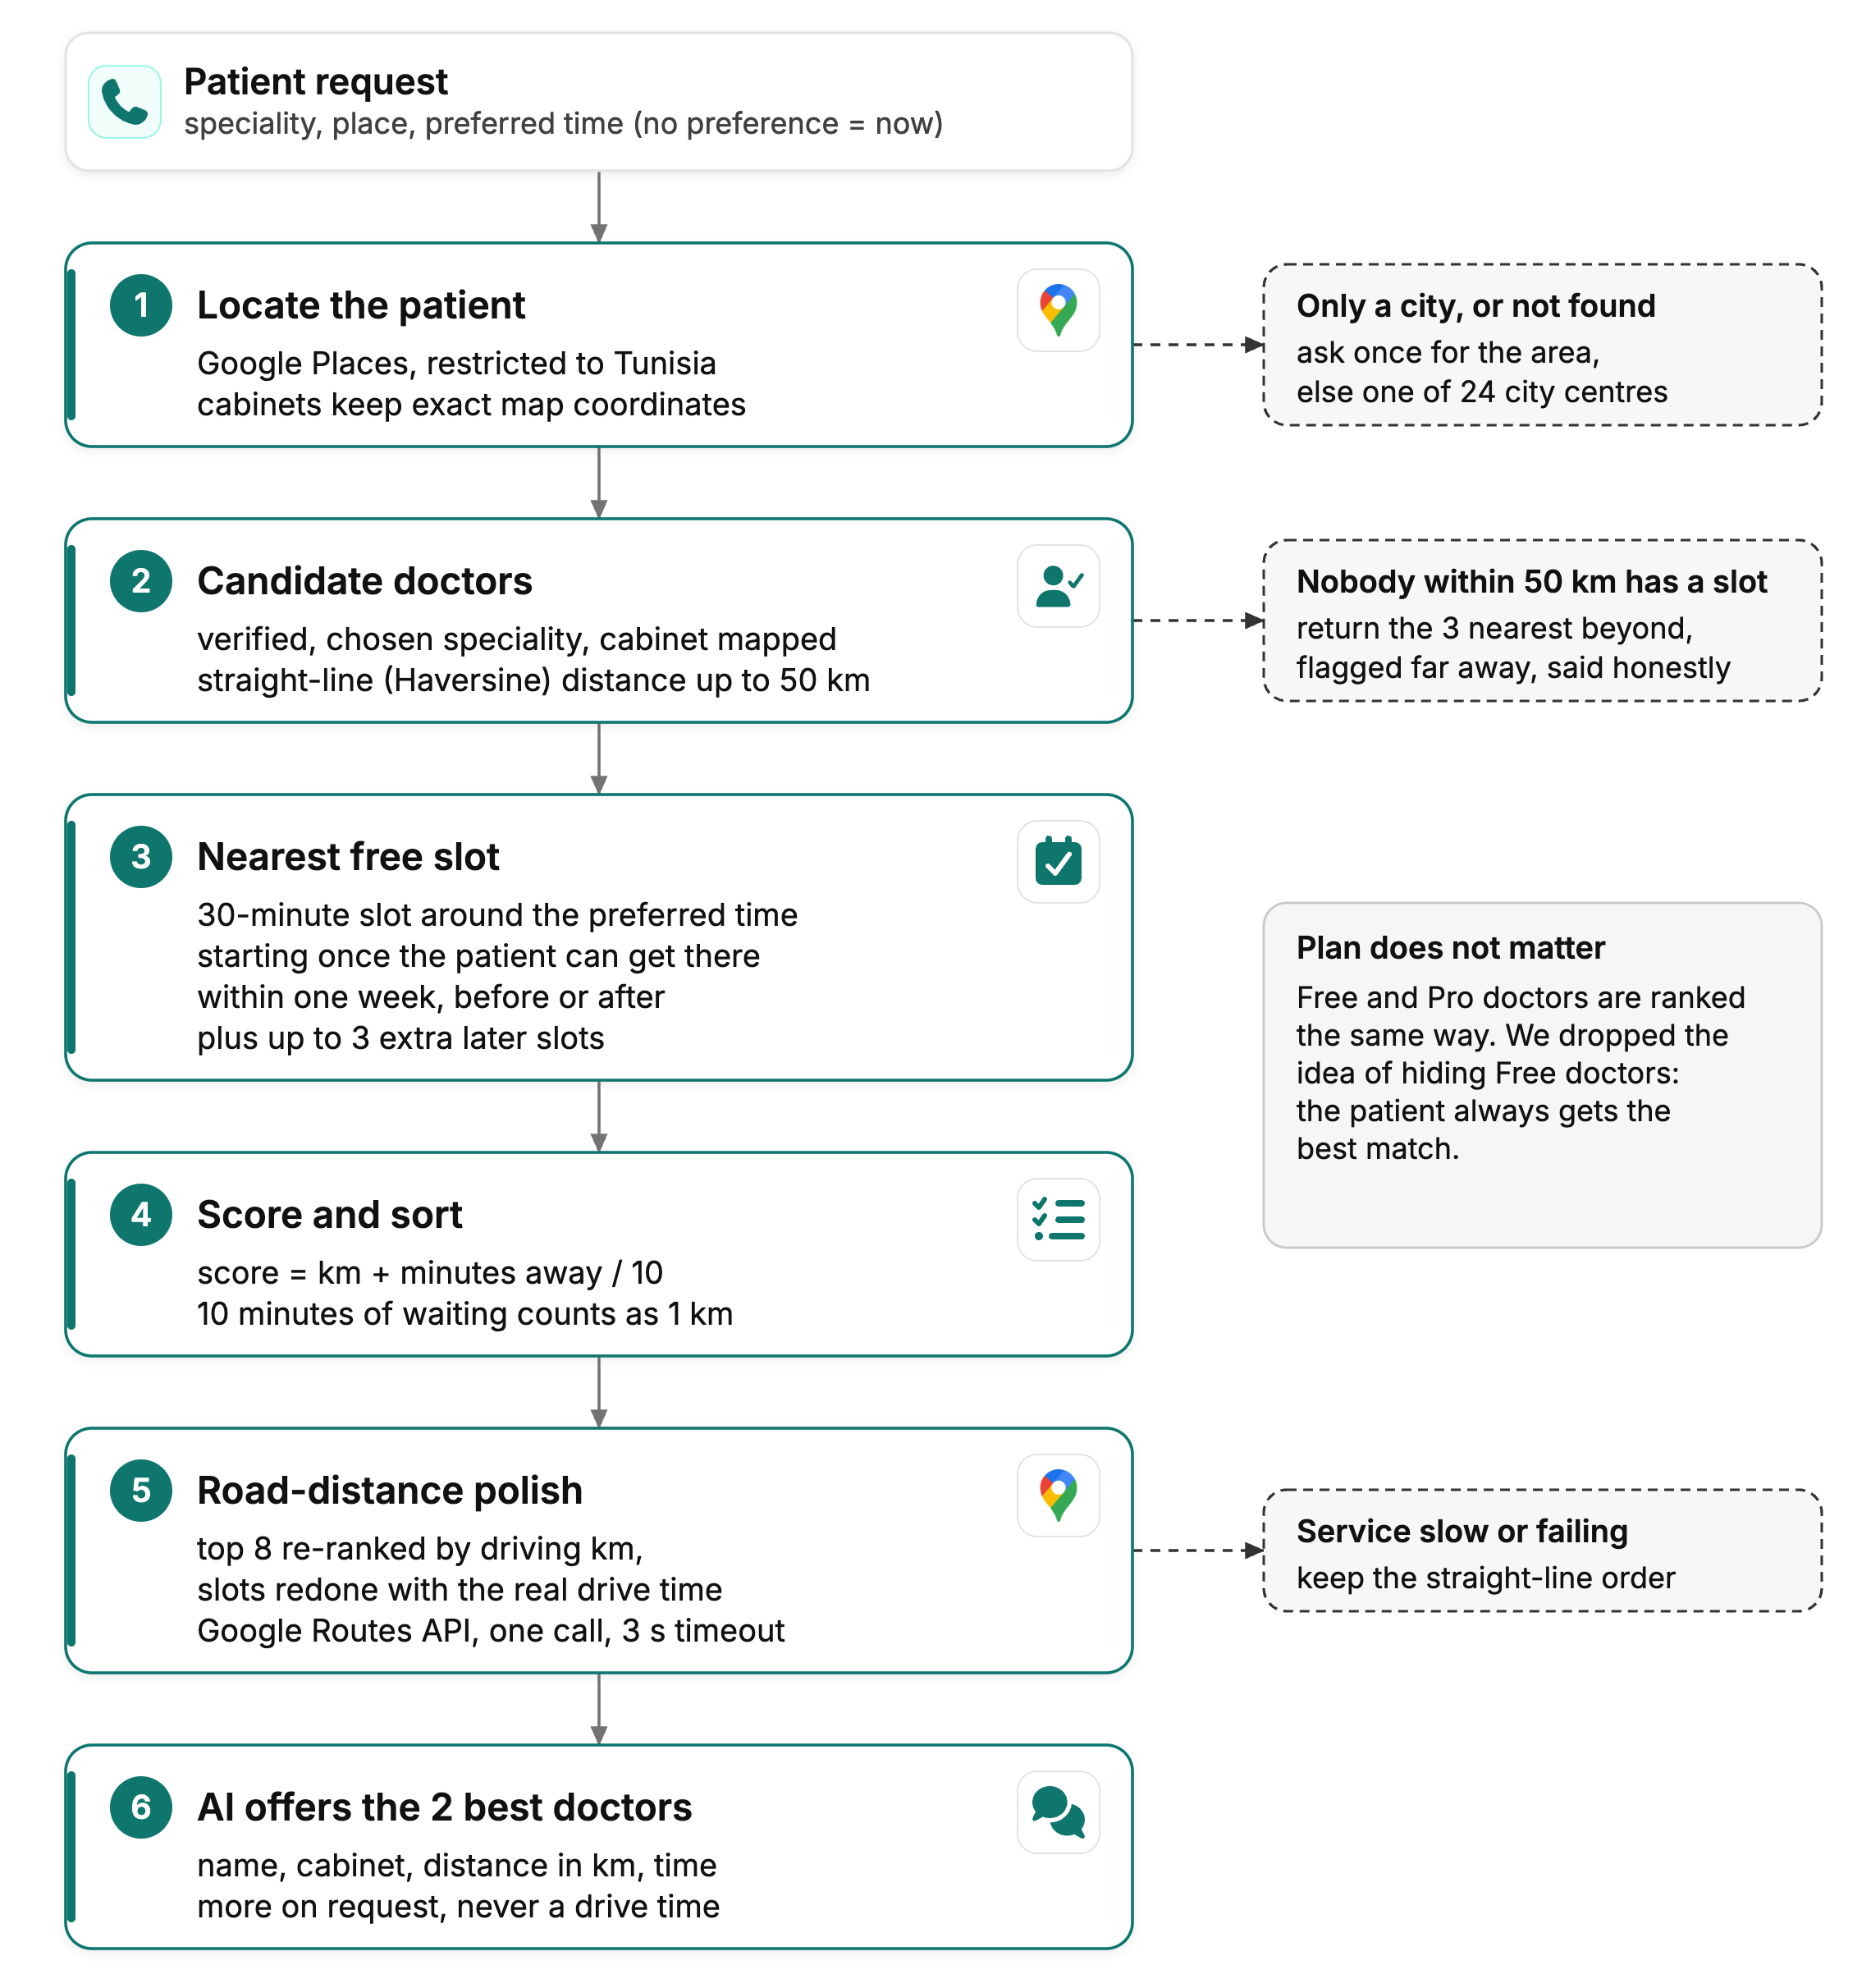
\includegraphics[width=0.85\textwidth,height=0.62\textheight,keepaspectratio]{images/diagrams/bestfit_pipeline.png}
    \caption{The best-fit pipeline, from the patient's request to the 2 or 3 doctors the AI offers}
    \label{fig:bestfit_pipeline}
\end{figure}

\begin{enumerate}
    \item \textbf{Locate the patient.} If this phone line has booked before, the AI first asks whether the patient is in the same area as last time and, if so, reuses that place. Otherwise the place the patient names is looked up with Google Places, restricted to Tunisia. If no precise place is found, the AI falls back to a stored list of 24 Tunisian cities with GPS coordinates. Doctors store the exact coordinates of their cabinet, picked on a map at registration, so the search compares coordinates and not city names.
    \item \textbf{Candidates.} Only verified doctors with the chosen speciality and a mapped cabinet are kept, and doctors that an administrator has excluded from referrals are left out (\secref{subsec:reviews}). Doctors farther than 50~km in a straight line, computed with the Haversine formula, are left out, so a patient in Tunis is not offered a doctor in Sfax. If nobody within 50~km has a free slot, the 3 nearest doctors beyond that limit are returned with a ``far away'' flag, and the AI tells the patient so. Before this fallback, such a search returned nothing.
    \item \textbf{Nearest free slot.} For each doctor, the search finds the free 30-minute slot closest to the preferred time within the next week, before or after it, skipping existing appointments and hours outside the doctor's weekly availability. Up to 3 later slots are kept, so the AI can offer other times without a new search.
    \item \textbf{Score and sort.} Each doctor gets the score below. Lower is better, and 10 minutes of waiting count as much as one kilometre. The time difference is measured against what the patient asked for, not against the current time.
    \item \textbf{Road-distance polish.} The 8 best doctors by straight line are sorted again by driving distance, with one call to the Geoapify Route Matrix and a 3-second timeout. If the service is slow or fails, the straight-line order stays.
    \item \textbf{Answer.} The AI offers the top 2 or 3 doctors with the name, the cabinet address, the distance and the time. It always speaks distance in kilometres, which is how people in Tunisia talk about distance, and never gives a drive time.
\end{enumerate}

\[
\text{score} = \text{distance (km)} + \frac{\lvert \text{slot} - \text{preferred time} \rvert \text{ (minutes)}}{10}
\]

\paragraph{The doctor's plan.} The doctor's plan plays no part in this ranking. When we designed the plans, we considered leaving Free doctors out of the results, so that doctors would have one more reason to subscribe to Pro. We dropped the idea. A patient who calls Riaya should always be offered the doctor who best matches their need, place and time, whatever plan that doctor pays for, and hiding a closer doctor to sell subscriptions would make the service worse for the people it is built for. The plans only limit features on the doctor's side.

\paragraph{Design choices.} A single score lets the search compare a doctor who is close but free later with one who is farther away but free sooner. With 10 minutes of waiting worth one kilometre, a doctor 5~km away at the requested time comes before a doctor next door who is free only one hour later. The 50~km radius keeps the offers to trips that patients would actually make, and the far-away fallback means that a patient in an area with few doctors still gets an answer, with a clear warning about the distance. Road distance comes last and only reorders the 8 best doctors. Our experiment on 78 searches (\secref{subsec:road-distance-experiment}) showed that it changes the best doctor in about one search out of three but never saves more than about 4 minutes of driving. We therefore kept it as a light polish, whose main benefit is that the AI can quote a real road distance.

\paragraph{Prices.} The search does not use prices, and the platform does not show them. We first wanted to, since price matters when choosing a doctor. The price of a first consultation is easy to give, but the real cost depends on what follows, and two doctors with the same consultation price can charge very different amounts for it. Letting doctors enter a price for each service works for services with a fixed price, such as braces. Most patients, though, do not know what they need before a diagnosis, and an AI cannot make that diagnosis over the phone. A partial price could mislead patients, so we left prices out.

\paragraph{Geocoding.} The search is only as good as the patient's position. Callers name neighbourhoods, hospitals, schools and streets, usually in Derja or in French, so we compared several place search services on Tunisian places before choosing Google Places. \secref{subsec:geocoding-evaluation} describes that comparison. Google is not perfect either, and some names exist in several towns, so the AI also gets the list of Tunisian cities and asks the patient to choose when several places match.

\subsection{Urgent Requests and Timeouts}\label{subsec:urgencies}

Some callers are in danger. When a caller describes signs of a life-threatening condition, such as chest pain, trouble breathing, signs of a stroke, heavy bleeding, fainting, a seizure or a serious injury, the AI first tells them to call the SAMU at 190. Riaya books visits and does not replace the emergency services, so the offer of urgent requests to nearby doctors only comes after that advice. For urgent cases that are not life-threatening, the AI asks whether the patient wants the closest available doctors right now. \xref{fig:activity_urgent} in \chapref{chap:management} shows the whole flow.

A patient in an urgent case should not wait 10 minutes for one doctor and then start again. An urgent booking therefore runs the best-fit search with ``now'' as the preferred time and sends up to 3 pending requests at once, all sharing one emergency group id. The first doctor to accept keeps the patient and the other requests of the group are cancelled automatically, so the patient never ends up with several appointments. A doctor who refuses cancels only their own request, since the others can still accept, and for the same reason a refused urgent request triggers no callback. When the patient cancels one urgent request by phone, the whole group is cancelled. If nobody accepts within 10 minutes, a delayed BullMQ job cancels the group and Riaya calls the patient back, as for a normal request. Urgent requests are never limited by a doctor's plan. The delayed jobs and the events between the servers follow the message-based style described by Hohpe and Woolf.

\subsection{Refusals and Callbacks}
\label{subsec:rejection-handling}

We had to decide what happens when a doctor refuses a request or does not answer. Our first idea was to ask the patient for a backup doctor during the call. The call already asks many questions, though, and we wanted to keep it short. So the patient picks one doctor, and if that doctor says no or stays silent, Riaya calls the patient back with new options. After a refusal, Riaya keeps what the patient asked for in Redis for 24 hours, and the AI speaks first in the callback and offers up to 3 other doctors with free slots. If the patient calls Riaya before that, the AI offers these doctors first. After a timeout, the callback only asks the patient to call again. A callback that does not reach the patient is replaced by the same message on WhatsApp from the platform account, and blocked numbers get neither. \xref{fig:bpmn_callback} in \chapref{chap:management} shows the three outcomes of a normal request, and \xref{fig:sequence_callback} shows how the queue, the web app, the voice server and Twilio work together for these callbacks.

\subsection{Patient Reviews and Referral Quality}\label{subsec:reviews}

Two hours after a confirmed visit, a delayed BullMQ job sends the patient a WhatsApp link to the review page (\xref{fig:scr_review}). The job is tied to the appointment. When a doctor moves a confirmed appointment on the calendar, the job is replaced, so the link still arrives two hours after the new end time. When the job runs, it checks again that the appointment is confirmed and that the visit is over.

Each visit can be rated once. A patient who comes often should not get a message after every visit, so no new request goes to a patient who already received one for the same doctor in the last 30 days, whether they answered it or not. A link stops working 30 days after it was sent.

We first built a rating page for doctors and then removed it. Few patients write a comment, a doctor with 30 visits a month collects only a handful of ratings, and a doctor who sees a low score may blame the assistant that booked the patient. The ratings are used by Riaya instead, to decide which doctors the phone assistant keeps offering to callers. Doctors see no rating anywhere.

The Ratings page (\xref{fig:scr_ratings}) shows for each doctor the average rating, the average over the last 90 days, the number of reviews and the share of long waits. Each patient counts once in the average: the ratings of one patient are averaged first, so a patient who comes every week does not set the score alone. Below 5 reviews the values are shown in grey and the doctor is sorted after the doctors with enough reviews. A doctor with an average under 3 over at least 5 reviews is highlighted in red.

The decision stays with the administrator, who opens the doctor's reviews and can stop referrals with a written reason (\xref{fig:scr_rating_detail}). The doctor then disappears from the best-fit search, from urgent requests and from the Best Fit Finder, but keeps the account, the existing appointments and the patients who ask for them by name. We did not lower a doctor's rank automatically from the ratings, because each doctor has too few reviews for such a score to be trusted, and some ratings may judge the booking more than the visit. The excluded doctor sees a banner with the administrator's reason and the support address (\xref{fig:scr_referral_banner}), and no score.

\section{Consultation Recordings}\label{sec:recordings}

A doctor records a consultation in the browser from the Recordings page (\xref{fig:scr_recordings}) and can attach it to a patient. While the recording runs, the browser keeps a copy of the audio in IndexedDB, saved in small pieces, so a closed tab, a refresh or a crash does not lose the consultation. When the doctor stops, the browser uploads the audio straight to Cloudflare R2 with a presigned URL, and the web application saves the recording and processes it in the background.

The audio is transcribed with Microsoft MAI Transcribe 2 through OpenRouter, with speaker separation turned on, so each part of the transcript has a time and a speaker number. The voice model tests ruled this model out for phone calls because it only works on a finished file (\secref{subsec:voice-model-evaluation}), which is exactly what a recording is. The transcriber only numbers the speakers, so a second call, to the chat model (DeepSeek V4 Flash by default), reads the transcript and decides which speaker is the doctor, the patient or a companion. The same call gives the recording a title from what was said, unless the doctor already named it. The doctor can correct the roles if the model got them wrong (\xref{fig:scr_recording}).

On the Pro plan, the chat model then writes a consultation note with five parts: reason for the visit, history, examination, assessment and plan. It writes in French, the usual language of medical records in Tunisia, even when the consultation was in Derja, and keeps drug names and doses as they were said. It only uses what was said and leaves a part empty when it was not discussed, so it never adds a diagnosis or a treatment of its own. The doctor can edit the note or write it again. When the recording is attached to a patient, the note appears in that patient's file, and the AI assistant can read it.

Recording time is counted from the length that the transcriber reports, not from the browser's timer, so a client cannot under-report it. Each recording is charged once, so a retry after a failed transcription is free. When no recording time is left, the recording is still saved, marked as not transcribed, and the doctor can transcribe it later, for example after buying an hour pack.

\section{AI Assistant}\label{sec:assistant}

The assistant is a chat in the doctor's dashboard (\xref{fig:scr_ai_assistant}). It answers medical questions and questions about how to use Riaya, and it works on the practice's own data. Its instructions include a short guide to the dashboard and the plan limits, so it can explain the product as it is. It uses the same chat model as the recordings, through OpenRouter.

The model never reads the database directly. It gets two kinds of tools. The read tools return the schedule between two days, the pending bookings, the patients found by name or CIN, a summary of one patient (appointments, medical files, notes from recordings and unpaid invoices), the free slots of a day, the invoices and the practice statistics. The action tools prepare a change: an invoice, the answer to a pending booking, a note for a medical file, a new appointment or a new time for an existing one. An action tool saves nothing. Its proposal appears as a card that the doctor can edit, then confirm or dismiss, and nothing changes until the doctor confirms. The confirmation calls the same API route as the normal screens, so the usual checks on ownership, overlaps and plan limits apply. The model never invents ids: it gets them from its search tools, and the server checks each one.

A recording can be brought into the chat. The doctor attaches a finished transcript to a question, or opens the assistant from a recording with \textit{Discuss with AI}, and can then ask about the consultation, for example to review the reasoning or draft a summary.

One reply can take up to six model calls, since the model may call a tool, read the result and continue. The reply runs on the server apart from the request: if the doctor closes the page, it still finishes and is saved, and the doctor can stop it at any time. Only the last 20 messages go back to the model with each new question. The use of the assistant is limited by what its replies cost and not by the number of messages (\secref{subsec:usage-limits}), and \secref{sec:security} explains how patient data is kept private.

\section{Evaluations and Tests}\label{sec:evaluations}

Several choices in Riaya depended on how outside services behave with Tunisian places and Tunisian speech, which their documentation does not tell. We therefore tested the options ourselves before settling on them. The comparison of geocoding providers led us to Google Places, the road-distance experiment showed how much the Route Matrix step adds to the best-fit search, and the voice model tests led to Gemini Live. The last subsection explains how the platform as a whole was tested.

\subsection{Geocoding Provider Evaluation}
\label{subsec:geocoding-evaluation}

The first version of the search used Geoapify to find places. Before settling on a provider, we compared several of them on the same Tunisian queries, among them Geoapify, Mapbox and Google Places.

We wrote a list of real places of the kinds patients mention: hospitals, universities, train stations, and the addresses of doctors' cabinets, all written in French, the way most addresses are written in Tunisia. For each place we knew the true position. We sent every query to each provider, restricted to Tunisia, and compared the position it returned with the true one, looking at two things: whether the provider found the place at all, and how far its answer was from the real position.

Google Places was clearly the best. It found many more of the places, including clinics, businesses and smaller institutions that the others did not know, and the positions it returned were more accurate. Geoapify and Mapbox were weaker on both points, so Geoapify was only used for these tests and Google Places became the provider for finding places. The code keeps a switch between the two providers behind one interface, so the rest of the search does not depend on the choice. Google's autocomplete and place details calls share a session token, which counts them as one lookup.

Road distance is a different service. For the polish step of the best-fit search we still use Geoapify's Route Matrix, which returns the driving distances to the 8 candidates in a single call.

\subsection{Road Distance Experiment}
\label{subsec:road-distance-experiment}

Road distance costs a call to an outside service on every search, so we measured whether it changes the result. We ran the search for the 4 specialities with the most doctors, with the patient at the centre of each of the 24 cities, which gave 78 comparisons with no failed call. For each one we took the 8 nearest doctors by straight line and asked for their road distance. \xref{tab:road-distance} shows the results. In one case in Tunis, the nearest doctor was 1.3~km away in a straight line but 5.8~km by road, while another doctor was 2.3~km away both ways; road distance correctly picks the second one. Overall, the best doctor changed in about one search out of three, but the trip saved was small, never more than about 4 minutes. Straight-line distance is therefore a good first filter, and road distance is a light polish whose main benefit is that the AI can quote a real road distance. The test has limits: it used distance only, without appointment times, it placed patients at city centres, it ran on our local data, which may include test doctors, and it only checked the 8 nearest doctors.

\begin{table}[H]
    \centering
    \caption{Effect of road distance on the best doctor (78 searches)}
    \label{tab:road-distance}
    \small
    \begin{tabular}{>{\raggedright\arraybackslash}p{\dimexpr 0.5385\dimexpr\textwidth-4\tabcolsep\relax\relax}>{\raggedright\arraybackslash}p{\dimexpr 0.4615\dimexpr\textwidth-4\tabcolsep\relax\relax}}
        \toprule
        \textbf{Measure} & \textbf{Result} \\
        \midrule
        Best doctor changes (road kilometres) & 24 of 78 (31\%) \\
        Best doctor changes (drive time) & 19 of 78 (24\%) \\
        Time saved when the doctor changes & Median 0.8 min, maximum 4.1 min \\
        Searches saving 5 minutes or more & 0 \\
        Road distance divided by straight distance & Typically 1.01; 1.9 or more for the worst 10\%; 3.27 at worst \\
        \bottomrule
    \end{tabular}
    \\[0.2cm]
\end{table}

\subsection{Voice Model Evaluation and Selection}
\label{subsec:voice-model-evaluation}

The phone call is the reason patients use Riaya, so most of our testing time went into it.

\subsubsection{Two Ways to Build a Phone Call}

In the first approach, called \emph{speech to speech} or realtime, one model listens to the caller and answers with its own voice. It is fast and sounds natural, but the whole conversation depends on one provider. OpenAI Realtime and Gemini Live work this way. The second approach is a \emph{chain of steps}: a speech-to-text model writes down what the caller said, a language model (LLM) writes the answer, and a text-to-speech model reads it out. We could then pick the best model for each step, but every step adds its own wait. We built the chain with LiveKit Agents, which lets us swap the model of each step with a setting. We tested both approaches with the same instructions and the same booking tools.

\subsubsection{Test Method and Its Limits}

We wrote a small program that acts like a phone caller. It plays the same 7 sentences every time, in Tunisian Arabic, in French, and mixed, such as \textit{``\foreignlanguage{arabic}{نحب ناخذ} rendez-vous \foreignlanguage{arabic}{عند} dermatologue''} (``I want to book an appointment with a dermatologist''). It uses the real instructions and booking tools, records what the AI answers, and measures how long each answer takes. We also timed each step of the chain on its own to find where the time went.

To compare engines on full calls, we then built the \texttt{/test-call} page. A tester can call from the browser and choose, for each call, the realtime backend or the model of each step of the chain, plus the model of the caller transcriber. Every option shows our rating, a note, its speed and its price. Only simulated calls read these settings, so real calls always use the server's configuration. The method has a clear limit: the test sentences were spoken by computer voices, not by real patients on real phone lines, and the ratings are our own judgement on a small set of sentences. Prices below come from OpenRouter's model list, checked on 11 October 2026; where we give none, the model runs on another provider.

\subsubsection{The Challenge of Tunisian Arabic}

For English and French, almost every model we tried worked. Tunisian Arabic (Derja) is where they differed, and it was the main problem from the start. Few models understand it. One returned nothing at all for Arabic, and others dropped or misspelled words. Sentences that mix Derja with French words were the hardest: many models wrote the French words in Arabic script, so \textit{dermatologue} came back as an Arabic transliteration that the rest of the system could not match. Few voices speak Derja well either, and several models have no Arabic voice at all. We judged every choice on Tunisian Arabic first, because that is how most patients speak.

\subsubsection{Realtime Models}

\xref{tab:realtime-models} gives our verdicts on the realtime models. OpenAI Realtime was the first one we tested and the smartest of the early tests, but its voice did not have the right accent and it was very expensive. Among the Gemini models, the first versions spoke a good dialect but understood the caller poorly, and the extended-thinking version failed to use the tool results in 8 of 18 tries. \texttt{gemini-3.1-flash-live-preview} was the best of the family. It answered in 1.6 to 4.5 seconds, the longer times when it first had to call a tool.

\begin{table}[H]
    \centering
    \caption{Realtime (speech-to-speech) models tested}
    \label{tab:realtime-models}
    \small
    \begin{tabular}{>{\raggedright\arraybackslash}p{\dimexpr 0.3066\dimexpr\textwidth-6\tabcolsep\relax\relax}>{\raggedright\arraybackslash}p{\dimexpr 0.1387\dimexpr\textwidth-6\tabcolsep\relax\relax}>{\raggedright\arraybackslash}p{\dimexpr 0.5547\dimexpr\textwidth-6\tabcolsep\relax\relax}}
        \toprule
        \textbf{Model} & \textbf{Verdict} & \textbf{What we found} \\
        \midrule
        Gemini Live, \texttt{3.1-flash-live-preview} & Chosen & Tunisian dialect almost perfect, very fast, very good with interruptions, the best reasoning of the Gemini models, understands well. Its own transcript of the caller is very inaccurate. \\
        OpenAI Realtime & Good, not chosen & Fast, good speech recognition, the smartest model of the first tests, very good with interruptions. The voice does not have the right accent, and it is very expensive. \\
        GPT-Live (\texttt{gpt-live-1}) & Bad & Fast, but sounds too artificial, makes mistakes, and the flow is not smooth. Costly, because it runs two models. \\
        \midrule
        \multicolumn{3}{p{14.4cm}}{\textit{Others:} \texttt{gemini-3.8-live} (good dialect and speed, weak understanding), \texttt{gemini-3.8-live} with extended thinking (decent accent, weak understanding, failed to use tool results in 8 of 18 tries), \texttt{gpt-realtime-2.1} (fast, good pronunciation, weak understanding of Arabic and flow), Inworld (about 2.2 s per answer, weak in Arabic, only two Arabic voices).} \\
        \bottomrule
    \end{tabular}
\end{table}

\subsubsection{Speech to Text}

For the chain, the listening step had to handle Derja and keep French words in Latin script. \xref{tab:stt-models} shows the main results. The models that wrote the best text could not stream, so they waited for the end of each sentence before starting. MAI Transcribe 2 gave two different pictures: in the first timed chain it was the best on our sentences, at about 0.5 seconds, but in the later 7-clip run it wrote French words in Arabic script, so we rated it bad for calls. It is still the model that transcribes the doctors' consultation recordings, where it also tells the speakers apart.

\begin{table}[H]
    \centering
    \caption{Main speech-to-text models tested}
    \label{tab:stt-models}
    \small
    \begin{tabular}{>{\raggedright\arraybackslash}p{\dimexpr 0.3066\dimexpr\textwidth-6\tabcolsep\relax\relax}>{\raggedright\arraybackslash}p{\dimexpr 0.1387\dimexpr\textwidth-6\tabcolsep\relax\relax}>{\raggedright\arraybackslash}p{\dimexpr 0.5547\dimexpr\textwidth-6\tabcolsep\relax\relax}}
        \toprule
        \textbf{Model} & \textbf{Verdict} & \textbf{What we found} \\
        \midrule
        Gemini 3 Flash (preview) & Good & Clean French, Derja in Arabic script, French words in Latin script. Slow (about 1.5 s), no streaming. Once wrote a dialogue instead of a transcript. \$0.50 in, \$3.00 out. \\
        \texttt{gemini-3.1-flash-lite} & Pretty good & Fast for a non-streaming model (about 0.8 s), but still too slow for a smooth conversation. Used for the caller transcriber. \$0.25 in, \$1.50 out. \\
        \texttt{gpt-transcribe} & OK & Streams; accepts a list of languages and keywords. Same results as \texttt{gpt-live-transcribe} on the 7 clips. \\
        MAI Transcribe 2 & Bad for calls & Batch only. Turns French words into Arabic script. \\
        Deepgram \texttt{nova-3} & Bad & With an Arabic hint, French and English came back empty; in automatic mode, Derja came back empty. \\
        AssemblyAI Universal & Bad & Not accurate in Arabic, although it keeps French words in Latin script. \\
        \midrule
        \multicolumn{3}{p{14.4cm}}{\textit{Others:} \texttt{gpt-4o-transcribe} and \texttt{gpt-live-transcribe} (bad), \texttt{gemini-3.8-flash} (ok, best on code-switching, waits for each sentence), \texttt{gemini-3.5-flash-lite} (bad, writes Derja in Latin letters), Whisper large v3 turbo, \texttt{gemini-3.5-transcribe}, \texttt{gpt-realtime-whisper}.} \\
        \bottomrule
    \end{tabular}
\end{table}

\subsubsection{Language Model}

The language model of the chain had to follow a long prompt, call the booking tools correctly, and start answering fast. \xref{tab:llm-models} shows what we found. Two numbers come from the timed chain: GPT-5.4 mini started its answer in about 1.2 seconds, and Claude Sonnet, the smartest model we tried, took about 3.6 seconds, three times longer.

\begin{table}[H]
    \centering
    \caption{Main language models tested in the chain}
    \label{tab:llm-models}
    \small
    \begin{tabular}{>{\raggedright\arraybackslash}p{\dimexpr 0.3066\dimexpr\textwidth-6\tabcolsep\relax\relax}>{\raggedright\arraybackslash}p{\dimexpr 0.1387\dimexpr\textwidth-6\tabcolsep\relax\relax}>{\raggedright\arraybackslash}p{\dimexpr 0.5547\dimexpr\textwidth-6\tabcolsep\relax\relax}}
        \toprule
        \textbf{Model} & \textbf{Verdict} & \textbf{What we found} \\
        \midrule
        \texttt{gemini-2.5-flash} & Current & Follows the context well, speed acceptable. The model set in the LiveKit chain today. \$0.30 in, \$2.50 out. \\
        \texttt{gemini-2.5-flash-lite} & Bad & Cheap (\$0.10 in, \$0.40 out) but made too many mistakes in the conversation. \\
        \texttt{gemini-3.8-flash} & Bad & Too slow to answer. \$0.75 in, \$3.75 out. \\
        GPT-5.4 mini & Not kept & The first LLM of the chain; fast to start (about 1.2 s) but less smart than Claude. \$0.75 in, \$4.50 out. \\
        Claude Sonnet and Haiku & Not kept & Sonnet was the smartest but about 3 times slower to start (3.6 s). Haiku was considered and not tried in a call. \\
        \midrule
        \multicolumn{3}{p{14.4cm}}{\textit{Others:} \texttt{gemini-3.1-flash-lite} (set briefly, then replaced), \texttt{gpt-4.1-mini} (considered, not set).} \\
        \bottomrule
    \end{tabular}
\end{table}

\subsubsection{Text to Speech}

For the voice, the problem was the opposite of listening: the voices that spoke real Tunisian Arabic were the slowest, and the fast ones had no Tunisian accent. \xref{tab:tts-models} shows the main results.

\begin{table}[H]
    \centering
    \caption{Main text-to-speech models tested}
    \label{tab:tts-models}
    \small
    \begin{tabular}{>{\raggedright\arraybackslash}p{\dimexpr 0.3066\dimexpr\textwidth-6\tabcolsep\relax\relax}>{\raggedright\arraybackslash}p{\dimexpr 0.1387\dimexpr\textwidth-6\tabcolsep\relax\relax}>{\raggedright\arraybackslash}p{\dimexpr 0.5547\dimexpr\textwidth-6\tabcolsep\relax\relax}}
        \toprule
        \textbf{Model} & \textbf{Verdict} & \textbf{What we found} \\
        \midrule
        Gemini TTS, voice Charon & Best voice, too slow & The flash model has the best voice we heard, with an almost perfect Tunisian dialect, but takes 4 to 5 s. The flash-lite model is very good and takes about 2 s; streamed from Google's API, the first audio came after 0.6 to 1.2 s. \\
        xAI \texttt{tts-1} & Not kept & Very fast (about 0.25 s) and pronounces Arabic, but without a Tunisian accent. \$15 per million characters. \\
        Inworld, voice Omar & Maybe & Fast, used before the switch, but no Tunisian accent and only two Arabic voices. \\
        ElevenLabs \texttt{eleven-v4} & Bad & About 1.5 s, acceptable accent, but very expensive (about \$40 per million characters). \\
        MAI Voice & Bad & Fast (about 0.5 s), but none of its 97 voices is Arabic. \\
        \midrule
        \multicolumn{3}{p{14.4cm}}{\textit{Others:} \texttt{gemini-3.1-flash-tts-preview} (slow, accent not Tunisian), \texttt{gpt-4o-mini-tts} (about 3 s, not streamed), Kokoro, Fish Audio and Deepgram Aura-2 (no Arabic voice).} \\
        \bottomrule
    \end{tabular}
\end{table}

\subsubsection{Lessons Learned}

The best models were often the slowest: the best listening model and the best voice were both slow. In a chain, the delays add up, because the caller waits for every step in turn. \xref{tab:voice-model-comparison} shows the step timings of the chains we measured. The fastest chain we built waited about 6.8 seconds before answering, and with Gemini for both listening and the voice it took more than 10 seconds, far too long for a phone conversation.

\begin{table}[H]
    \centering
    \caption{Speed of each step in the chains we timed}
    \label{tab:voice-model-comparison}
    \small
    \begin{tabular}{>{\raggedright\arraybackslash}p{\dimexpr 0.1571\dimexpr\textwidth-8\tabcolsep\relax\relax}>{\raggedright\arraybackslash}p{\dimexpr 0.2143\dimexpr\textwidth-8\tabcolsep\relax\relax}>{\raggedright\arraybackslash}p{\dimexpr 0.3143\dimexpr\textwidth-8\tabcolsep\relax\relax}>{\raggedright\arraybackslash}p{\dimexpr 0.3143\dimexpr\textwidth-8\tabcolsep\relax\relax}}
        \toprule
        \textbf{Step} & \textbf{Model} & \textbf{What we found} & \textbf{Problem} \\
        \midrule
        Listening & Microsoft MAI & Best on our sentences, about 0.5 s & A preview product with one provider \\
        Listening & Gemini & Excellent text & 2 to 3 s per sentence \\
        Listening & Inworld & Fast & Not good in Arabic, worst on mixed sentences \\
        Thinking & GPT-5.4 mini & Fast, about 1.2 s to start & Less smart than Claude \\
        Thinking & Claude Sonnet & The smartest & 3 times slower to start (3.6 s) \\
        Voice & Gemini & The most natural & 2 to 3 s before it talks \\
        Voice & Inworld & Fast & Only 2 Arabic voices, not perfect \\
        \bottomrule
    \end{tabular}
\end{table}

The tests also found a real bug. The AI saved the caller's name or language on almost every turn, and each save cost about one extra second. In the LiveKit chain we moved this to a background job that reads each caller sentence with a small model and saves the profile without making the caller wait.

\subsubsection{Final Choice}

We chose Gemini Live with the \texttt{gemini-3.1-flash-live-preview} model and the Puck voice. Of all the models we tried, it had the most natural Tunisian dialect, it answered very fast, it handled interruptions very well, and it understood and reasoned best among the Gemini models. OpenAI Realtime was smarter in the first tests, but its accent was wrong for Tunisian callers and it cost much more. GPT-Live sounded too artificial and was also costly, and every chain we built was too slow for a phone call.

Gemini Live's one weakness is its transcript of the caller, which comes from a separate speech-to-text step inside the Live API that we cannot tune. The separate caller transcriber described in \secref{subsec:latency} fixes it for the admin live view and the stored call events. We kept the other realtime backends and the LiveKit chain in the code on purpose, so that new models can be compared again on the test-call page with the same calls.

\subsection{How the Platform Was Tested}

We tested every feature of Riaya, both manually and with AI tools that test every corner of the application. They covered the sign-up and verification steps, the doctor and secretary dashboards, the plans and payments, and the administrator back-office.

Most of the effort went into the phone call, since it is the heart of the product. We first made sure that Twilio worked correctly, with calls to the real number that checked that the phone line reached the assistant on the team's server. Only then did we add the test-call page, to save Twilio's balance: every real call costs money, and a simulated call from the browser costs nothing on Twilio. The page lets us place simulated calls, switch models for each call, and watch the transcript and the tool calls live. The voice server can also send a refusal or timeout callback to an open test-call page instead of placing a real call, so these flows could be tested without Twilio too. We spent a very long time on this page: we made a large number of test calls, compared many models and both approaches described in \secref{subsec:voice-model-evaluation}, and improved the instructions and the booking tools after each round until the assistant handled the calls well.

The comparison of geocoding providers (\secref{subsec:geocoding-evaluation}) and the 78 road-distance comparisons (\secref{subsec:road-distance-experiment}) gave us data for the place search. The admin Best Fit Finder, which runs the same search on a map and a calendar, helped us check the ranking by eye.

The code itself has no automated test suite yet, such as unit tests or end-to-end tests that run on every change. Adding one, starting with the best-fit search, the plan limits and the booking flow, is part of the future work.

\section{Security, Confidentiality, and Access Management}\label{sec:security}

Riaya stores sensitive data: the identity documents that doctors send with their application, patients' medical files, consultation recordings with their transcripts, and recordings of phone calls. This section explains who can reach which data, how the two servers trust each other, and what we did to keep the AI parts and the WhatsApp messages private. It also names the gaps that are still open.

\subsection{Authentication and Authorization}

Accounts are handled by Better Auth with an email and a password. The password needs at least 8 characters, with letters and numbers. At sign-up, Riaya emails a 6-digit code through Nodemailer. The code is valid for 10 minutes and accepts 5 attempts, and a new code can be requested after a 60-second cooldown. These limits follow the usual advice on one-time codes, which is to keep them short-lived and to limit guessing. Until the code is verified, no user row exists. The pending sign-up sits in Better Auth's \texttt{verification} table, with a hash of the code and the password encrypted with AES-256-GCM, and the account is created only when the right code arrives. An address that nobody controls therefore never becomes an account.

An account alone does not make someone a doctor on Riaya. After sign-up the doctor can open only the Profile page, where they fill in an application: CIN pictures (front and back), speciality, Medical Council number and certificate, cabinet name, tax number, and the exact position of the cabinet on a map. An administrator reviews it and approves, rejects with reasons, or bans. Every other dashboard page redirects to Profile until the doctor is verified, so an unverified account cannot receive bookings or see patients.

Authorization is checked on the server for every request. Each API route starts with one of a few helpers: \texttt{requireSession} for any signed-in user, \texttt{requireDoctorProfile} for a verified doctor, \texttt{requirePractice} for routes that a doctor's secretary may also use, \texttt{requireAdmin} for the back office, and \texttt{requireInternal} for calls from the voice server. Hiding a menu item in the interface is never the only protection. Administrators are users whose access level is set in the database; nobody can become one through the sign-up page.

Secretaries are a Pro feature. The doctor invites them by email from the Team page. The link \texttt{/join/<token>} expires after 7 days, can be resent or cancelled, and the database stores only a SHA-256 hash of the token, so a copy of the database does not contain working invitation links. The secretary must sign in with the invited email address. Their access covers the appointments, patients, invoices and availability of that one doctor, without medical files, recordings, the AI assistant or billing. If the doctor drops back to Free or loses verification, the secretary's access is paused, not deleted, and it comes back when Pro is renewed. This follows the principle of least privilege. \xref{tab:auth_matrix} sums up the roles.

\begin{table}[H]
    \centering
    \caption{Authentication and authorization by role}
    \label{tab:auth_matrix}
    \small
    \begin{tabular}{>{\raggedright\arraybackslash}p{\dimexpr 0.1752\dimexpr\textwidth-8\tabcolsep\relax\relax}>{\raggedright\arraybackslash}p{\dimexpr 0.2482\dimexpr\textwidth-8\tabcolsep\relax\relax}>{\raggedright\arraybackslash}p{\dimexpr 0.2847\dimexpr\textwidth-8\tabcolsep\relax\relax}>{\raggedright\arraybackslash}p{\dimexpr 0.2920\dimexpr\textwidth-8\tabcolsep\relax\relax}}
        \toprule
        \textbf{Role} & \textbf{Authentication} & \textbf{Access} & \textbf{Restrictions} \\
        \midrule
        Patient & None; the phone number given by Twilio identifies the line & Phone calls and WhatsApp; a one-time link to rate a doctor & No account and no website; can cancel only pending requests \\
        Doctor & Email and password, email code at sign-up, then admin verification & Full dashboard of their own practice & Profile page only until verified; Pro features need an active Pro plan \\
        Secretary & Email and password, by invitation (link valid 7 days, hashed token) & Appointments, patients, invoices and availability of one doctor & No medical files, recordings, AI assistant, WhatsApp setup or billing; paused when the doctor leaves Pro \\
        Administrator & Email and password; access level set in the database & Back office: applications, live calls and recordings, reports, blocked numbers, users, specialities & Cannot be obtained through sign-up \\
        \bottomrule
    \end{tabular}
\end{table}

\subsection{Protection of Medical Data}

Files are stored in Cloudflare R2. To upload a document, the browser first asks the web app for a presigned URL. This route requires a signed-in user, and the URL it returns is valid for 10 minutes and allows an upload only to a key made of a fixed folder name and a random UUID. The browser then sends the file straight to R2, so medical documents and recordings never pass through our web server, and only the file's link is saved on the record. When a doctor opens a patient, a medical file or a recording, the API first checks on the server that the record belongs to that doctor's practice. Secretaries never receive medical files or recordings, and the AI assistant goes through the same ownership checks for every id it uses.

One weakness remains. The link stored on each record is a public CDN address. The random file names make the links impossible to guess in practice, but anyone who has a link can open the file without signing in, and a link that is forwarded by mistake keeps working. A cleaner design is a private bucket where the API hands out a short-lived signed download link after the same ownership check. We kept this for the future work because it touches every screen that shows a file.

Health data is a sensitive category under the Tunisian law on personal data, and the GDPR is a useful reference for its principles of data minimization and purpose limitation. Riaya keeps little data about patients: no account, no password, and only what the call needs (name, date of birth, gender, address, preferred language), plus the place each phone booking was searched from.

\subsection{Confidentiality of WhatsApp Conversations}

Each doctor links their own WhatsApp account by scanning a QR code on the WhatsApp page. The voice server then sends messages through Baileys from the doctor's own number. Patients see a message from their doctor, and their replies reach the doctor's phone without going through Riaya. Invoices that a secretary sends still leave from the doctor's number. Only system messages, such as the notice that a request expired, come from the platform's own WhatsApp account.

The database has no table for message content. It keeps a monthly counter of the sends a doctor started, for the Free plan limit, and a flag on a medical file once it has been sent. Riaya therefore holds no copy of what doctors and patients write to each other. Baileys works by linking the server as a WhatsApp Web device, so the session keys of each doctor's account live on the voice server. Anyone who controlled that server could send messages as the doctor.

\subsection{Server-to-Server Security}

The voice server calls the web app's internal API to search slots, book, cancel and update a caller's profile. These routes, and the call and person routes the voice server uses, require a shared secret in the \texttt{x-internal-secret} header. The caller's phone number always comes from Twilio and never from the AI, so the model cannot book or cancel for another line, even if a caller tries to make it. The Twilio recording webhook on the web app has to be public, so it checks Twilio's \texttt{X-Twilio-Signature} header (an HMAC-SHA1 of the request) before it accepts a recording. On the voice side, the WebSocket that receives events from the LiveKit agent also requires the shared secret.

Some entry points of the voice server are not protected yet. The \texttt{/incoming-call} webhook does not verify Twilio's signature, and the route the web app uses to send WhatsApp messages, as well as the WebSockets that stream live calls and the WhatsApp QR code, do not check the shared secret or a session. They rely on the voice server's address not being known. Adding the same checks there is one of the first items of the future work.

\subsection{Privacy of the AI Assistant}

The doctor's AI assistant reads patient data, so every chat request it sends to OpenRouter carries two routing options, \texttt{zdr: true} and \texttt{data\_collection: deny}. With them, OpenRouter only uses providers that neither keep nor train on the request. The same options apply to the other chat calls of the web app: recording titles, speaker roles and consultation notes. The two transcription calls, for consultation recordings and for the caller's words on the phone, do not send these options yet, and we plan to add them.

The assistant also cannot change data on its own: every change it prepares waits for the doctor's confirmation and goes through the normal API checks (\secref{sec:assistant}).

\subsection{Abuse Prevention: Reports and Blocked Numbers}

A public phone number attracts abuse. The phone AI gives one calm warning for mockery or insults and calls the \texttt{report\_abuse} tool right away for threats or sexual talk. The prompt tells it never to report confusion, frustration, elderly callers, bad lines, children, jokes, or questions such as ``are you a robot''. When it is not sure, it does not report. It never tells the caller that the call is reported. A report holds a category and a summary written by the AI, and the review page shows it next to the call recording and transcript. Administrators review reports in a queue, and can dismiss one or block the number for 7 days, 30 days or permanently.

Before any AI session starts, the voice server asks the web app whether the caller is blocked. A blocked caller gets a busy signal from Twilio, the attempt is counted, and no recording, callback or WhatsApp message follows. The check has a timeout of about 1.5 seconds and fails open: if the web app is slow or down, the call goes through. We preferred letting an abuser through during an outage to turning away a real patient.
.
% It holds three sections: security and access management, the technical
% challenges with the solutions we adopted, and the evaluations and tests.

\section{Phone Booking}\label{sec:booking}

Phone booking is the main feature of Riaya. This section follows it in the order a patient meets it: the call itself, the search for a doctor, urgent requests, what happens when a doctor refuses or does not answer, and the review after the visit. Each part explains how it works and why we built it that way. The tests behind several of these choices are in \secref{sec:evaluations}.

\subsection{The Call: Latency and Silence Handling}\label{subsec:latency}

During a call, the voice server bridges three WebSocket connections: Twilio's audio stream (G.711 $\mu$-law at 8~kHz), the realtime AI model, and the admin dashboard that shows the live transcript. Every extra millisecond between the caller's last word and the AI's first word makes the call feel less natural. Telephone guidelines aim for a one-way delay of about 150~ms; an AI that has to understand and answer takes far longer, so each step we could remove mattered. The choice of a speech-to-speech model was the biggest gain (\secref{subsec:voice-model-evaluation}). Smaller ones came from the call set-up: the server creates the call row and loads the caller's profile in parallel and caches both, and the check for blocked numbers stops waiting after about 1.5 seconds.

Phone audio is noisy. Before it reaches the model, the caller's audio goes through a high-pass filter that cuts rumble and hum below 250~Hz and a noise gate that follows the background noise level and silences the gaps between words.

Gemini Live understands callers well, but its own transcript of what they said was very inaccurate in our tests, and it cannot be tuned. Since administrators read that transcript in Live Calls and in abuse reports, we added a separate caller transcriber. It splits the caller's audio into sentences with a simple energy check and sends each sentence to \texttt{gemini-3.1-flash-lite} through OpenRouter, which returns it in about 0.8 seconds. It runs beside the conversation, so it does not delay the AI's answers, and it can be turned off with one setting.

Silence was the other problem. Some callers put the phone down without hanging up, and an open call costs money every minute. A shared watchdog, used by the Twilio path and by the LiveKit agent, waits 12 seconds once the assistant is quiet, asks once whether the caller is still there, and says goodbye and hangs up if the caller stays silent for 10 more seconds. Any call ends politely after 15 minutes. Silent calls are logged as a system event and are not treated as abuse.

\subsection{The Best-Fit Search}\label{subsec:bestfit}

While the patient waits on the line, the platform has to turn ``a dermatologist near Ariana tomorrow morning'' into two or three concrete offers. \xref{fig:bestfit_pipeline} shows the six steps of the search.

\begin{figure}[H]
    \centering
    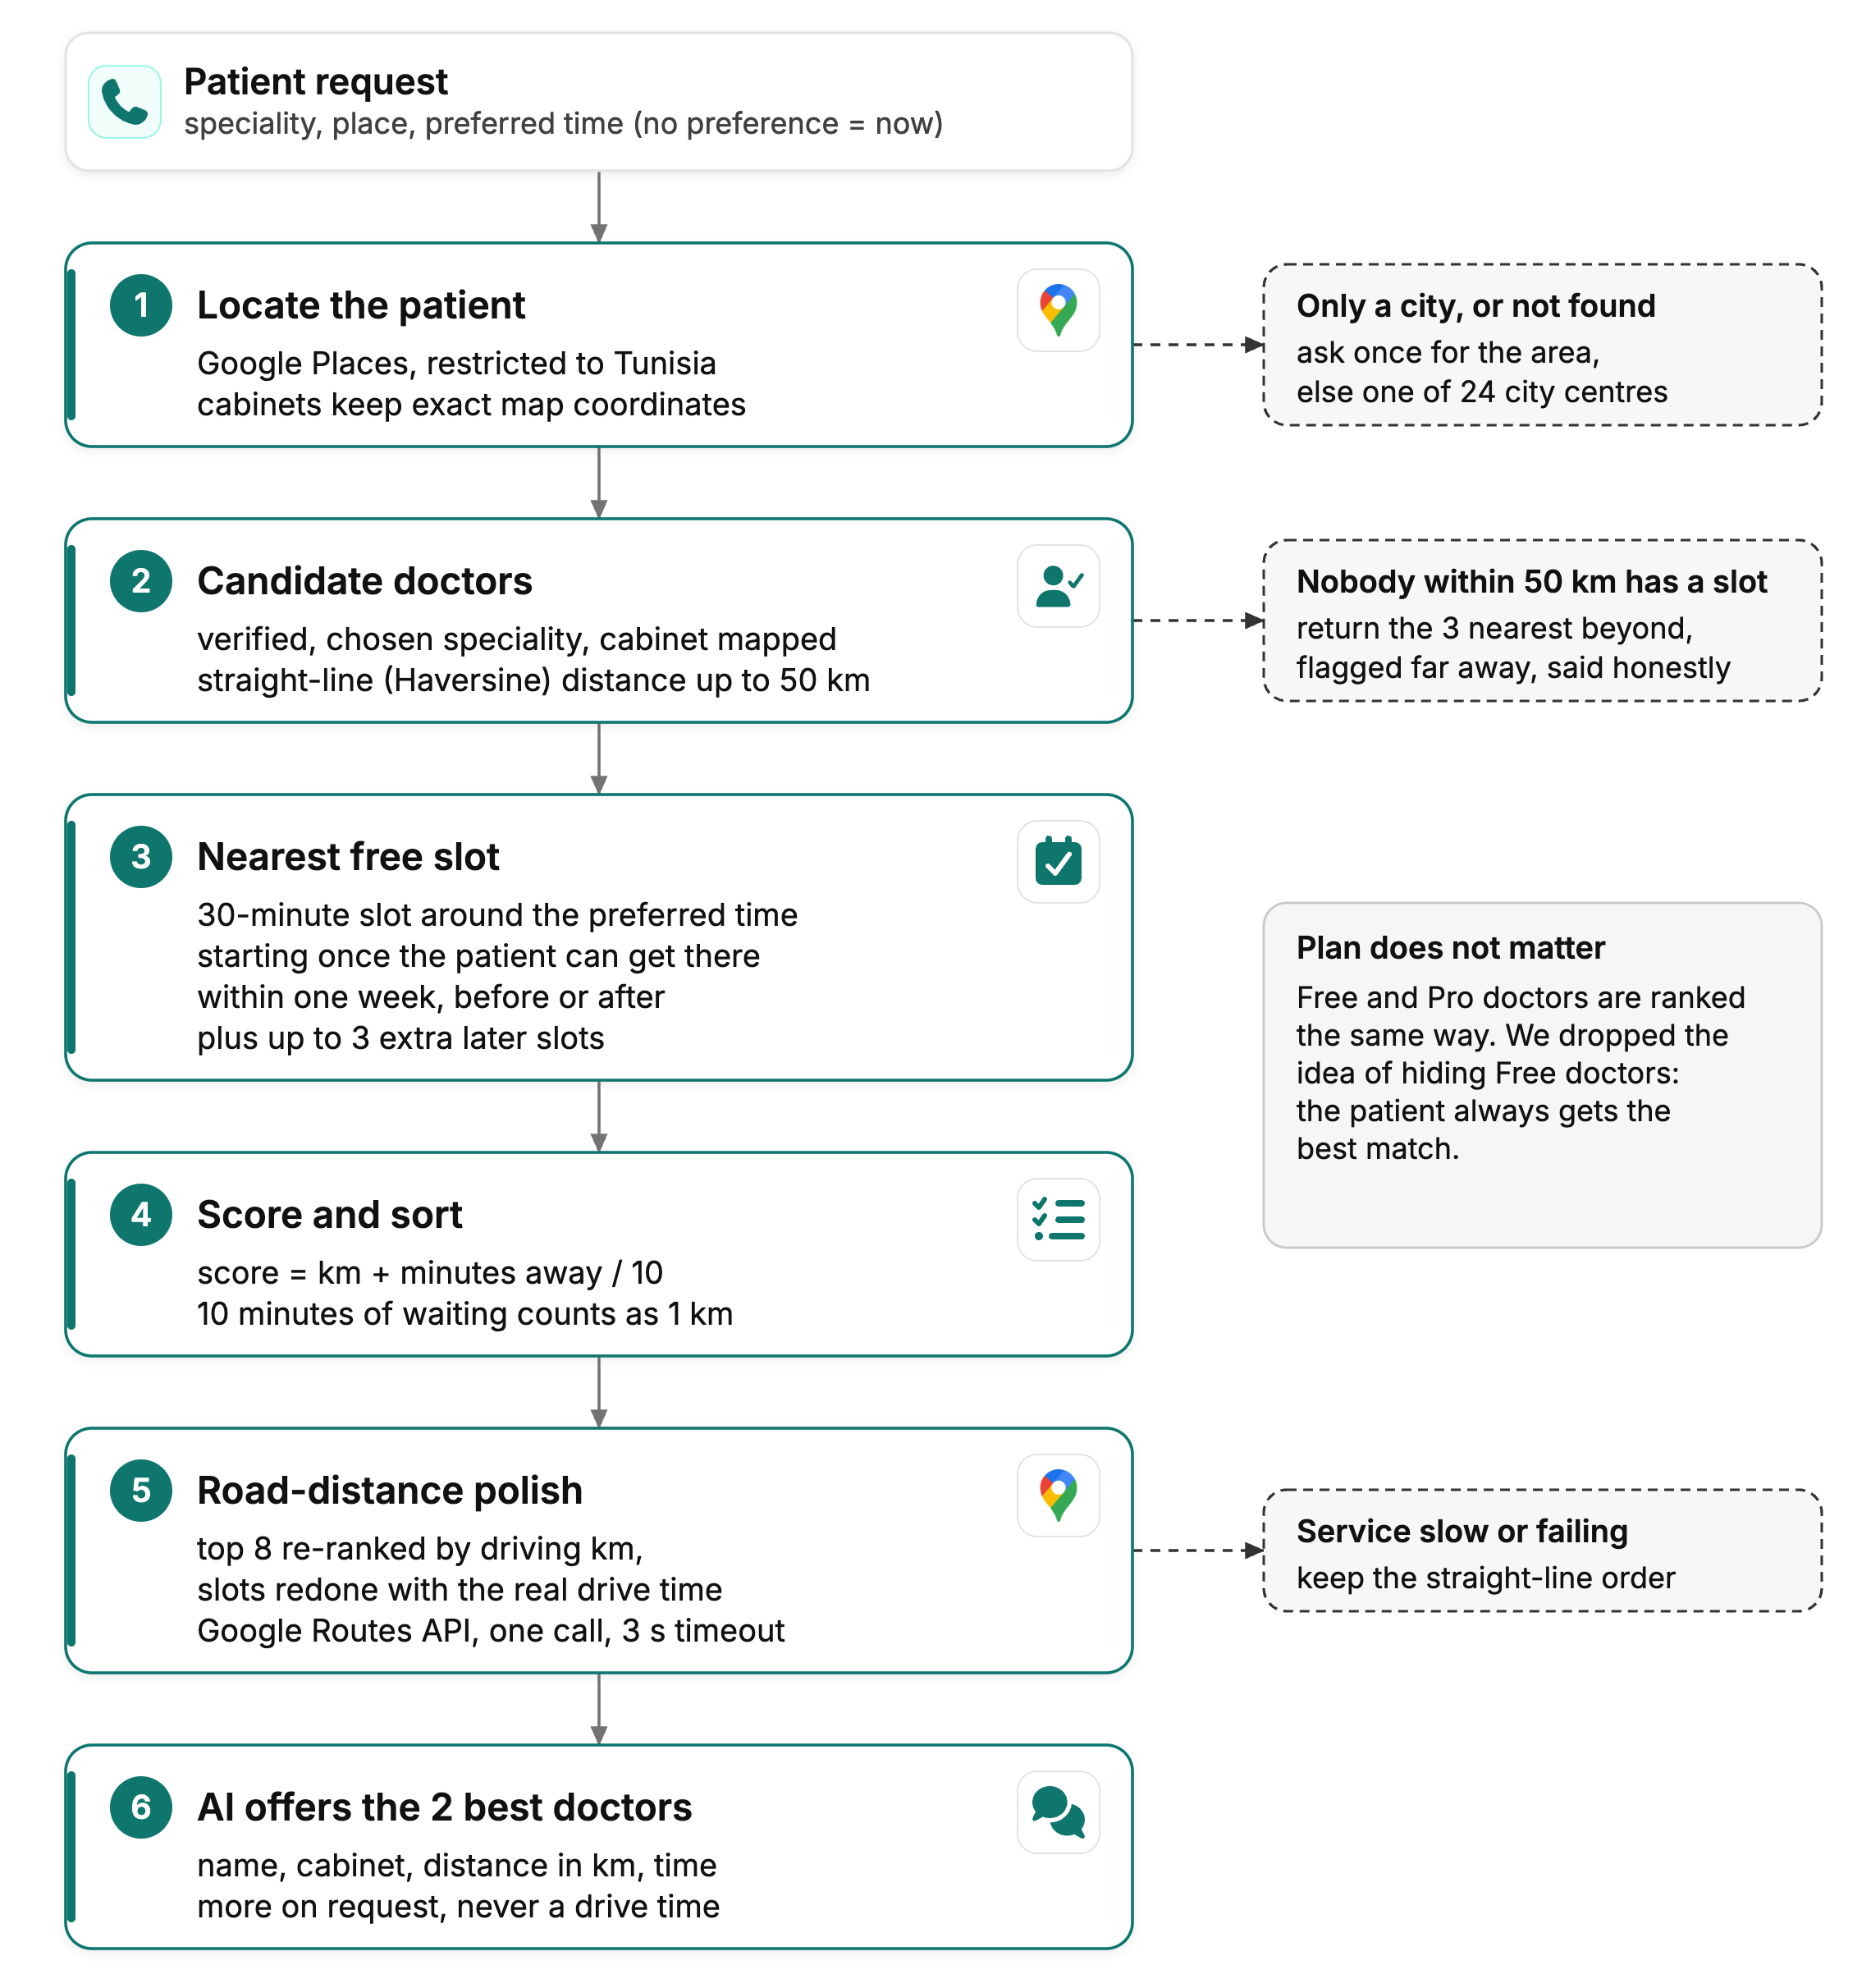
\includegraphics[width=0.85\textwidth,height=0.62\textheight,keepaspectratio]{images/diagrams/bestfit_pipeline.png}
    \caption{The best-fit pipeline, from the patient's request to the 2 or 3 doctors the AI offers}
    \label{fig:bestfit_pipeline}
\end{figure}

\begin{enumerate}
    \item \textbf{Locate the patient.} If this phone line has booked before, the AI first asks whether the patient is in the same area as last time and, if so, reuses that place. Otherwise the place the patient names is looked up with Google Places, restricted to Tunisia. If no precise place is found, the AI falls back to a stored list of 24 Tunisian cities with GPS coordinates. Doctors store the exact coordinates of their cabinet, picked on a map at registration, so the search compares coordinates and not city names.
    \item \textbf{Candidates.} Only verified doctors with the chosen speciality and a mapped cabinet are kept, and doctors that an administrator has excluded from referrals are left out (\secref{subsec:reviews}). Doctors farther than 50~km in a straight line, computed with the Haversine formula, are left out, so a patient in Tunis is not offered a doctor in Sfax. If nobody within 50~km has a free slot, the 3 nearest doctors beyond that limit are returned with a ``far away'' flag, and the AI tells the patient so. Before this fallback, such a search returned nothing.
    \item \textbf{Nearest free slot.} For each doctor, the search finds the free 30-minute slot closest to the preferred time within the next week, before or after it, skipping existing appointments and hours outside the doctor's weekly availability. Up to 3 later slots are kept, so the AI can offer other times without a new search.
    \item \textbf{Score and sort.} Each doctor gets the score below. Lower is better, and 10 minutes of waiting count as much as one kilometre. The time difference is measured against what the patient asked for, not against the current time.
    \item \textbf{Road-distance polish.} The 8 best doctors by straight line are sorted again by driving distance, with one call to the Geoapify Route Matrix and a 3-second timeout. If the service is slow or fails, the straight-line order stays.
    \item \textbf{Answer.} The AI offers the top 2 or 3 doctors with the name, the cabinet address, the distance and the time. It always speaks distance in kilometres, which is how people in Tunisia talk about distance, and never gives a drive time.
\end{enumerate}

\[
\text{score} = \text{distance (km)} + \frac{\lvert \text{slot} - \text{preferred time} \rvert \text{ (minutes)}}{10}
\]

\paragraph{The doctor's plan.} The doctor's plan plays no part in this ranking. When we designed the plans, we considered leaving Free doctors out of the results, so that doctors would have one more reason to subscribe to Pro. We dropped the idea. A patient who calls Riaya should always be offered the doctor who best matches their need, place and time, whatever plan that doctor pays for, and hiding a closer doctor to sell subscriptions would make the service worse for the people it is built for. The plans only limit features on the doctor's side.

\paragraph{Design choices.} A single score lets the search compare a doctor who is close but free later with one who is farther away but free sooner. With 10 minutes of waiting worth one kilometre, a doctor 5~km away at the requested time comes before a doctor next door who is free only one hour later. The 50~km radius keeps the offers to trips that patients would actually make, and the far-away fallback means that a patient in an area with few doctors still gets an answer, with a clear warning about the distance. Road distance comes last and only reorders the 8 best doctors. Our experiment on 78 searches (\secref{subsec:road-distance-experiment}) showed that it changes the best doctor in about one search out of three but never saves more than about 4 minutes of driving. We therefore kept it as a light polish, whose main benefit is that the AI can quote a real road distance.

\paragraph{Prices.} The search does not use prices, and the platform does not show them. We first wanted to, since price matters when choosing a doctor. The price of a first consultation is easy to give, but the real cost depends on what follows, and two doctors with the same consultation price can charge very different amounts for it. Letting doctors enter a price for each service works for services with a fixed price, such as braces. Most patients, though, do not know what they need before a diagnosis, and an AI cannot make that diagnosis over the phone. A partial price could mislead patients, so we left prices out.

\paragraph{Geocoding.} The search is only as good as the patient's position. Callers name neighbourhoods, hospitals, schools and streets, usually in Derja or in French, so we compared several place search services on Tunisian places before choosing Google Places. \secref{subsec:geocoding-evaluation} describes that comparison. Google is not perfect either, and some names exist in several towns, so the AI also gets the list of Tunisian cities and asks the patient to choose when several places match.

\subsection{Urgent Requests and Timeouts}\label{subsec:urgencies}

Some callers are in danger. When a caller describes signs of a life-threatening condition, such as chest pain, trouble breathing, signs of a stroke, heavy bleeding, fainting, a seizure or a serious injury, the AI first tells them to call the SAMU at 190. Riaya books visits and does not replace the emergency services, so the offer of urgent requests to nearby doctors only comes after that advice. For urgent cases that are not life-threatening, the AI asks whether the patient wants the closest available doctors right now. \xref{fig:activity_urgent} in \chapref{chap:management} shows the whole flow.

A patient in an urgent case should not wait 10 minutes for one doctor and then start again. An urgent booking therefore runs the best-fit search with ``now'' as the preferred time and sends up to 3 pending requests at once, all sharing one emergency group id. The first doctor to accept keeps the patient and the other requests of the group are cancelled automatically, so the patient never ends up with several appointments. A doctor who refuses cancels only their own request, since the others can still accept, and for the same reason a refused urgent request triggers no callback. When the patient cancels one urgent request by phone, the whole group is cancelled. If nobody accepts within 10 minutes, a delayed BullMQ job cancels the group and Riaya calls the patient back, as for a normal request. Urgent requests are never limited by a doctor's plan. The delayed jobs and the events between the servers follow the message-based style described by Hohpe and Woolf.

\subsection{Refusals and Callbacks}
\label{subsec:rejection-handling}

We had to decide what happens when a doctor refuses a request or does not answer. Our first idea was to ask the patient for a backup doctor during the call. The call already asks many questions, though, and we wanted to keep it short. So the patient picks one doctor, and if that doctor says no or stays silent, Riaya calls the patient back with new options. After a refusal, Riaya keeps what the patient asked for in Redis for 24 hours, and the AI speaks first in the callback and offers up to 3 other doctors with free slots. If the patient calls Riaya before that, the AI offers these doctors first. After a timeout, the callback only asks the patient to call again. A callback that does not reach the patient is replaced by the same message on WhatsApp from the platform account, and blocked numbers get neither. \xref{fig:bpmn_callback} in \chapref{chap:management} shows the three outcomes of a normal request, and \xref{fig:sequence_callback} shows how the queue, the web app, the voice server and Twilio work together for these callbacks.

\subsection{Patient Reviews and Referral Quality}\label{subsec:reviews}

Two hours after a confirmed visit, a delayed BullMQ job sends the patient a WhatsApp link to the review page (\xref{fig:scr_review}). The job is tied to the appointment. When a doctor moves a confirmed appointment on the calendar, the job is replaced, so the link still arrives two hours after the new end time. When the job runs, it checks again that the appointment is confirmed and that the visit is over.

Each visit can be rated once. A patient who comes often should not get a message after every visit, so no new request goes to a patient who already received one for the same doctor in the last 30 days, whether they answered it or not. A link stops working 30 days after it was sent.

We first built a rating page for doctors and then removed it. Few patients write a comment, a doctor with 30 visits a month collects only a handful of ratings, and a doctor who sees a low score may blame the assistant that booked the patient. The ratings are used by Riaya instead, to decide which doctors the phone assistant keeps offering to callers. Doctors see no rating anywhere.

The Ratings page (\xref{fig:scr_ratings}) shows for each doctor the average rating, the average over the last 90 days, the number of reviews and the share of long waits. Each patient counts once in the average: the ratings of one patient are averaged first, so a patient who comes every week does not set the score alone. Below 5 reviews the values are shown in grey and the doctor is sorted after the doctors with enough reviews. A doctor with an average under 3 over at least 5 reviews is highlighted in red.

The decision stays with the administrator, who opens the doctor's reviews and can stop referrals with a written reason (\xref{fig:scr_rating_detail}). The doctor then disappears from the best-fit search, from urgent requests and from the Best Fit Finder, but keeps the account, the existing appointments and the patients who ask for them by name. We did not lower a doctor's rank automatically from the ratings, because each doctor has too few reviews for such a score to be trusted, and some ratings may judge the booking more than the visit. The excluded doctor sees a banner with the administrator's reason and the support address (\xref{fig:scr_referral_banner}), and no score.

\section{Consultation Recordings}\label{sec:recordings}

A doctor records a consultation in the browser from the Recordings page (\xref{fig:scr_recordings}) and can attach it to a patient. While the recording runs, the browser keeps a copy of the audio in IndexedDB, saved in small pieces, so a closed tab, a refresh or a crash does not lose the consultation. When the doctor stops, the browser uploads the audio straight to Cloudflare R2 with a presigned URL, and the web application saves the recording and processes it in the background.

The audio is transcribed with Microsoft MAI Transcribe 2 through OpenRouter, with speaker separation turned on, so each part of the transcript has a time and a speaker number. The voice model tests ruled this model out for phone calls because it only works on a finished file (\secref{subsec:voice-model-evaluation}), which is exactly what a recording is. The transcriber only numbers the speakers, so a second call, to the chat model (DeepSeek V4 Flash by default), reads the transcript and decides which speaker is the doctor, the patient or a companion. The same call gives the recording a title from what was said, unless the doctor already named it. The doctor can correct the roles if the model got them wrong (\xref{fig:scr_recording}).

On the Pro plan, the chat model then writes a consultation note with five parts: reason for the visit, history, examination, assessment and plan. It writes in French, the usual language of medical records in Tunisia, even when the consultation was in Derja, and keeps drug names and doses as they were said. It only uses what was said and leaves a part empty when it was not discussed, so it never adds a diagnosis or a treatment of its own. The doctor can edit the note or write it again. When the recording is attached to a patient, the note appears in that patient's file, and the AI assistant can read it.

Recording time is counted from the length that the transcriber reports, not from the browser's timer, so a client cannot under-report it. Each recording is charged once, so a retry after a failed transcription is free. When no recording time is left, the recording is still saved, marked as not transcribed, and the doctor can transcribe it later, for example after buying an hour pack.

\section{AI Assistant}\label{sec:assistant}

The assistant is a chat in the doctor's dashboard (\xref{fig:scr_ai_assistant}). It answers medical questions and questions about how to use Riaya, and it works on the practice's own data. Its instructions include a short guide to the dashboard and the plan limits, so it can explain the product as it is. It uses the same chat model as the recordings, through OpenRouter.

The model never reads the database directly. It gets two kinds of tools. The read tools return the schedule between two days, the pending bookings, the patients found by name or CIN, a summary of one patient (appointments, medical files, notes from recordings and unpaid invoices), the free slots of a day, the invoices and the practice statistics. The action tools prepare a change: an invoice, the answer to a pending booking, a note for a medical file, a new appointment or a new time for an existing one. An action tool saves nothing. Its proposal appears as a card that the doctor can edit, then confirm or dismiss, and nothing changes until the doctor confirms. The confirmation calls the same API route as the normal screens, so the usual checks on ownership, overlaps and plan limits apply. The model never invents ids: it gets them from its search tools, and the server checks each one.

A recording can be brought into the chat. The doctor attaches a finished transcript to a question, or opens the assistant from a recording with \textit{Discuss with AI}, and can then ask about the consultation, for example to review the reasoning or draft a summary.

One reply can take up to six model calls, since the model may call a tool, read the result and continue. The reply runs on the server apart from the request: if the doctor closes the page, it still finishes and is saved, and the doctor can stop it at any time. Only the last 20 messages go back to the model with each new question. The use of the assistant is limited by what its replies cost and not by the number of messages (\secref{subsec:usage-limits}), and \secref{sec:security} explains how patient data is kept private.

\section{Evaluations and Tests}\label{sec:evaluations}

Several choices in Riaya depended on how outside services behave with Tunisian places and Tunisian speech, which their documentation does not tell. We therefore tested the options ourselves before settling on them. The comparison of geocoding providers led us to Google Places, the road-distance experiment showed how much the Route Matrix step adds to the best-fit search, and the voice model tests led to Gemini Live. The last subsection explains how the platform as a whole was tested.

\subsection{Geocoding Provider Evaluation}
\label{subsec:geocoding-evaluation}

The first version of the search used Geoapify to find places. Before settling on a provider, we compared several of them on the same Tunisian queries, among them Geoapify, Mapbox and Google Places.

We wrote a list of real places of the kinds patients mention: hospitals, universities, train stations, and the addresses of doctors' cabinets, all written in French, the way most addresses are written in Tunisia. For each place we knew the true position. We sent every query to each provider, restricted to Tunisia, and compared the position it returned with the true one, looking at two things: whether the provider found the place at all, and how far its answer was from the real position.

Google Places was clearly the best. It found many more of the places, including clinics, businesses and smaller institutions that the others did not know, and the positions it returned were more accurate. Geoapify and Mapbox were weaker on both points, so Geoapify was only used for these tests and Google Places became the provider for finding places. The code keeps a switch between the two providers behind one interface, so the rest of the search does not depend on the choice. Google's autocomplete and place details calls share a session token, which counts them as one lookup.

Road distance is a different service. For the polish step of the best-fit search we still use Geoapify's Route Matrix, which returns the driving distances to the 8 candidates in a single call.

\subsection{Road Distance Experiment}
\label{subsec:road-distance-experiment}

Road distance costs a call to an outside service on every search, so we measured whether it changes the result. We ran the search for the 4 specialities with the most doctors, with the patient at the centre of each of the 24 cities, which gave 78 comparisons with no failed call. For each one we took the 8 nearest doctors by straight line and asked for their road distance. \xref{tab:road-distance} shows the results. In one case in Tunis, the nearest doctor was 1.3~km away in a straight line but 5.8~km by road, while another doctor was 2.3~km away both ways; road distance correctly picks the second one. Overall, the best doctor changed in about one search out of three, but the trip saved was small, never more than about 4 minutes. Straight-line distance is therefore a good first filter, and road distance is a light polish whose main benefit is that the AI can quote a real road distance. The test has limits: it used distance only, without appointment times, it placed patients at city centres, it ran on our local data, which may include test doctors, and it only checked the 8 nearest doctors.

\begin{table}[H]
    \centering
    \caption{Effect of road distance on the best doctor (78 searches)}
    \label{tab:road-distance}
    \small
    \begin{tabular}{>{\raggedright\arraybackslash}p{\dimexpr 0.5385\dimexpr\textwidth-4\tabcolsep\relax\relax}>{\raggedright\arraybackslash}p{\dimexpr 0.4615\dimexpr\textwidth-4\tabcolsep\relax\relax}}
        \toprule
        \textbf{Measure} & \textbf{Result} \\
        \midrule
        Best doctor changes (road kilometres) & 24 of 78 (31\%) \\
        Best doctor changes (drive time) & 19 of 78 (24\%) \\
        Time saved when the doctor changes & Median 0.8 min, maximum 4.1 min \\
        Searches saving 5 minutes or more & 0 \\
        Road distance divided by straight distance & Typically 1.01; 1.9 or more for the worst 10\%; 3.27 at worst \\
        \bottomrule
    \end{tabular}
    \\[0.2cm]
\end{table}

\subsection{Voice Model Evaluation and Selection}
\label{subsec:voice-model-evaluation}

The phone call is the reason patients use Riaya, so most of our testing time went into it.

\subsubsection{Two Ways to Build a Phone Call}

In the first approach, called \emph{speech to speech} or realtime, one model listens to the caller and answers with its own voice. It is fast and sounds natural, but the whole conversation depends on one provider. OpenAI Realtime and Gemini Live work this way. The second approach is a \emph{chain of steps}: a speech-to-text model writes down what the caller said, a language model (LLM) writes the answer, and a text-to-speech model reads it out. We could then pick the best model for each step, but every step adds its own wait. We built the chain with LiveKit Agents, which lets us swap the model of each step with a setting. We tested both approaches with the same instructions and the same booking tools.

\subsubsection{Test Method and Its Limits}

We wrote a small program that acts like a phone caller. It plays the same 7 sentences every time, in Tunisian Arabic, in French, and mixed, such as \textit{``\foreignlanguage{arabic}{نحب ناخذ} rendez-vous \foreignlanguage{arabic}{عند} dermatologue''} (``I want to book an appointment with a dermatologist''). It uses the real instructions and booking tools, records what the AI answers, and measures how long each answer takes. We also timed each step of the chain on its own to find where the time went.

To compare engines on full calls, we then built the \texttt{/test-call} page. A tester can call from the browser and choose, for each call, the realtime backend or the model of each step of the chain, plus the model of the caller transcriber. Every option shows our rating, a note, its speed and its price. Only simulated calls read these settings, so real calls always use the server's configuration. The method has a clear limit: the test sentences were spoken by computer voices, not by real patients on real phone lines, and the ratings are our own judgement on a small set of sentences. Prices below come from OpenRouter's model list, checked on 11 October 2026; where we give none, the model runs on another provider.

\subsubsection{The Challenge of Tunisian Arabic}

For English and French, almost every model we tried worked. Tunisian Arabic (Derja) is where they differed, and it was the main problem from the start. Few models understand it. One returned nothing at all for Arabic, and others dropped or misspelled words. Sentences that mix Derja with French words were the hardest: many models wrote the French words in Arabic script, so \textit{dermatologue} came back as an Arabic transliteration that the rest of the system could not match. Few voices speak Derja well either, and several models have no Arabic voice at all. We judged every choice on Tunisian Arabic first, because that is how most patients speak.

\subsubsection{Realtime Models}

\xref{tab:realtime-models} gives our verdicts on the realtime models. OpenAI Realtime was the first one we tested and the smartest of the early tests, but its voice did not have the right accent and it was very expensive. Among the Gemini models, the first versions spoke a good dialect but understood the caller poorly, and the extended-thinking version failed to use the tool results in 8 of 18 tries. \texttt{gemini-3.1-flash-live-preview} was the best of the family. It answered in 1.6 to 4.5 seconds, the longer times when it first had to call a tool.

\begin{table}[H]
    \centering
    \caption{Realtime (speech-to-speech) models tested}
    \label{tab:realtime-models}
    \small
    \begin{tabular}{>{\raggedright\arraybackslash}p{\dimexpr 0.3066\dimexpr\textwidth-6\tabcolsep\relax\relax}>{\raggedright\arraybackslash}p{\dimexpr 0.1387\dimexpr\textwidth-6\tabcolsep\relax\relax}>{\raggedright\arraybackslash}p{\dimexpr 0.5547\dimexpr\textwidth-6\tabcolsep\relax\relax}}
        \toprule
        \textbf{Model} & \textbf{Verdict} & \textbf{What we found} \\
        \midrule
        Gemini Live, \texttt{3.1-flash-live-preview} & Chosen & Tunisian dialect almost perfect, very fast, very good with interruptions, the best reasoning of the Gemini models, understands well. Its own transcript of the caller is very inaccurate. \\
        OpenAI Realtime & Good, not chosen & Fast, good speech recognition, the smartest model of the first tests, very good with interruptions. The voice does not have the right accent, and it is very expensive. \\
        GPT-Live (\texttt{gpt-live-1}) & Bad & Fast, but sounds too artificial, makes mistakes, and the flow is not smooth. Costly, because it runs two models. \\
        \midrule
        \multicolumn{3}{p{14.4cm}}{\textit{Others:} \texttt{gemini-3.8-live} (good dialect and speed, weak understanding), \texttt{gemini-3.8-live} with extended thinking (decent accent, weak understanding, failed to use tool results in 8 of 18 tries), \texttt{gpt-realtime-2.1} (fast, good pronunciation, weak understanding of Arabic and flow), Inworld (about 2.2 s per answer, weak in Arabic, only two Arabic voices).} \\
        \bottomrule
    \end{tabular}
\end{table}

\subsubsection{Speech to Text}

For the chain, the listening step had to handle Derja and keep French words in Latin script. \xref{tab:stt-models} shows the main results. The models that wrote the best text could not stream, so they waited for the end of each sentence before starting. MAI Transcribe 2 gave two different pictures: in the first timed chain it was the best on our sentences, at about 0.5 seconds, but in the later 7-clip run it wrote French words in Arabic script, so we rated it bad for calls. It is still the model that transcribes the doctors' consultation recordings, where it also tells the speakers apart.

\begin{table}[H]
    \centering
    \caption{Main speech-to-text models tested}
    \label{tab:stt-models}
    \small
    \begin{tabular}{>{\raggedright\arraybackslash}p{\dimexpr 0.3066\dimexpr\textwidth-6\tabcolsep\relax\relax}>{\raggedright\arraybackslash}p{\dimexpr 0.1387\dimexpr\textwidth-6\tabcolsep\relax\relax}>{\raggedright\arraybackslash}p{\dimexpr 0.5547\dimexpr\textwidth-6\tabcolsep\relax\relax}}
        \toprule
        \textbf{Model} & \textbf{Verdict} & \textbf{What we found} \\
        \midrule
        Gemini 3 Flash (preview) & Good & Clean French, Derja in Arabic script, French words in Latin script. Slow (about 1.5 s), no streaming. Once wrote a dialogue instead of a transcript. \$0.50 in, \$3.00 out. \\
        \texttt{gemini-3.1-flash-lite} & Pretty good & Fast for a non-streaming model (about 0.8 s), but still too slow for a smooth conversation. Used for the caller transcriber. \$0.25 in, \$1.50 out. \\
        \texttt{gpt-transcribe} & OK & Streams; accepts a list of languages and keywords. Same results as \texttt{gpt-live-transcribe} on the 7 clips. \\
        MAI Transcribe 2 & Bad for calls & Batch only. Turns French words into Arabic script. \\
        Deepgram \texttt{nova-3} & Bad & With an Arabic hint, French and English came back empty; in automatic mode, Derja came back empty. \\
        AssemblyAI Universal & Bad & Not accurate in Arabic, although it keeps French words in Latin script. \\
        \midrule
        \multicolumn{3}{p{14.4cm}}{\textit{Others:} \texttt{gpt-4o-transcribe} and \texttt{gpt-live-transcribe} (bad), \texttt{gemini-3.8-flash} (ok, best on code-switching, waits for each sentence), \texttt{gemini-3.5-flash-lite} (bad, writes Derja in Latin letters), Whisper large v3 turbo, \texttt{gemini-3.5-transcribe}, \texttt{gpt-realtime-whisper}.} \\
        \bottomrule
    \end{tabular}
\end{table}

\subsubsection{Language Model}

The language model of the chain had to follow a long prompt, call the booking tools correctly, and start answering fast. \xref{tab:llm-models} shows what we found. Two numbers come from the timed chain: GPT-5.4 mini started its answer in about 1.2 seconds, and Claude Sonnet, the smartest model we tried, took about 3.6 seconds, three times longer.

\begin{table}[H]
    \centering
    \caption{Main language models tested in the chain}
    \label{tab:llm-models}
    \small
    \begin{tabular}{>{\raggedright\arraybackslash}p{\dimexpr 0.3066\dimexpr\textwidth-6\tabcolsep\relax\relax}>{\raggedright\arraybackslash}p{\dimexpr 0.1387\dimexpr\textwidth-6\tabcolsep\relax\relax}>{\raggedright\arraybackslash}p{\dimexpr 0.5547\dimexpr\textwidth-6\tabcolsep\relax\relax}}
        \toprule
        \textbf{Model} & \textbf{Verdict} & \textbf{What we found} \\
        \midrule
        \texttt{gemini-2.5-flash} & Current & Follows the context well, speed acceptable. The model set in the LiveKit chain today. \$0.30 in, \$2.50 out. \\
        \texttt{gemini-2.5-flash-lite} & Bad & Cheap (\$0.10 in, \$0.40 out) but made too many mistakes in the conversation. \\
        \texttt{gemini-3.8-flash} & Bad & Too slow to answer. \$0.75 in, \$3.75 out. \\
        GPT-5.4 mini & Not kept & The first LLM of the chain; fast to start (about 1.2 s) but less smart than Claude. \$0.75 in, \$4.50 out. \\
        Claude Sonnet and Haiku & Not kept & Sonnet was the smartest but about 3 times slower to start (3.6 s). Haiku was considered and not tried in a call. \\
        \midrule
        \multicolumn{3}{p{14.4cm}}{\textit{Others:} \texttt{gemini-3.1-flash-lite} (set briefly, then replaced), \texttt{gpt-4.1-mini} (considered, not set).} \\
        \bottomrule
    \end{tabular}
\end{table}

\subsubsection{Text to Speech}

For the voice, the problem was the opposite of listening: the voices that spoke real Tunisian Arabic were the slowest, and the fast ones had no Tunisian accent. \xref{tab:tts-models} shows the main results.

\begin{table}[H]
    \centering
    \caption{Main text-to-speech models tested}
    \label{tab:tts-models}
    \small
    \begin{tabular}{>{\raggedright\arraybackslash}p{\dimexpr 0.3066\dimexpr\textwidth-6\tabcolsep\relax\relax}>{\raggedright\arraybackslash}p{\dimexpr 0.1387\dimexpr\textwidth-6\tabcolsep\relax\relax}>{\raggedright\arraybackslash}p{\dimexpr 0.5547\dimexpr\textwidth-6\tabcolsep\relax\relax}}
        \toprule
        \textbf{Model} & \textbf{Verdict} & \textbf{What we found} \\
        \midrule
        Gemini TTS, voice Charon & Best voice, too slow & The flash model has the best voice we heard, with an almost perfect Tunisian dialect, but takes 4 to 5 s. The flash-lite model is very good and takes about 2 s; streamed from Google's API, the first audio came after 0.6 to 1.2 s. \\
        xAI \texttt{tts-1} & Not kept & Very fast (about 0.25 s) and pronounces Arabic, but without a Tunisian accent. \$15 per million characters. \\
        Inworld, voice Omar & Maybe & Fast, used before the switch, but no Tunisian accent and only two Arabic voices. \\
        ElevenLabs \texttt{eleven-v4} & Bad & About 1.5 s, acceptable accent, but very expensive (about \$40 per million characters). \\
        MAI Voice & Bad & Fast (about 0.5 s), but none of its 97 voices is Arabic. \\
        \midrule
        \multicolumn{3}{p{14.4cm}}{\textit{Others:} \texttt{gemini-3.1-flash-tts-preview} (slow, accent not Tunisian), \texttt{gpt-4o-mini-tts} (about 3 s, not streamed), Kokoro, Fish Audio and Deepgram Aura-2 (no Arabic voice).} \\
        \bottomrule
    \end{tabular}
\end{table}

\subsubsection{Lessons Learned}

The best models were often the slowest: the best listening model and the best voice were both slow. In a chain, the delays add up, because the caller waits for every step in turn. \xref{tab:voice-model-comparison} shows the step timings of the chains we measured. The fastest chain we built waited about 6.8 seconds before answering, and with Gemini for both listening and the voice it took more than 10 seconds, far too long for a phone conversation.

\begin{table}[H]
    \centering
    \caption{Speed of each step in the chains we timed}
    \label{tab:voice-model-comparison}
    \small
    \begin{tabular}{>{\raggedright\arraybackslash}p{\dimexpr 0.1571\dimexpr\textwidth-8\tabcolsep\relax\relax}>{\raggedright\arraybackslash}p{\dimexpr 0.2143\dimexpr\textwidth-8\tabcolsep\relax\relax}>{\raggedright\arraybackslash}p{\dimexpr 0.3143\dimexpr\textwidth-8\tabcolsep\relax\relax}>{\raggedright\arraybackslash}p{\dimexpr 0.3143\dimexpr\textwidth-8\tabcolsep\relax\relax}}
        \toprule
        \textbf{Step} & \textbf{Model} & \textbf{What we found} & \textbf{Problem} \\
        \midrule
        Listening & Microsoft MAI & Best on our sentences, about 0.5 s & A preview product with one provider \\
        Listening & Gemini & Excellent text & 2 to 3 s per sentence \\
        Listening & Inworld & Fast & Not good in Arabic, worst on mixed sentences \\
        Thinking & GPT-5.4 mini & Fast, about 1.2 s to start & Less smart than Claude \\
        Thinking & Claude Sonnet & The smartest & 3 times slower to start (3.6 s) \\
        Voice & Gemini & The most natural & 2 to 3 s before it talks \\
        Voice & Inworld & Fast & Only 2 Arabic voices, not perfect \\
        \bottomrule
    \end{tabular}
\end{table}

The tests also found a real bug. The AI saved the caller's name or language on almost every turn, and each save cost about one extra second. In the LiveKit chain we moved this to a background job that reads each caller sentence with a small model and saves the profile without making the caller wait.

\subsubsection{Final Choice}

We chose Gemini Live with the \texttt{gemini-3.1-flash-live-preview} model and the Puck voice. Of all the models we tried, it had the most natural Tunisian dialect, it answered very fast, it handled interruptions very well, and it understood and reasoned best among the Gemini models. OpenAI Realtime was smarter in the first tests, but its accent was wrong for Tunisian callers and it cost much more. GPT-Live sounded too artificial and was also costly, and every chain we built was too slow for a phone call.

Gemini Live's one weakness is its transcript of the caller, which comes from a separate speech-to-text step inside the Live API that we cannot tune. The separate caller transcriber described in \secref{subsec:latency} fixes it for the admin live view and the stored call events. We kept the other realtime backends and the LiveKit chain in the code on purpose, so that new models can be compared again on the test-call page with the same calls.

\subsection{How the Platform Was Tested}

We tested every feature of Riaya, both manually and with AI tools that test every corner of the application. They covered the sign-up and verification steps, the doctor and secretary dashboards, the plans and payments, and the administrator back-office.

Most of the effort went into the phone call, since it is the heart of the product. We first made sure that Twilio worked correctly, with calls to the real number that checked that the phone line reached the assistant on the team's server. Only then did we add the test-call page, to save Twilio's balance: every real call costs money, and a simulated call from the browser costs nothing on Twilio. The page lets us place simulated calls, switch models for each call, and watch the transcript and the tool calls live. The voice server can also send a refusal or timeout callback to an open test-call page instead of placing a real call, so these flows could be tested without Twilio too. We spent a very long time on this page: we made a large number of test calls, compared many models and both approaches described in \secref{subsec:voice-model-evaluation}, and improved the instructions and the booking tools after each round until the assistant handled the calls well.

The comparison of geocoding providers (\secref{subsec:geocoding-evaluation}) and the 78 road-distance comparisons (\secref{subsec:road-distance-experiment}) gave us data for the place search. The admin Best Fit Finder, which runs the same search on a map and a calendar, helped us check the ranking by eye.

The code itself has no automated test suite yet, such as unit tests or end-to-end tests that run on every change. Adding one, starting with the best-fit search, the plan limits and the booking flow, is part of the future work.

\section{Security, Confidentiality, and Access Management}\label{sec:security}

Riaya stores sensitive data: the identity documents that doctors send with their application, patients' medical files, consultation recordings with their transcripts, and recordings of phone calls. This section explains who can reach which data, how the two servers trust each other, and what we did to keep the AI parts and the WhatsApp messages private. It also names the gaps that are still open.

\subsection{Authentication and Authorization}

Accounts are handled by Better Auth with an email and a password. The password needs at least 8 characters, with letters and numbers. At sign-up, Riaya emails a 6-digit code through Nodemailer. The code is valid for 10 minutes and accepts 5 attempts, and a new code can be requested after a 60-second cooldown. These limits follow the usual advice on one-time codes, which is to keep them short-lived and to limit guessing. Until the code is verified, no user row exists. The pending sign-up sits in Better Auth's \texttt{verification} table, with a hash of the code and the password encrypted with AES-256-GCM, and the account is created only when the right code arrives. An address that nobody controls therefore never becomes an account.

An account alone does not make someone a doctor on Riaya. After sign-up the doctor can open only the Profile page, where they fill in an application: CIN pictures (front and back), speciality, Medical Council number and certificate, cabinet name, tax number, and the exact position of the cabinet on a map. An administrator reviews it and approves, rejects with reasons, or bans. Every other dashboard page redirects to Profile until the doctor is verified, so an unverified account cannot receive bookings or see patients.

Authorization is checked on the server for every request. Each API route starts with one of a few helpers: \texttt{requireSession} for any signed-in user, \texttt{requireDoctorProfile} for a verified doctor, \texttt{requirePractice} for routes that a doctor's secretary may also use, \texttt{requireAdmin} for the back office, and \texttt{requireInternal} for calls from the voice server. Hiding a menu item in the interface is never the only protection. Administrators are users whose access level is set in the database; nobody can become one through the sign-up page.

Secretaries are a Pro feature. The doctor invites them by email from the Team page. The link \texttt{/join/<token>} expires after 7 days, can be resent or cancelled, and the database stores only a SHA-256 hash of the token, so a copy of the database does not contain working invitation links. The secretary must sign in with the invited email address. Their access covers the appointments, patients, invoices and availability of that one doctor, without medical files, recordings, the AI assistant or billing. If the doctor drops back to Free or loses verification, the secretary's access is paused, not deleted, and it comes back when Pro is renewed. This follows the principle of least privilege. \xref{tab:auth_matrix} sums up the roles.

\begin{table}[H]
    \centering
    \caption{Authentication and authorization by role}
    \label{tab:auth_matrix}
    \small
    \begin{tabular}{>{\raggedright\arraybackslash}p{\dimexpr 0.1752\dimexpr\textwidth-8\tabcolsep\relax\relax}>{\raggedright\arraybackslash}p{\dimexpr 0.2482\dimexpr\textwidth-8\tabcolsep\relax\relax}>{\raggedright\arraybackslash}p{\dimexpr 0.2847\dimexpr\textwidth-8\tabcolsep\relax\relax}>{\raggedright\arraybackslash}p{\dimexpr 0.2920\dimexpr\textwidth-8\tabcolsep\relax\relax}}
        \toprule
        \textbf{Role} & \textbf{Authentication} & \textbf{Access} & \textbf{Restrictions} \\
        \midrule
        Patient & None; the phone number given by Twilio identifies the line & Phone calls and WhatsApp; a one-time link to rate a doctor & No account and no website; can cancel only pending requests \\
        Doctor & Email and password, email code at sign-up, then admin verification & Full dashboard of their own practice & Profile page only until verified; Pro features need an active Pro plan \\
        Secretary & Email and password, by invitation (link valid 7 days, hashed token) & Appointments, patients, invoices and availability of one doctor & No medical files, recordings, AI assistant, WhatsApp setup or billing; paused when the doctor leaves Pro \\
        Administrator & Email and password; access level set in the database & Back office: applications, live calls and recordings, reports, blocked numbers, users, specialities & Cannot be obtained through sign-up \\
        \bottomrule
    \end{tabular}
\end{table}

\subsection{Protection of Medical Data}

Files are stored in Cloudflare R2. To upload a document, the browser first asks the web app for a presigned URL. This route requires a signed-in user, and the URL it returns is valid for 10 minutes and allows an upload only to a key made of a fixed folder name and a random UUID. The browser then sends the file straight to R2, so medical documents and recordings never pass through our web server, and only the file's link is saved on the record. When a doctor opens a patient, a medical file or a recording, the API first checks on the server that the record belongs to that doctor's practice. Secretaries never receive medical files or recordings, and the AI assistant goes through the same ownership checks for every id it uses.

One weakness remains. The link stored on each record is a public CDN address. The random file names make the links impossible to guess in practice, but anyone who has a link can open the file without signing in, and a link that is forwarded by mistake keeps working. A cleaner design is a private bucket where the API hands out a short-lived signed download link after the same ownership check. We kept this for the future work because it touches every screen that shows a file.

Health data is a sensitive category under the Tunisian law on personal data, and the GDPR is a useful reference for its principles of data minimization and purpose limitation. Riaya keeps little data about patients: no account, no password, and only what the call needs (name, date of birth, gender, address, preferred language), plus the place each phone booking was searched from.

\subsection{Confidentiality of WhatsApp Conversations}

Each doctor links their own WhatsApp account by scanning a QR code on the WhatsApp page. The voice server then sends messages through Baileys from the doctor's own number. Patients see a message from their doctor, and their replies reach the doctor's phone without going through Riaya. Invoices that a secretary sends still leave from the doctor's number. Only system messages, such as the notice that a request expired, come from the platform's own WhatsApp account.

The database has no table for message content. It keeps a monthly counter of the sends a doctor started, for the Free plan limit, and a flag on a medical file once it has been sent. Riaya therefore holds no copy of what doctors and patients write to each other. Baileys works by linking the server as a WhatsApp Web device, so the session keys of each doctor's account live on the voice server. Anyone who controlled that server could send messages as the doctor.

\subsection{Server-to-Server Security}

The voice server calls the web app's internal API to search slots, book, cancel and update a caller's profile. These routes, and the call and person routes the voice server uses, require a shared secret in the \texttt{x-internal-secret} header. The caller's phone number always comes from Twilio and never from the AI, so the model cannot book or cancel for another line, even if a caller tries to make it. The Twilio recording webhook on the web app has to be public, so it checks Twilio's \texttt{X-Twilio-Signature} header (an HMAC-SHA1 of the request) before it accepts a recording. On the voice side, the WebSocket that receives events from the LiveKit agent also requires the shared secret.

Some entry points of the voice server are not protected yet. The \texttt{/incoming-call} webhook does not verify Twilio's signature, and the route the web app uses to send WhatsApp messages, as well as the WebSockets that stream live calls and the WhatsApp QR code, do not check the shared secret or a session. They rely on the voice server's address not being known. Adding the same checks there is one of the first items of the future work.

\subsection{Privacy of the AI Assistant}

The doctor's AI assistant reads patient data, so every chat request it sends to OpenRouter carries two routing options, \texttt{zdr: true} and \texttt{data\_collection: deny}. With them, OpenRouter only uses providers that neither keep nor train on the request. The same options apply to the other chat calls of the web app: recording titles, speaker roles and consultation notes. The two transcription calls, for consultation recordings and for the caller's words on the phone, do not send these options yet, and we plan to add them.

The assistant also cannot change data on its own: every change it prepares waits for the doctor's confirmation and goes through the normal API checks (\secref{sec:assistant}).

\subsection{Abuse Prevention: Reports and Blocked Numbers}

A public phone number attracts abuse. The phone AI gives one calm warning for mockery or insults and calls the \texttt{report\_abuse} tool right away for threats or sexual talk. The prompt tells it never to report confusion, frustration, elderly callers, bad lines, children, jokes, or questions such as ``are you a robot''. When it is not sure, it does not report. It never tells the caller that the call is reported. A report holds a category and a summary written by the AI, and the review page shows it next to the call recording and transcript. Administrators review reports in a queue, and can dismiss one or block the number for 7 days, 30 days or permanently.

Before any AI session starts, the voice server asks the web app whether the caller is blocked. A blocked caller gets a busy signal from Twilio, the attempt is counted, and no recording, callback or WhatsApp message follows. The check has a timeout of about 1.5 seconds and fails open: if the web app is slow or down, the call goes through. We preferred letting an abuser through during an outage to turning away a real patient.
.
% It holds three sections: security and access management, the technical
% challenges with the solutions we adopted, and the evaluations and tests.

\section{Phone Booking}\label{sec:booking}

Phone booking is the main feature of Riaya. This section follows it in the order a patient meets it: the call itself, the search for a doctor, urgent requests, what happens when a doctor refuses or does not answer, and the review after the visit. Each part explains how it works and why we built it that way. The tests behind several of these choices are in \secref{sec:evaluations}.

\subsection{The Call: Latency and Silence Handling}\label{subsec:latency}

During a call, the voice server bridges three WebSocket connections: Twilio's audio stream (G.711 $\mu$-law at 8~kHz), the realtime AI model, and the admin dashboard that shows the live transcript. Every extra millisecond between the caller's last word and the AI's first word makes the call feel less natural. Telephone guidelines aim for a one-way delay of about 150~ms; an AI that has to understand and answer takes far longer, so each step we could remove mattered. The choice of a speech-to-speech model was the biggest gain (\secref{subsec:voice-model-evaluation}). Smaller ones came from the call set-up: the server creates the call row and loads the caller's profile in parallel and caches both, and the check for blocked numbers stops waiting after about 1.5 seconds.

Phone audio is noisy. Before it reaches the model, the caller's audio goes through a high-pass filter that cuts rumble and hum below 250~Hz and a noise gate that follows the background noise level and silences the gaps between words.

Gemini Live understands callers well, but its own transcript of what they said was very inaccurate in our tests, and it cannot be tuned. Since administrators read that transcript in Live Calls and in abuse reports, we added a separate caller transcriber. It splits the caller's audio into sentences with a simple energy check and sends each sentence to \texttt{gemini-3.1-flash-lite} through OpenRouter, which returns it in about 0.8 seconds. It runs beside the conversation, so it does not delay the AI's answers, and it can be turned off with one setting.

Silence was the other problem. Some callers put the phone down without hanging up, and an open call costs money every minute. A shared watchdog, used by the Twilio path and by the LiveKit agent, waits 12 seconds once the assistant is quiet, asks once whether the caller is still there, and says goodbye and hangs up if the caller stays silent for 10 more seconds. Any call ends politely after 15 minutes. Silent calls are logged as a system event and are not treated as abuse.

\subsection{The Best-Fit Search}\label{subsec:bestfit}

While the patient waits on the line, the platform has to turn ``a dermatologist near Ariana tomorrow morning'' into two or three concrete offers. \xref{fig:bestfit_pipeline} shows the six steps of the search.

\begin{figure}[H]
    \centering
    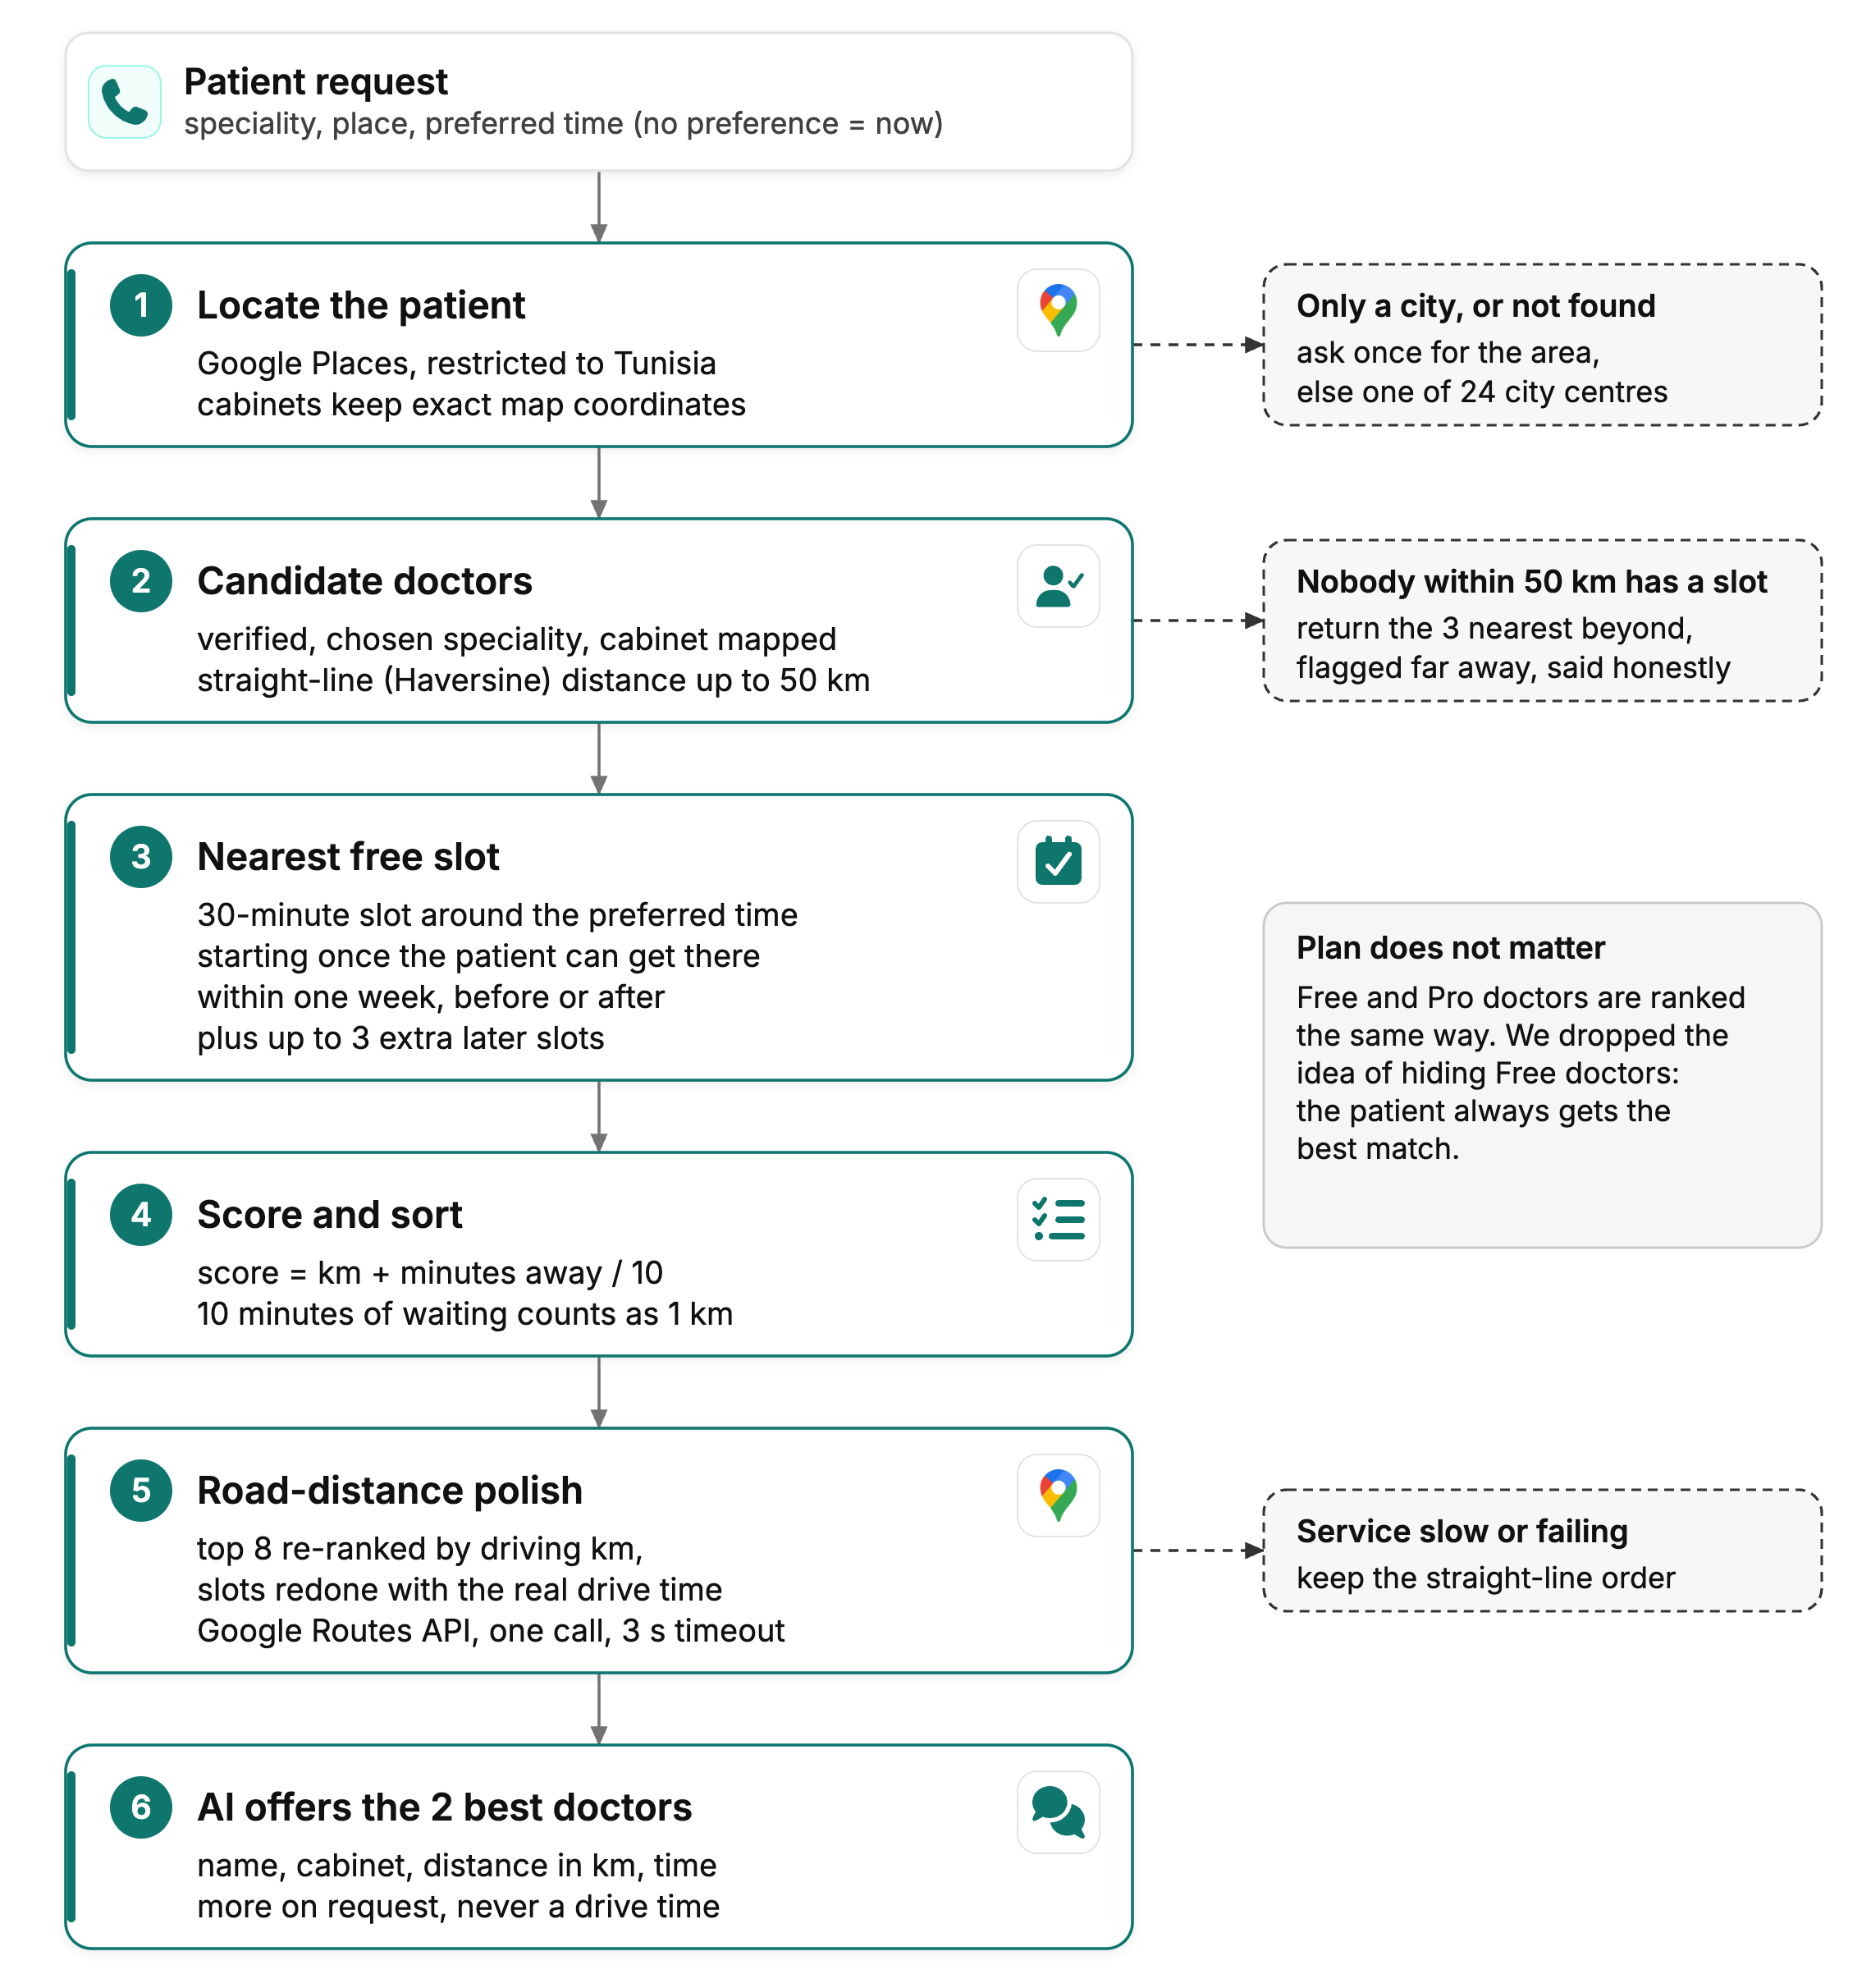
\includegraphics[width=0.85\textwidth,height=0.62\textheight,keepaspectratio]{images/diagrams/bestfit_pipeline.png}
    \caption{The best-fit pipeline, from the patient's request to the 2 or 3 doctors the AI offers}
    \label{fig:bestfit_pipeline}
\end{figure}

\begin{enumerate}
    \item \textbf{Locate the patient.} If this phone line has booked before, the AI first asks whether the patient is in the same area as last time and, if so, reuses that place. Otherwise the place the patient names is looked up with Google Places, restricted to Tunisia. If no precise place is found, the AI falls back to a stored list of 24 Tunisian cities with GPS coordinates. Doctors store the exact coordinates of their cabinet, picked on a map at registration, so the search compares coordinates and not city names.
    \item \textbf{Candidates.} Only verified doctors with the chosen speciality and a mapped cabinet are kept, and doctors that an administrator has excluded from referrals are left out (\secref{subsec:reviews}). Doctors farther than 50~km in a straight line, computed with the Haversine formula, are left out, so a patient in Tunis is not offered a doctor in Sfax. If nobody within 50~km has a free slot, the 3 nearest doctors beyond that limit are returned with a ``far away'' flag, and the AI tells the patient so. Before this fallback, such a search returned nothing.
    \item \textbf{Nearest free slot.} For each doctor, the search finds the free 30-minute slot closest to the preferred time within the next week, before or after it, skipping existing appointments and hours outside the doctor's weekly availability. Up to 3 later slots are kept, so the AI can offer other times without a new search.
    \item \textbf{Score and sort.} Each doctor gets the score below. Lower is better, and 10 minutes of waiting count as much as one kilometre. The time difference is measured against what the patient asked for, not against the current time.
    \item \textbf{Road-distance polish.} The 8 best doctors by straight line are sorted again by driving distance, with one call to the Geoapify Route Matrix and a 3-second timeout. If the service is slow or fails, the straight-line order stays.
    \item \textbf{Answer.} The AI offers the top 2 or 3 doctors with the name, the cabinet address, the distance and the time. It always speaks distance in kilometres, which is how people in Tunisia talk about distance, and never gives a drive time.
\end{enumerate}

\[
\text{score} = \text{distance (km)} + \frac{\lvert \text{slot} - \text{preferred time} \rvert \text{ (minutes)}}{10}
\]

\paragraph{The doctor's plan.} The doctor's plan plays no part in this ranking. When we designed the plans, we considered leaving Free doctors out of the results, so that doctors would have one more reason to subscribe to Pro. We dropped the idea. A patient who calls Riaya should always be offered the doctor who best matches their need, place and time, whatever plan that doctor pays for, and hiding a closer doctor to sell subscriptions would make the service worse for the people it is built for. The plans only limit features on the doctor's side.

\paragraph{Design choices.} A single score lets the search compare a doctor who is close but free later with one who is farther away but free sooner. With 10 minutes of waiting worth one kilometre, a doctor 5~km away at the requested time comes before a doctor next door who is free only one hour later. The 50~km radius keeps the offers to trips that patients would actually make, and the far-away fallback means that a patient in an area with few doctors still gets an answer, with a clear warning about the distance. Road distance comes last and only reorders the 8 best doctors. Our experiment on 78 searches (\secref{subsec:road-distance-experiment}) showed that it changes the best doctor in about one search out of three but never saves more than about 4 minutes of driving. We therefore kept it as a light polish, whose main benefit is that the AI can quote a real road distance.

\paragraph{Prices.} The search does not use prices, and the platform does not show them. We first wanted to, since price matters when choosing a doctor. The price of a first consultation is easy to give, but the real cost depends on what follows, and two doctors with the same consultation price can charge very different amounts for it. Letting doctors enter a price for each service works for services with a fixed price, such as braces. Most patients, though, do not know what they need before a diagnosis, and an AI cannot make that diagnosis over the phone. A partial price could mislead patients, so we left prices out.

\paragraph{Geocoding.} The search is only as good as the patient's position. Callers name neighbourhoods, hospitals, schools and streets, usually in Derja or in French, so we compared several place search services on Tunisian places before choosing Google Places. \secref{subsec:geocoding-evaluation} describes that comparison. Google is not perfect either, and some names exist in several towns, so the AI also gets the list of Tunisian cities and asks the patient to choose when several places match.

\subsection{Urgent Requests and Timeouts}\label{subsec:urgencies}

Some callers are in danger. When a caller describes signs of a life-threatening condition, such as chest pain, trouble breathing, signs of a stroke, heavy bleeding, fainting, a seizure or a serious injury, the AI first tells them to call the SAMU at 190. Riaya books visits and does not replace the emergency services, so the offer of urgent requests to nearby doctors only comes after that advice. For urgent cases that are not life-threatening, the AI asks whether the patient wants the closest available doctors right now. \xref{fig:activity_urgent} in \chapref{chap:management} shows the whole flow.

A patient in an urgent case should not wait 10 minutes for one doctor and then start again. An urgent booking therefore runs the best-fit search with ``now'' as the preferred time and sends up to 3 pending requests at once, all sharing one emergency group id. The first doctor to accept keeps the patient and the other requests of the group are cancelled automatically, so the patient never ends up with several appointments. A doctor who refuses cancels only their own request, since the others can still accept, and for the same reason a refused urgent request triggers no callback. When the patient cancels one urgent request by phone, the whole group is cancelled. If nobody accepts within 10 minutes, a delayed BullMQ job cancels the group and Riaya calls the patient back, as for a normal request. Urgent requests are never limited by a doctor's plan. The delayed jobs and the events between the servers follow the message-based style described by Hohpe and Woolf.

\subsection{Refusals and Callbacks}
\label{subsec:rejection-handling}

We had to decide what happens when a doctor refuses a request or does not answer. Our first idea was to ask the patient for a backup doctor during the call. The call already asks many questions, though, and we wanted to keep it short. So the patient picks one doctor, and if that doctor says no or stays silent, Riaya calls the patient back with new options. After a refusal, Riaya keeps what the patient asked for in Redis for 24 hours, and the AI speaks first in the callback and offers up to 3 other doctors with free slots. If the patient calls Riaya before that, the AI offers these doctors first. After a timeout, the callback only asks the patient to call again. A callback that does not reach the patient is replaced by the same message on WhatsApp from the platform account, and blocked numbers get neither. \xref{fig:bpmn_callback} in \chapref{chap:management} shows the three outcomes of a normal request, and \xref{fig:sequence_callback} shows how the queue, the web app, the voice server and Twilio work together for these callbacks.

\subsection{Patient Reviews and Referral Quality}\label{subsec:reviews}

Two hours after a confirmed visit, a delayed BullMQ job sends the patient a WhatsApp link to the review page (\xref{fig:scr_review}). The job is tied to the appointment. When a doctor moves a confirmed appointment on the calendar, the job is replaced, so the link still arrives two hours after the new end time. When the job runs, it checks again that the appointment is confirmed and that the visit is over.

Each visit can be rated once. A patient who comes often should not get a message after every visit, so no new request goes to a patient who already received one for the same doctor in the last 30 days, whether they answered it or not. A link stops working 30 days after it was sent.

We first built a rating page for doctors and then removed it. Few patients write a comment, a doctor with 30 visits a month collects only a handful of ratings, and a doctor who sees a low score may blame the assistant that booked the patient. The ratings are used by Riaya instead, to decide which doctors the phone assistant keeps offering to callers. Doctors see no rating anywhere.

The Ratings page (\xref{fig:scr_ratings}) shows for each doctor the average rating, the average over the last 90 days, the number of reviews and the share of long waits. Each patient counts once in the average: the ratings of one patient are averaged first, so a patient who comes every week does not set the score alone. Below 5 reviews the values are shown in grey and the doctor is sorted after the doctors with enough reviews. A doctor with an average under 3 over at least 5 reviews is highlighted in red.

The decision stays with the administrator, who opens the doctor's reviews and can stop referrals with a written reason (\xref{fig:scr_rating_detail}). The doctor then disappears from the best-fit search, from urgent requests and from the Best Fit Finder, but keeps the account, the existing appointments and the patients who ask for them by name. We did not lower a doctor's rank automatically from the ratings, because each doctor has too few reviews for such a score to be trusted, and some ratings may judge the booking more than the visit. The excluded doctor sees a banner with the administrator's reason and the support address (\xref{fig:scr_referral_banner}), and no score.

\section{Consultation Recordings}\label{sec:recordings}

A doctor records a consultation in the browser from the Recordings page (\xref{fig:scr_recordings}) and can attach it to a patient. While the recording runs, the browser keeps a copy of the audio in IndexedDB, saved in small pieces, so a closed tab, a refresh or a crash does not lose the consultation. When the doctor stops, the browser uploads the audio straight to Cloudflare R2 with a presigned URL, and the web application saves the recording and processes it in the background.

The audio is transcribed with Microsoft MAI Transcribe 2 through OpenRouter, with speaker separation turned on, so each part of the transcript has a time and a speaker number. The voice model tests ruled this model out for phone calls because it only works on a finished file (\secref{subsec:voice-model-evaluation}), which is exactly what a recording is. The transcriber only numbers the speakers, so a second call, to the chat model (DeepSeek V4 Flash by default), reads the transcript and decides which speaker is the doctor, the patient or a companion. The same call gives the recording a title from what was said, unless the doctor already named it. The doctor can correct the roles if the model got them wrong (\xref{fig:scr_recording}).

On the Pro plan, the chat model then writes a consultation note with five parts: reason for the visit, history, examination, assessment and plan. It writes in French, the usual language of medical records in Tunisia, even when the consultation was in Derja, and keeps drug names and doses as they were said. It only uses what was said and leaves a part empty when it was not discussed, so it never adds a diagnosis or a treatment of its own. The doctor can edit the note or write it again. When the recording is attached to a patient, the note appears in that patient's file, and the AI assistant can read it.

Recording time is counted from the length that the transcriber reports, not from the browser's timer, so a client cannot under-report it. Each recording is charged once, so a retry after a failed transcription is free. When no recording time is left, the recording is still saved, marked as not transcribed, and the doctor can transcribe it later, for example after buying an hour pack.

\section{AI Assistant}\label{sec:assistant}

The assistant is a chat in the doctor's dashboard (\xref{fig:scr_ai_assistant}). It answers medical questions and questions about how to use Riaya, and it works on the practice's own data. Its instructions include a short guide to the dashboard and the plan limits, so it can explain the product as it is. It uses the same chat model as the recordings, through OpenRouter.

The model never reads the database directly. It gets two kinds of tools. The read tools return the schedule between two days, the pending bookings, the patients found by name or CIN, a summary of one patient (appointments, medical files, notes from recordings and unpaid invoices), the free slots of a day, the invoices and the practice statistics. The action tools prepare a change: an invoice, the answer to a pending booking, a note for a medical file, a new appointment or a new time for an existing one. An action tool saves nothing. Its proposal appears as a card that the doctor can edit, then confirm or dismiss, and nothing changes until the doctor confirms. The confirmation calls the same API route as the normal screens, so the usual checks on ownership, overlaps and plan limits apply. The model never invents ids: it gets them from its search tools, and the server checks each one.

A recording can be brought into the chat. The doctor attaches a finished transcript to a question, or opens the assistant from a recording with \textit{Discuss with AI}, and can then ask about the consultation, for example to review the reasoning or draft a summary.

One reply can take up to six model calls, since the model may call a tool, read the result and continue. The reply runs on the server apart from the request: if the doctor closes the page, it still finishes and is saved, and the doctor can stop it at any time. Only the last 20 messages go back to the model with each new question. The use of the assistant is limited by what its replies cost and not by the number of messages (\secref{subsec:usage-limits}), and \secref{sec:security} explains how patient data is kept private.

\section{Evaluations and Tests}\label{sec:evaluations}

Several choices in Riaya depended on how outside services behave with Tunisian places and Tunisian speech, which their documentation does not tell. We therefore tested the options ourselves before settling on them. The comparison of geocoding providers led us to Google Places, the road-distance experiment showed how much the Route Matrix step adds to the best-fit search, and the voice model tests led to Gemini Live. The last subsection explains how the platform as a whole was tested.

\subsection{Geocoding Provider Evaluation}
\label{subsec:geocoding-evaluation}

The first version of the search used Geoapify to find places. Before settling on a provider, we compared several of them on the same Tunisian queries, among them Geoapify, Mapbox and Google Places.

We wrote a list of real places of the kinds patients mention: hospitals, universities, train stations, and the addresses of doctors' cabinets, all written in French, the way most addresses are written in Tunisia. For each place we knew the true position. We sent every query to each provider, restricted to Tunisia, and compared the position it returned with the true one, looking at two things: whether the provider found the place at all, and how far its answer was from the real position.

Google Places was clearly the best. It found many more of the places, including clinics, businesses and smaller institutions that the others did not know, and the positions it returned were more accurate. Geoapify and Mapbox were weaker on both points, so Geoapify was only used for these tests and Google Places became the provider for finding places. The code keeps a switch between the two providers behind one interface, so the rest of the search does not depend on the choice. Google's autocomplete and place details calls share a session token, which counts them as one lookup.

Road distance is a different service. For the polish step of the best-fit search we still use Geoapify's Route Matrix, which returns the driving distances to the 8 candidates in a single call.

\subsection{Road Distance Experiment}
\label{subsec:road-distance-experiment}

Road distance costs a call to an outside service on every search, so we measured whether it changes the result. We ran the search for the 4 specialities with the most doctors, with the patient at the centre of each of the 24 cities, which gave 78 comparisons with no failed call. For each one we took the 8 nearest doctors by straight line and asked for their road distance. \xref{tab:road-distance} shows the results. In one case in Tunis, the nearest doctor was 1.3~km away in a straight line but 5.8~km by road, while another doctor was 2.3~km away both ways; road distance correctly picks the second one. Overall, the best doctor changed in about one search out of three, but the trip saved was small, never more than about 4 minutes. Straight-line distance is therefore a good first filter, and road distance is a light polish whose main benefit is that the AI can quote a real road distance. The test has limits: it used distance only, without appointment times, it placed patients at city centres, it ran on our local data, which may include test doctors, and it only checked the 8 nearest doctors.

\begin{table}[H]
    \centering
    \caption{Effect of road distance on the best doctor (78 searches)}
    \label{tab:road-distance}
    \small
    \begin{tabular}{>{\raggedright\arraybackslash}p{\dimexpr 0.5385\dimexpr\textwidth-4\tabcolsep\relax\relax}>{\raggedright\arraybackslash}p{\dimexpr 0.4615\dimexpr\textwidth-4\tabcolsep\relax\relax}}
        \toprule
        \textbf{Measure} & \textbf{Result} \\
        \midrule
        Best doctor changes (road kilometres) & 24 of 78 (31\%) \\
        Best doctor changes (drive time) & 19 of 78 (24\%) \\
        Time saved when the doctor changes & Median 0.8 min, maximum 4.1 min \\
        Searches saving 5 minutes or more & 0 \\
        Road distance divided by straight distance & Typically 1.01; 1.9 or more for the worst 10\%; 3.27 at worst \\
        \bottomrule
    \end{tabular}
    \\[0.2cm]
\end{table}

\subsection{Voice Model Evaluation and Selection}
\label{subsec:voice-model-evaluation}

The phone call is the reason patients use Riaya, so most of our testing time went into it.

\subsubsection{Two Ways to Build a Phone Call}

In the first approach, called \emph{speech to speech} or realtime, one model listens to the caller and answers with its own voice. It is fast and sounds natural, but the whole conversation depends on one provider. OpenAI Realtime and Gemini Live work this way. The second approach is a \emph{chain of steps}: a speech-to-text model writes down what the caller said, a language model (LLM) writes the answer, and a text-to-speech model reads it out. We could then pick the best model for each step, but every step adds its own wait. We built the chain with LiveKit Agents, which lets us swap the model of each step with a setting. We tested both approaches with the same instructions and the same booking tools.

\subsubsection{Test Method and Its Limits}

We wrote a small program that acts like a phone caller. It plays the same 7 sentences every time, in Tunisian Arabic, in French, and mixed, such as \textit{``\foreignlanguage{arabic}{نحب ناخذ} rendez-vous \foreignlanguage{arabic}{عند} dermatologue''} (``I want to book an appointment with a dermatologist''). It uses the real instructions and booking tools, records what the AI answers, and measures how long each answer takes. We also timed each step of the chain on its own to find where the time went.

To compare engines on full calls, we then built the \texttt{/test-call} page. A tester can call from the browser and choose, for each call, the realtime backend or the model of each step of the chain, plus the model of the caller transcriber. Every option shows our rating, a note, its speed and its price. Only simulated calls read these settings, so real calls always use the server's configuration. The method has a clear limit: the test sentences were spoken by computer voices, not by real patients on real phone lines, and the ratings are our own judgement on a small set of sentences. Prices below come from OpenRouter's model list, checked on 11 October 2026; where we give none, the model runs on another provider.

\subsubsection{The Challenge of Tunisian Arabic}

For English and French, almost every model we tried worked. Tunisian Arabic (Derja) is where they differed, and it was the main problem from the start. Few models understand it. One returned nothing at all for Arabic, and others dropped or misspelled words. Sentences that mix Derja with French words were the hardest: many models wrote the French words in Arabic script, so \textit{dermatologue} came back as an Arabic transliteration that the rest of the system could not match. Few voices speak Derja well either, and several models have no Arabic voice at all. We judged every choice on Tunisian Arabic first, because that is how most patients speak.

\subsubsection{Realtime Models}

\xref{tab:realtime-models} gives our verdicts on the realtime models. OpenAI Realtime was the first one we tested and the smartest of the early tests, but its voice did not have the right accent and it was very expensive. Among the Gemini models, the first versions spoke a good dialect but understood the caller poorly, and the extended-thinking version failed to use the tool results in 8 of 18 tries. \texttt{gemini-3.1-flash-live-preview} was the best of the family. It answered in 1.6 to 4.5 seconds, the longer times when it first had to call a tool.

\begin{table}[H]
    \centering
    \caption{Realtime (speech-to-speech) models tested}
    \label{tab:realtime-models}
    \small
    \begin{tabular}{>{\raggedright\arraybackslash}p{\dimexpr 0.3066\dimexpr\textwidth-6\tabcolsep\relax\relax}>{\raggedright\arraybackslash}p{\dimexpr 0.1387\dimexpr\textwidth-6\tabcolsep\relax\relax}>{\raggedright\arraybackslash}p{\dimexpr 0.5547\dimexpr\textwidth-6\tabcolsep\relax\relax}}
        \toprule
        \textbf{Model} & \textbf{Verdict} & \textbf{What we found} \\
        \midrule
        Gemini Live, \texttt{3.1-flash-live-preview} & Chosen & Tunisian dialect almost perfect, very fast, very good with interruptions, the best reasoning of the Gemini models, understands well. Its own transcript of the caller is very inaccurate. \\
        OpenAI Realtime & Good, not chosen & Fast, good speech recognition, the smartest model of the first tests, very good with interruptions. The voice does not have the right accent, and it is very expensive. \\
        GPT-Live (\texttt{gpt-live-1}) & Bad & Fast, but sounds too artificial, makes mistakes, and the flow is not smooth. Costly, because it runs two models. \\
        \midrule
        \multicolumn{3}{p{14.4cm}}{\textit{Others:} \texttt{gemini-3.8-live} (good dialect and speed, weak understanding), \texttt{gemini-3.8-live} with extended thinking (decent accent, weak understanding, failed to use tool results in 8 of 18 tries), \texttt{gpt-realtime-2.1} (fast, good pronunciation, weak understanding of Arabic and flow), Inworld (about 2.2 s per answer, weak in Arabic, only two Arabic voices).} \\
        \bottomrule
    \end{tabular}
\end{table}

\subsubsection{Speech to Text}

For the chain, the listening step had to handle Derja and keep French words in Latin script. \xref{tab:stt-models} shows the main results. The models that wrote the best text could not stream, so they waited for the end of each sentence before starting. MAI Transcribe 2 gave two different pictures: in the first timed chain it was the best on our sentences, at about 0.5 seconds, but in the later 7-clip run it wrote French words in Arabic script, so we rated it bad for calls. It is still the model that transcribes the doctors' consultation recordings, where it also tells the speakers apart.

\begin{table}[H]
    \centering
    \caption{Main speech-to-text models tested}
    \label{tab:stt-models}
    \small
    \begin{tabular}{>{\raggedright\arraybackslash}p{\dimexpr 0.3066\dimexpr\textwidth-6\tabcolsep\relax\relax}>{\raggedright\arraybackslash}p{\dimexpr 0.1387\dimexpr\textwidth-6\tabcolsep\relax\relax}>{\raggedright\arraybackslash}p{\dimexpr 0.5547\dimexpr\textwidth-6\tabcolsep\relax\relax}}
        \toprule
        \textbf{Model} & \textbf{Verdict} & \textbf{What we found} \\
        \midrule
        Gemini 3 Flash (preview) & Good & Clean French, Derja in Arabic script, French words in Latin script. Slow (about 1.5 s), no streaming. Once wrote a dialogue instead of a transcript. \$0.50 in, \$3.00 out. \\
        \texttt{gemini-3.1-flash-lite} & Pretty good & Fast for a non-streaming model (about 0.8 s), but still too slow for a smooth conversation. Used for the caller transcriber. \$0.25 in, \$1.50 out. \\
        \texttt{gpt-transcribe} & OK & Streams; accepts a list of languages and keywords. Same results as \texttt{gpt-live-transcribe} on the 7 clips. \\
        MAI Transcribe 2 & Bad for calls & Batch only. Turns French words into Arabic script. \\
        Deepgram \texttt{nova-3} & Bad & With an Arabic hint, French and English came back empty; in automatic mode, Derja came back empty. \\
        AssemblyAI Universal & Bad & Not accurate in Arabic, although it keeps French words in Latin script. \\
        \midrule
        \multicolumn{3}{p{14.4cm}}{\textit{Others:} \texttt{gpt-4o-transcribe} and \texttt{gpt-live-transcribe} (bad), \texttt{gemini-3.8-flash} (ok, best on code-switching, waits for each sentence), \texttt{gemini-3.5-flash-lite} (bad, writes Derja in Latin letters), Whisper large v3 turbo, \texttt{gemini-3.5-transcribe}, \texttt{gpt-realtime-whisper}.} \\
        \bottomrule
    \end{tabular}
\end{table}

\subsubsection{Language Model}

The language model of the chain had to follow a long prompt, call the booking tools correctly, and start answering fast. \xref{tab:llm-models} shows what we found. Two numbers come from the timed chain: GPT-5.4 mini started its answer in about 1.2 seconds, and Claude Sonnet, the smartest model we tried, took about 3.6 seconds, three times longer.

\begin{table}[H]
    \centering
    \caption{Main language models tested in the chain}
    \label{tab:llm-models}
    \small
    \begin{tabular}{>{\raggedright\arraybackslash}p{\dimexpr 0.3066\dimexpr\textwidth-6\tabcolsep\relax\relax}>{\raggedright\arraybackslash}p{\dimexpr 0.1387\dimexpr\textwidth-6\tabcolsep\relax\relax}>{\raggedright\arraybackslash}p{\dimexpr 0.5547\dimexpr\textwidth-6\tabcolsep\relax\relax}}
        \toprule
        \textbf{Model} & \textbf{Verdict} & \textbf{What we found} \\
        \midrule
        \texttt{gemini-2.5-flash} & Current & Follows the context well, speed acceptable. The model set in the LiveKit chain today. \$0.30 in, \$2.50 out. \\
        \texttt{gemini-2.5-flash-lite} & Bad & Cheap (\$0.10 in, \$0.40 out) but made too many mistakes in the conversation. \\
        \texttt{gemini-3.8-flash} & Bad & Too slow to answer. \$0.75 in, \$3.75 out. \\
        GPT-5.4 mini & Not kept & The first LLM of the chain; fast to start (about 1.2 s) but less smart than Claude. \$0.75 in, \$4.50 out. \\
        Claude Sonnet and Haiku & Not kept & Sonnet was the smartest but about 3 times slower to start (3.6 s). Haiku was considered and not tried in a call. \\
        \midrule
        \multicolumn{3}{p{14.4cm}}{\textit{Others:} \texttt{gemini-3.1-flash-lite} (set briefly, then replaced), \texttt{gpt-4.1-mini} (considered, not set).} \\
        \bottomrule
    \end{tabular}
\end{table}

\subsubsection{Text to Speech}

For the voice, the problem was the opposite of listening: the voices that spoke real Tunisian Arabic were the slowest, and the fast ones had no Tunisian accent. \xref{tab:tts-models} shows the main results.

\begin{table}[H]
    \centering
    \caption{Main text-to-speech models tested}
    \label{tab:tts-models}
    \small
    \begin{tabular}{>{\raggedright\arraybackslash}p{\dimexpr 0.3066\dimexpr\textwidth-6\tabcolsep\relax\relax}>{\raggedright\arraybackslash}p{\dimexpr 0.1387\dimexpr\textwidth-6\tabcolsep\relax\relax}>{\raggedright\arraybackslash}p{\dimexpr 0.5547\dimexpr\textwidth-6\tabcolsep\relax\relax}}
        \toprule
        \textbf{Model} & \textbf{Verdict} & \textbf{What we found} \\
        \midrule
        Gemini TTS, voice Charon & Best voice, too slow & The flash model has the best voice we heard, with an almost perfect Tunisian dialect, but takes 4 to 5 s. The flash-lite model is very good and takes about 2 s; streamed from Google's API, the first audio came after 0.6 to 1.2 s. \\
        xAI \texttt{tts-1} & Not kept & Very fast (about 0.25 s) and pronounces Arabic, but without a Tunisian accent. \$15 per million characters. \\
        Inworld, voice Omar & Maybe & Fast, used before the switch, but no Tunisian accent and only two Arabic voices. \\
        ElevenLabs \texttt{eleven-v4} & Bad & About 1.5 s, acceptable accent, but very expensive (about \$40 per million characters). \\
        MAI Voice & Bad & Fast (about 0.5 s), but none of its 97 voices is Arabic. \\
        \midrule
        \multicolumn{3}{p{14.4cm}}{\textit{Others:} \texttt{gemini-3.1-flash-tts-preview} (slow, accent not Tunisian), \texttt{gpt-4o-mini-tts} (about 3 s, not streamed), Kokoro, Fish Audio and Deepgram Aura-2 (no Arabic voice).} \\
        \bottomrule
    \end{tabular}
\end{table}

\subsubsection{Lessons Learned}

The best models were often the slowest: the best listening model and the best voice were both slow. In a chain, the delays add up, because the caller waits for every step in turn. \xref{tab:voice-model-comparison} shows the step timings of the chains we measured. The fastest chain we built waited about 6.8 seconds before answering, and with Gemini for both listening and the voice it took more than 10 seconds, far too long for a phone conversation.

\begin{table}[H]
    \centering
    \caption{Speed of each step in the chains we timed}
    \label{tab:voice-model-comparison}
    \small
    \begin{tabular}{>{\raggedright\arraybackslash}p{\dimexpr 0.1571\dimexpr\textwidth-8\tabcolsep\relax\relax}>{\raggedright\arraybackslash}p{\dimexpr 0.2143\dimexpr\textwidth-8\tabcolsep\relax\relax}>{\raggedright\arraybackslash}p{\dimexpr 0.3143\dimexpr\textwidth-8\tabcolsep\relax\relax}>{\raggedright\arraybackslash}p{\dimexpr 0.3143\dimexpr\textwidth-8\tabcolsep\relax\relax}}
        \toprule
        \textbf{Step} & \textbf{Model} & \textbf{What we found} & \textbf{Problem} \\
        \midrule
        Listening & Microsoft MAI & Best on our sentences, about 0.5 s & A preview product with one provider \\
        Listening & Gemini & Excellent text & 2 to 3 s per sentence \\
        Listening & Inworld & Fast & Not good in Arabic, worst on mixed sentences \\
        Thinking & GPT-5.4 mini & Fast, about 1.2 s to start & Less smart than Claude \\
        Thinking & Claude Sonnet & The smartest & 3 times slower to start (3.6 s) \\
        Voice & Gemini & The most natural & 2 to 3 s before it talks \\
        Voice & Inworld & Fast & Only 2 Arabic voices, not perfect \\
        \bottomrule
    \end{tabular}
\end{table}

The tests also found a real bug. The AI saved the caller's name or language on almost every turn, and each save cost about one extra second. In the LiveKit chain we moved this to a background job that reads each caller sentence with a small model and saves the profile without making the caller wait.

\subsubsection{Final Choice}

We chose Gemini Live with the \texttt{gemini-3.1-flash-live-preview} model and the Puck voice. Of all the models we tried, it had the most natural Tunisian dialect, it answered very fast, it handled interruptions very well, and it understood and reasoned best among the Gemini models. OpenAI Realtime was smarter in the first tests, but its accent was wrong for Tunisian callers and it cost much more. GPT-Live sounded too artificial and was also costly, and every chain we built was too slow for a phone call.

Gemini Live's one weakness is its transcript of the caller, which comes from a separate speech-to-text step inside the Live API that we cannot tune. The separate caller transcriber described in \secref{subsec:latency} fixes it for the admin live view and the stored call events. We kept the other realtime backends and the LiveKit chain in the code on purpose, so that new models can be compared again on the test-call page with the same calls.

\subsection{How the Platform Was Tested}

We tested every feature of Riaya, both manually and with AI tools that test every corner of the application. They covered the sign-up and verification steps, the doctor and secretary dashboards, the plans and payments, and the administrator back-office.

Most of the effort went into the phone call, since it is the heart of the product. We first made sure that Twilio worked correctly, with calls to the real number that checked that the phone line reached the assistant on the team's server. Only then did we add the test-call page, to save Twilio's balance: every real call costs money, and a simulated call from the browser costs nothing on Twilio. The page lets us place simulated calls, switch models for each call, and watch the transcript and the tool calls live. The voice server can also send a refusal or timeout callback to an open test-call page instead of placing a real call, so these flows could be tested without Twilio too. We spent a very long time on this page: we made a large number of test calls, compared many models and both approaches described in \secref{subsec:voice-model-evaluation}, and improved the instructions and the booking tools after each round until the assistant handled the calls well.

The comparison of geocoding providers (\secref{subsec:geocoding-evaluation}) and the 78 road-distance comparisons (\secref{subsec:road-distance-experiment}) gave us data for the place search. The admin Best Fit Finder, which runs the same search on a map and a calendar, helped us check the ranking by eye.

The code itself has no automated test suite yet, such as unit tests or end-to-end tests that run on every change. Adding one, starting with the best-fit search, the plan limits and the booking flow, is part of the future work.

\section{Security, Confidentiality, and Access Management}\label{sec:security}

Riaya stores sensitive data: the identity documents that doctors send with their application, patients' medical files, consultation recordings with their transcripts, and recordings of phone calls. This section explains who can reach which data, how the two servers trust each other, and what we did to keep the AI parts and the WhatsApp messages private. It also names the gaps that are still open.

\subsection{Authentication and Authorization}

Accounts are handled by Better Auth with an email and a password. The password needs at least 8 characters, with letters and numbers. At sign-up, Riaya emails a 6-digit code through Nodemailer. The code is valid for 10 minutes and accepts 5 attempts, and a new code can be requested after a 60-second cooldown. These limits follow the usual advice on one-time codes, which is to keep them short-lived and to limit guessing. Until the code is verified, no user row exists. The pending sign-up sits in Better Auth's \texttt{verification} table, with a hash of the code and the password encrypted with AES-256-GCM, and the account is created only when the right code arrives. An address that nobody controls therefore never becomes an account.

An account alone does not make someone a doctor on Riaya. After sign-up the doctor can open only the Profile page, where they fill in an application: CIN pictures (front and back), speciality, Medical Council number and certificate, cabinet name, tax number, and the exact position of the cabinet on a map. An administrator reviews it and approves, rejects with reasons, or bans. Every other dashboard page redirects to Profile until the doctor is verified, so an unverified account cannot receive bookings or see patients.

Authorization is checked on the server for every request. Each API route starts with one of a few helpers: \texttt{requireSession} for any signed-in user, \texttt{requireDoctorProfile} for a verified doctor, \texttt{requirePractice} for routes that a doctor's secretary may also use, \texttt{requireAdmin} for the back office, and \texttt{requireInternal} for calls from the voice server. Hiding a menu item in the interface is never the only protection. Administrators are users whose access level is set in the database; nobody can become one through the sign-up page.

Secretaries are a Pro feature. The doctor invites them by email from the Team page. The link \texttt{/join/<token>} expires after 7 days, can be resent or cancelled, and the database stores only a SHA-256 hash of the token, so a copy of the database does not contain working invitation links. The secretary must sign in with the invited email address. Their access covers the appointments, patients, invoices and availability of that one doctor, without medical files, recordings, the AI assistant or billing. If the doctor drops back to Free or loses verification, the secretary's access is paused, not deleted, and it comes back when Pro is renewed. This follows the principle of least privilege. \xref{tab:auth_matrix} sums up the roles.

\begin{table}[H]
    \centering
    \caption{Authentication and authorization by role}
    \label{tab:auth_matrix}
    \small
    \begin{tabular}{>{\raggedright\arraybackslash}p{\dimexpr 0.1752\dimexpr\textwidth-8\tabcolsep\relax\relax}>{\raggedright\arraybackslash}p{\dimexpr 0.2482\dimexpr\textwidth-8\tabcolsep\relax\relax}>{\raggedright\arraybackslash}p{\dimexpr 0.2847\dimexpr\textwidth-8\tabcolsep\relax\relax}>{\raggedright\arraybackslash}p{\dimexpr 0.2920\dimexpr\textwidth-8\tabcolsep\relax\relax}}
        \toprule
        \textbf{Role} & \textbf{Authentication} & \textbf{Access} & \textbf{Restrictions} \\
        \midrule
        Patient & None; the phone number given by Twilio identifies the line & Phone calls and WhatsApp; a one-time link to rate a doctor & No account and no website; can cancel only pending requests \\
        Doctor & Email and password, email code at sign-up, then admin verification & Full dashboard of their own practice & Profile page only until verified; Pro features need an active Pro plan \\
        Secretary & Email and password, by invitation (link valid 7 days, hashed token) & Appointments, patients, invoices and availability of one doctor & No medical files, recordings, AI assistant, WhatsApp setup or billing; paused when the doctor leaves Pro \\
        Administrator & Email and password; access level set in the database & Back office: applications, live calls and recordings, reports, blocked numbers, users, specialities & Cannot be obtained through sign-up \\
        \bottomrule
    \end{tabular}
\end{table}

\subsection{Protection of Medical Data}

Files are stored in Cloudflare R2. To upload a document, the browser first asks the web app for a presigned URL. This route requires a signed-in user, and the URL it returns is valid for 10 minutes and allows an upload only to a key made of a fixed folder name and a random UUID. The browser then sends the file straight to R2, so medical documents and recordings never pass through our web server, and only the file's link is saved on the record. When a doctor opens a patient, a medical file or a recording, the API first checks on the server that the record belongs to that doctor's practice. Secretaries never receive medical files or recordings, and the AI assistant goes through the same ownership checks for every id it uses.

One weakness remains. The link stored on each record is a public CDN address. The random file names make the links impossible to guess in practice, but anyone who has a link can open the file without signing in, and a link that is forwarded by mistake keeps working. A cleaner design is a private bucket where the API hands out a short-lived signed download link after the same ownership check. We kept this for the future work because it touches every screen that shows a file.

Health data is a sensitive category under the Tunisian law on personal data, and the GDPR is a useful reference for its principles of data minimization and purpose limitation. Riaya keeps little data about patients: no account, no password, and only what the call needs (name, date of birth, gender, address, preferred language), plus the place each phone booking was searched from.

\subsection{Confidentiality of WhatsApp Conversations}

Each doctor links their own WhatsApp account by scanning a QR code on the WhatsApp page. The voice server then sends messages through Baileys from the doctor's own number. Patients see a message from their doctor, and their replies reach the doctor's phone without going through Riaya. Invoices that a secretary sends still leave from the doctor's number. Only system messages, such as the notice that a request expired, come from the platform's own WhatsApp account.

The database has no table for message content. It keeps a monthly counter of the sends a doctor started, for the Free plan limit, and a flag on a medical file once it has been sent. Riaya therefore holds no copy of what doctors and patients write to each other. Baileys works by linking the server as a WhatsApp Web device, so the session keys of each doctor's account live on the voice server. Anyone who controlled that server could send messages as the doctor.

\subsection{Server-to-Server Security}

The voice server calls the web app's internal API to search slots, book, cancel and update a caller's profile. These routes, and the call and person routes the voice server uses, require a shared secret in the \texttt{x-internal-secret} header. The caller's phone number always comes from Twilio and never from the AI, so the model cannot book or cancel for another line, even if a caller tries to make it. The Twilio recording webhook on the web app has to be public, so it checks Twilio's \texttt{X-Twilio-Signature} header (an HMAC-SHA1 of the request) before it accepts a recording. On the voice side, the WebSocket that receives events from the LiveKit agent also requires the shared secret.

Some entry points of the voice server are not protected yet. The \texttt{/incoming-call} webhook does not verify Twilio's signature, and the route the web app uses to send WhatsApp messages, as well as the WebSockets that stream live calls and the WhatsApp QR code, do not check the shared secret or a session. They rely on the voice server's address not being known. Adding the same checks there is one of the first items of the future work.

\subsection{Privacy of the AI Assistant}

The doctor's AI assistant reads patient data, so every chat request it sends to OpenRouter carries two routing options, \texttt{zdr: true} and \texttt{data\_collection: deny}. With them, OpenRouter only uses providers that neither keep nor train on the request. The same options apply to the other chat calls of the web app: recording titles, speaker roles and consultation notes. The two transcription calls, for consultation recordings and for the caller's words on the phone, do not send these options yet, and we plan to add them.

The assistant also cannot change data on its own: every change it prepares waits for the doctor's confirmation and goes through the normal API checks (\secref{sec:assistant}).

\subsection{Abuse Prevention: Reports and Blocked Numbers}

A public phone number attracts abuse. The phone AI gives one calm warning for mockery or insults and calls the \texttt{report\_abuse} tool right away for threats or sexual talk. The prompt tells it never to report confusion, frustration, elderly callers, bad lines, children, jokes, or questions such as ``are you a robot''. When it is not sure, it does not report. It never tells the caller that the call is reported. A report holds a category and a summary written by the AI, and the review page shows it next to the call recording and transcript. Administrators review reports in a queue, and can dismiss one or block the number for 7 days, 30 days or permanently.

Before any AI session starts, the voice server asks the web app whether the caller is blocked. A blocked caller gets a busy signal from Twilio, the attempt is counted, and no recording, callback or WhatsApp message follows. The check has a timeout of about 1.5 seconds and fails open: if the web app is slow or down, the call goes through. We preferred letting an abuser through during an outage to turning away a real patient.
